\documentclass[aspectratio=169,10pt]{beamer}

\usepackage{lmodern}
\usepackage[utf8]{inputenc}
\usepackage[T1]{fontenc}
\usepackage[english]{babel}
\usepackage{amsmath,amssymb,amsfonts}
\usepackage{booktabs}
\usepackage{colortbl}
\usepackage{graphicx}
\usepackage{xcolor}
\usepackage{fontawesome5}
\usepackage{listings}
\usepackage{etoolbox}
\usepackage{tikz}
\usetikzlibrary{positioning, arrows.meta}

\usetikzlibrary{shapes.symbols,shapes.geometric,arrows.meta,positioning,fit,calc,shadows,decorations.pathreplacing,decorations.pathmorphing,shapes.gates.logic.US}

\usetheme{Madrid}
\useinnertheme{rounded}
\useoutertheme{miniframes}

\definecolor{DeepBlue}{HTML}{283593}% template indigo (colour rules v6)
\definecolor{AccentOrange}{RGB}{235,90,20}
\definecolor{LightGray}{RGB}{245,246,250}
\definecolor{mygreen}{RGB}{0,153,37}
\definecolor{VSDarkBg}{RGB}{25,25,25}
\definecolor{VSText}{RGB}{245,245,245}
\definecolor{VSBlue}{RGB}{80,180,255}
\definecolor{VSPurple}{RGB}{210,110,210}
\definecolor{VSString}{RGB}{255,140,80}
\definecolor{VSComment}{RGB}{80,220,80}
\definecolor{MacRed}{RGB}{255,95,86}
\definecolor{MacYellow}{RGB}{255,189,46}
\definecolor{MacGreen}{RGB}{39,201,63}
\definecolor{ProgramPurple}{RGB}{124,58,180}
\definecolor{StorageBlue}{RGB}{30,120,200}

% ---------- course palette (colour rules v6) ----------
% actors and categories: fills only
\definecolor{sIndigo}{HTML}{5C6BC0}
\definecolor{sPink}{HTML}{EC407A}
\definecolor{sViolet}{HTML}{7E57C2}
\definecolor{sAmber}{HTML}{FFB300}   % black text on it
\definecolor{sTeal}{HTML}{26A69A}
\definecolor{sBrown}{HTML}{8D6E63}
% text variants that stay readable on white
\definecolor{sPinkText}{HTML}{C2185B}
\definecolor{sAmberText}{HTML}{A06A00}
\definecolor{sTealText}{HTML}{00796B}
% actions: frames only (executes, read, write); results: signs only
\definecolor{aExec}{HTML}{43A047}
\definecolor{aRead}{HTML}{1E88E5}
\definecolor{aWrite}{HTML}{E53935}
% neutral (Blue Grey): hardware, data, waveforms
\definecolor{nInk}{HTML}{37474F}
\definecolor{nLine}{HTML}{90A4AE}
\definecolor{nLight}{HTML}{CFD8DC}
\definecolor{nFill}{HTML}{ECEFF1}
\definecolor{nIdle}{HTML}{E0E0E0}
\tikzset{
  aexec/.style={draw=aExec, line width=1.6pt},
  aread/.style={draw=aRead, line width=1.6pt, dash pattern=on 3pt off 2pt},
  awrite/.style={draw=aWrite, line width=2.4pt},
}
\newcommand{\ok}{\textcolor{aExec}{\faCheck}}
\newcommand{\nok}{\textcolor{aWrite}{\faTimes}}


\setbeamercolor{palette primary}{bg=DeepBlue,fg=white}
\setbeamercolor{palette secondary}{bg=DeepBlue!80!black,fg=white}
\setbeamercolor{palette tertiary}{bg=DeepBlue!90!black,fg=white}
\setbeamercolor{title}{bg=DeepBlue,fg=white}
\setbeamercolor{frametitle}{bg=DeepBlue,fg=white}
\setbeamercolor{structure}{fg=DeepBlue}
\setbeamercolor{item}{fg=AccentOrange}
\setbeamercolor{alerted text}{fg=AccentOrange}
\setbeamercolor{block title}{bg=DeepBlue,fg=white}
\setbeamercolor{block body}{bg=LightGray,fg=black}
\setbeamercolor{block title example}{bg=AccentOrange,fg=white}
\setbeamercolor{block body example}{bg=AccentOrange!10,fg=black}
\setbeamercolor{vscodelisting}{bg=VSDarkBg}
\setbeamertemplate{blocks}[rounded][shadow=true]
\setbeamertemplate{navigation symbols}{}
\setbeamertemplate{itemize items}[circle]
\setbeamertemplate{enumerate items}[default]
\setbeamercolor{enumerate item}{fg=DeepBlue}
\setbeamerfont{enumerate item}{series=\bfseries}

% ---------- helpers used by the von Neumann section ----------
\tikzset{
  memcell/.style={draw=nLine, minimum width=2.6cm, minimum height=0.45cm,
    inner sep=1pt, font=\ttfamily\scriptsize, align=center},
  instrcell/.style={memcell, fill=sViolet!18},
  datacell/.style={memcell, fill=sPink!18},
  addr/.style={font=\ttfamily\scriptsize, text=nInk},
}
% numbered orange badge for assumptions
\newcommand{\num}[1]{\tikz[baseline=(n.base)]\node[circle,fill=AccentOrange,text=white,
  inner sep=1.6pt,font=\bfseries\scriptsize] (n) {#1};}
% mini memory stack with the program counter pointing at cell #2
% #1 = x offset, #2 = highlighted cell (0-3), #3 = text of cell 3, #4 = panel heading
\newcommand{\pcstack}[4]{%
  \node[font=\scriptsize\bfseries, text=nInk] at (#1,0.55) {#4};
  \foreach \i/\t in {0/{LOAD 6},1/{ADD 7},2/{STORE 8},3/{#3}} {
    \ifnum\i=#2
      \node[instrcell, minimum width=1.7cm, aexec] at (#1,{-0.45*\i}) {\t};
    \else
      \node[instrcell, minimum width=1.7cm] at (#1,{-0.45*\i}) {\t};
    \fi
    \node[addr, anchor=west] at ({#1+0.92},{-0.45*\i}) {\i};
  }
  \node[anchor=east, text=AccentOrange, font=\scriptsize\bfseries] at ({#1-0.92},{-0.45*#2}) {PC $\rightarrow$};
}

% ---------- helpers for the dilemma / decision slides ----------
% option card: #1 title, #2 small diagram, #3 advantage, #4 drawback
% (all cards use the same neutral style so the colour does not reveal the answer)
\newcommand{\optcard}[4]{%
  \begin{beamercolorbox}[rounded=true,sep=0.16cm,wd=\linewidth]{block body}
    \centering\small\textbf{#1}\\[0.1cm]
    #2\\[0.1cm]
    \raggedright\footnotesize
    \textcolor{aExec}{\textbf{+}}\ #3\\[0.06cm]
    \textcolor{aWrite}{\textbf{$-$}}\ #4
  \end{beamercolorbox}}

% progress strip: #1 = number of decisions already made
\newcommand{\progress}[1]{%
  {\centering
  \begin{tikzpicture}
    \foreach \i/\t in {1/Stored program,2/Shared memory,3/Binary,4/Sequential,5/Separate units} {
      \ifnum\i>#1
        \node[draw=nLine, dashed, rounded corners=3pt, text=nLine, font=\tiny\bfseries,
          minimum width=2.45cm, minimum height=0.36cm, inner sep=1pt] at ({(\i-3)*2.6},0) {\i\ \t};
      \else
        \node[draw=DeepBlue, fill=DeepBlue, rounded corners=3pt, text=white, font=\tiny\bfseries,
          minimum width=2.45cm, minimum height=0.36cm, inner sep=1pt] at ({(\i-3)*2.6},0) {\i\ \t};
      \fi
    }
  \end{tikzpicture}\par}}

% ----- small diagrams used on the dilemma slides -----
\tikzset{smallcell/.style={draw=nLine, minimum height=0.27cm, inner sep=0.5pt,
  font=\ttfamily\tiny, align=center}}

\newcommand{\diagWired}{\begin{tikzpicture}
  \node[draw=AccentOrange, very thick, rounded corners=4pt, fill=AccentOrange!12, minimum width=2.5cm,
    minimum height=0.85cm, font=\scriptsize, align=center]
    {\textcolor{AccentOrange}{\faWrench}\ fixed circuit\\[-1pt]program = wiring};
\end{tikzpicture}}

\newcommand{\diagTape}{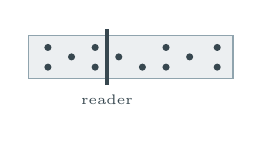
\begin{tikzpicture}
  \draw[draw=nLine, fill=nFill] (0,0) rectangle (2.6,0.55);
  \foreach \x/\y in {0.25/0.15,0.25/0.4,0.55/0.28,0.85/0.15,0.85/0.4,1.15/0.28,1.45/0.15,1.75/0.4,1.75/0.15,2.05/0.28,2.4/0.15,2.4/0.4}
    {\fill[nInk] (\x,\y) circle (0.045);}
  \draw[nInk, very thick] (1.0,-0.08) -- (1.0,0.63);
  \node[font=\tiny, text=nInk, anchor=north] at (1.0,-0.08) {reader};
\end{tikzpicture}}

\newcommand{\diagMemStackSmall}{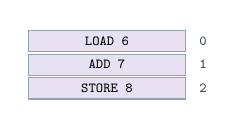
\begin{tikzpicture}
  \node[smallcell, fill=sViolet!18, minimum width=2.0cm] at (0,0.3) {LOAD 6};
  \node[smallcell, fill=sViolet!18, minimum width=2.0cm] at (0,0) {ADD 7};
  \node[smallcell, fill=sViolet!18, minimum width=2.0cm] at (0,-0.3) {STORE 8};
  \node[addr, font=\ttfamily\tiny, anchor=west] at (1.05,0.3) {0};
  \node[addr, font=\ttfamily\tiny, anchor=west] at (1.05,0) {1};
  \node[addr, font=\ttfamily\tiny, anchor=west] at (1.05,-0.3) {2};
\end{tikzpicture}}

\newcommand{\diagTwoMem}{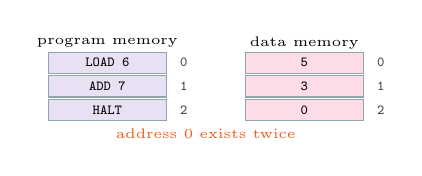
\begin{tikzpicture}
  \node[font=\tiny] at (0,0.55) {program memory};
  \node[font=\tiny] at (2.5,0.55) {data memory};
  \node[smallcell, fill=sViolet!18, minimum width=1.5cm] at (0,0.3) {LOAD 6};
  \node[smallcell, fill=sViolet!18, minimum width=1.5cm] at (0,0) {ADD 7};
  \node[smallcell, fill=sViolet!18, minimum width=1.5cm] at (0,-0.3) {HALT};
  \node[smallcell, fill=sPink!18, minimum width=1.5cm] at (2.5,0.3) {5};
  \node[smallcell, fill=sPink!18, minimum width=1.5cm] at (2.5,0) {3};
  \node[smallcell, fill=sPink!18, minimum width=1.5cm] at (2.5,-0.3) {0};
  \foreach \i in {0,1,2} {
    \node[addr, font=\ttfamily\tiny, anchor=west] at (0.8,{0.3-0.3*\i}) {\i};
    \node[addr, font=\ttfamily\tiny, anchor=west] at (3.3,{0.3-0.3*\i}) {\i};
  }
  \node[font=\tiny, text=AccentOrange] at (1.25,-0.6) {address 0 exists twice};
\end{tikzpicture}}

\newcommand{\diagOneMem}{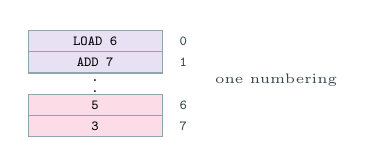
\begin{tikzpicture}
  \node[smallcell, fill=sViolet!18, minimum width=1.7cm] (o0) at (0,0.5) {LOAD 6};
  \node[smallcell, fill=sViolet!18, minimum width=1.7cm] at (0,0.23) {ADD 7};
  \node[smallcell, draw=none, minimum width=1.7cm] at (0,-0.04) {$\vdots$};
  \node[smallcell, fill=sPink!18, minimum width=1.7cm] at (0,-0.31) {5};
  \node[smallcell, fill=sPink!18, minimum width=1.7cm] at (0,-0.58) {3};
  \node[addr, font=\ttfamily\tiny, anchor=west] at (0.95,0.5) {0};
  \node[addr, font=\ttfamily\tiny, anchor=west] at (0.95,0.23) {1};
  \node[addr, font=\ttfamily\tiny, anchor=west] at (0.95,-0.31) {6};
  \node[addr, font=\ttfamily\tiny, anchor=west] at (0.95,-0.58) {7};
  \node[font=\tiny, text=nInk, anchor=west] at (1.4,0) {one numbering};
\end{tikzpicture}}

\newcommand{\diagDecimal}{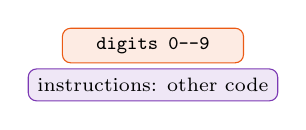
\begin{tikzpicture}
  \node[draw=AccentOrange, fill=AccentOrange!12, rounded corners=3pt, font=\ttfamily\scriptsize, minimum height=0.4cm,
    minimum width=2.3cm] at (0,0.28) {digits 0--9};
  \node[draw=ProgramPurple, fill=ProgramPurple!12, rounded corners=3pt, font=\scriptsize, minimum height=0.4cm,
    minimum width=2.3cm] at (0,-0.22) {instructions: other code};
\end{tikzpicture}}

\newcommand{\diagBinary}{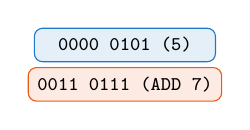
\begin{tikzpicture}
  \node[draw=StorageBlue, fill=StorageBlue!12, rounded corners=3pt, font=\ttfamily\scriptsize, minimum height=0.4cm,
    minimum width=2.3cm] at (0,0.28) {0000 0101 (5)};
  \node[draw=AccentOrange, fill=AccentOrange!12, rounded corners=3pt, font=\ttfamily\scriptsize, minimum height=0.4cm,
    minimum width=2.3cm] at (0,-0.22) {0011 0111 (ADD 7)};
\end{tikzpicture}}

\newcommand{\diagParallel}{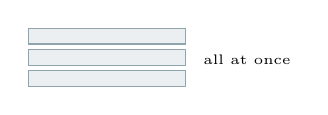
\begin{tikzpicture}
  \foreach \k in {0,1,2} {\draw[fill=nFill, draw=nLine] (0,{0.6-0.27*\k}) rectangle (2.0,{0.4-0.27*\k});}
  \node[font=\tiny, anchor=west] at (2.1,0.2) {all at once};
\end{tikzpicture}}

\newcommand{\diagDataflow}{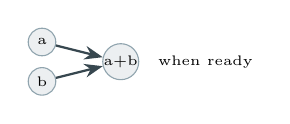
\begin{tikzpicture}[>=Stealth]
  \node[circle, draw=nLine, fill=nFill, minimum size=0.35cm, inner sep=0pt, font=\tiny] (a) at (0,0.3) {a};
  \node[circle, draw=nLine, fill=nFill, minimum size=0.35cm, inner sep=0pt, font=\tiny] (b) at (0,-0.2) {b};
  \node[circle, draw=nLine, fill=nFill, minimum size=0.4cm, inner sep=0pt, font=\tiny] (c) at (1.0,0.05) {a+b};
  \draw[->, thick, nInk] (a) -- (c); \draw[->, thick, nInk] (b) -- (c);
  \node[font=\tiny, anchor=west] at (1.35,0.05) {when ready};
\end{tikzpicture}}

\newcommand{\diagSequential}{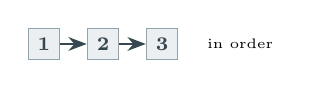
\begin{tikzpicture}[>=Stealth]
  \foreach \k in {1,2,3} {\node[draw=nLine, fill=nFill, text=nInk, minimum size=0.4cm, inner sep=0pt, font=\scriptsize\bfseries]
    (s\k) at ({0.75*\k-0.75},0.05) {\k};}
  \draw[->, thick, nInk] (s1) -- (s2); \draw[->, thick, nInk] (s2) -- (s3);
  \node[font=\tiny, anchor=west] at (1.95,0.05) {in order};
\end{tikzpicture}}

\newcommand{\diagMonolith}{
\begin{tikzpicture}
  \node[draw=nLine, very thick, rounded corners=4pt, fill=nFill, text=nInk, minimum width=2.6cm, minimum height=0.85cm,
    font=\scriptsize, align=center] {one block:\\[-1pt]everything mixed together};
\end{tikzpicture}}

\newcommand{\diagUnits}{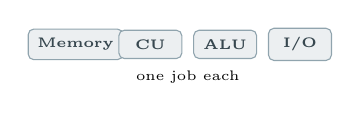
\begin{tikzpicture}
  \node[draw=nLine, fill=nFill, text=nInk, rounded corners=2pt, font=\tiny\bfseries, minimum width=0.8cm, minimum height=0.36cm] at (0,0.22) {Memory};
  \node[draw=nLine, fill=nFill, text=nInk, rounded corners=2pt, font=\tiny\bfseries, minimum width=0.8cm, minimum height=0.36cm] at (0.95,0.22) {CU};
  \node[draw=nLine, fill=nFill, text=nInk, rounded corners=2pt, font=\tiny\bfseries, minimum width=0.8cm, minimum height=0.36cm] at (1.9,0.22) {ALU};
  \node[draw=nLine, fill=nFill, text=nInk, rounded corners=2pt, font=\tiny\bfseries, minimum width=0.8cm, minimum height=0.36cm] at (2.85,0.22) {I/O};
  \node[font=\tiny] at (1.425,-0.2) {one job each};
\end{tikzpicture}}

% ---------- helpers for the CPU section ----------
\tikzset{
  reg/.style={draw=nLine, very thick, fill=white, text=nInk, rounded corners=2pt,
    minimum width=1.95cm, minimum height=0.55cm, inner sep=2pt, font=\ttfamily\scriptsize, align=center},
  cpuunit/.style={very thick, rounded corners=3pt, minimum width=1.2cm, minimum height=0.6cm,
    inner sep=2pt, font=\scriptsize\bfseries, align=center},
  hot/.style={aexec, label={[text=aExec, inner sep=1pt, font=\tiny]right:$\blacktriangleleft$}},
  hotdata/.style={aread},
  hotwrite/.style={awrite},
  hotalu/.style={aexec},
  fetcharrow/.style={-{Stealth}, very thick, DeepBlue, rounded corners=3pt},
  dataarrow/.style={-{Stealth}, very thick, DeepBlue, rounded corners=3pt},
  steplabel/.style={font=\tiny\bfseries, fill=white, inner sep=1pt},
}
% memory with the running example
% #1 highlighted instruction (0-3, -1 = none)  #2 text of cell 8  #3 highlighted data cell (6-8, 0 = none)
\newcommand{\mempanel}[3]{%
  \node[font=\scriptsize\bfseries, text=nInk] at (0,1.8) {Memory};
  \foreach \i/\t in {0/{0001 0110\ \ LOAD 6},1/{0011 0111\ \ ADD 7},2/{0010 1000\ \ STORE 8},3/{0111 0000\ \ HALT}} {
    \ifnum\i=#1
      \node[instrcell, minimum width=2.9cm, hot] (m\i) at (0,{1.35-0.45*\i}) {\t};
    \else
      \node[instrcell, minimum width=2.9cm] (m\i) at (0,{1.35-0.45*\i}) {\t};
    \fi
    \node[addr, anchor=east] at (-1.5,{1.35-0.45*\i}) {\i};
  }
  \node[memcell, draw=none, minimum width=2.9cm] at (0,-0.45) {$\vdots$};
  \foreach \i/\t/\y in {6/{0000 0101\ \ (5)}/-0.9,7/{0000 0011\ \ (3)}/-1.35,8/{#2}/-1.8} {
    \ifnum\i=#3
      \ifnum\i=8 \node[datacell, minimum width=2.9cm, hotwrite] (m\i) at (0,\y) {\t};\else \node[datacell, minimum width=2.9cm, hotdata] (m\i) at (0,\y) {\t};\fi
    \else
      \node[datacell, minimum width=2.9cm] (m\i) at (0,\y) {\t};
    \fi
    \node[addr, anchor=east] at (-1.5,\y) {\i};
  }
}
% the CPU, built up step by step
% #1 level: 0 empty, 1 +PC, 2 +IR, 3 +AC, 4 +ALU, 5 +CU   #2 PC   #3 IR   #4 AC   #5 extra ALU style
\newcommand{\cpupanel}[5]{%
  \node[draw=nLine, very thick, rounded corners=6pt, fill=nFill!50, minimum width=4.65cm,
    minimum height=3.85cm, anchor=west] (cpu) at (2.45,-0.2) {};
  \node[font=\scriptsize\bfseries, text=nInk, anchor=north west] at ([shift={(0.1,-0.06)}]cpu.north west) {CPU};
  \ifnum#1>0 \node[reg] (pc) at (3.65,0.95) {\textbf{PC}\ \ #2}; \fi
  \ifnum#1>1 \node[reg] (ir) at (3.65,0.0) {\textbf{IR}\\[-1pt]#3}; \fi
  \ifnum#1>2 \node[reg] (ac) at (3.65,-1.05) {\textbf{AC}\ \ #4}; \fi
  \ifnum#1>3 \node[cpuunit, draw=mygreen, fill=mygreen!18, #5] (alu) at (6.3,-1.05)
    {\textcolor{mygreen!60!black}{\faCalculator}\\[-1pt]ALU}; \fi
  \ifnum#1>4 \node[cpuunit, draw=AccentOrange, fill=AccentOrange!18] (cu) at (6.3,0.5)
    {\textcolor{AccentOrange}{\faCogs}\\[-1pt]CU}; \fi
}
% explanation slide: #1 title, #2 tikz body (memory + CPU), #3 right-hand column
\newcommand{\explainframe}[3]{%
\begin{frame}{#1}
  \begin{columns}[c,onlytextwidth]
    \column{0.58\textwidth}
      \centering
      \begin{tikzpicture}[>=Stealth, scale=0.92, every node/.append style={transform shape}]
        #2
      \end{tikzpicture}
    \column{0.4\textwidth}
      #3
  \end{columns}
\end{frame}}
% boxes for the right-hand column
\newcommand{\defbox}[1]{%
  \begin{beamercolorbox}[rounded=true,sep=0.1cm,wd=\linewidth]{block body example}
    \footnotesize #1
  \end{beamercolorbox}\vspace{0.06cm}}
\newcommand{\stepbox}[2]{%
  \begin{beamercolorbox}[rounded=true,sep=0.09cm,wd=\linewidth]{block body}
    \footnotesize\textbf{#1}\\ #2
  \end{beamercolorbox}\vspace{0.06cm}}
\newcommand{\phasename}[1]{%
  {\centering\footnotesize Name of this phase:\ \colorbox{DeepBlue}{\textcolor{white}{\textbf{#1}}}\par}}
% small tag above the CPU box: which instruction is being executed
\newcommand{\executing}[1]{%
  \node[font=\scriptsize\bfseries, text=AccentOrange, anchor=south east] at ([yshift=1pt]cpu.north east)
    {Executing: \texttt{#1}};}
\newcommand{\statebox}[1]{%
  {\centering\scriptsize\textcolor{DeepBlue}{\textbf{State:}}\ #1\par}}

\lstset{
  language=Python,
  basicstyle=\color{VSText}\ttfamily\footnotesize,
  keywordstyle=\color{VSPurple}\bfseries,
  stringstyle=\color{VSString},
  commentstyle=\color{VSComment}\itshape,
  numbers=left,
  numberstyle=\tiny\color{gray},
  stepnumber=1,
  breaklines=true,
  showstringspaces=false,
  xleftmargin=15pt,
  xrightmargin=5pt,
  frame=none
}

% MARIE assembly: line numbers start at 0, so a line number equals the memory address
\lstdefinelanguage{MARIE}{
  morekeywords={Load,Store,Add,Subt,Input,Output,Halt,Jump,Skipcond,DEC,HEX,ADR,LoadI,StoreI,AddI,JumpI,JnS,Clear,LoadImmi},
  sensitive=false,
  comment=[l]{/},
}
\lstdefinestyle{marie}{language=MARIE, firstnumber=0, basicstyle=\color{VSText}\ttfamily\scriptsize,
  keywordstyle=\color{VSBlue}\bfseries, commentstyle=\color{VSComment}\itshape,
  columns=fixed, basewidth=0.52em, keepspaces=true, breaklines=false, xleftmargin=12pt}

\BeforeBeginEnvironment{lstlisting}{%
  \begin{beamercolorbox}[rounded=true,sep=2mm,wd=\linewidth]{vscodelisting}%
  
\begin{tikzpicture}
    \fill[nLine] (0,0) circle (3pt);
    \fill[nLine] (0.35,0) circle (3pt);
    \fill[nLine] (0.70,0) circle (3pt);
  \end{tikzpicture}%
  \vspace{-0.2cm}%
}
\AfterEndEnvironment{lstlisting}{\end{beamercolorbox}}

% =====================================================================
%  Day 2 helpers
% =====================================================================

% ---------- MARIE datapath, drawn like the Data Path view of MARIE.js ----------
% \busdiagram[values]{source}{destination}{extra TikZ}
%   source (Read, blue) and destination (Write, red): ir, out, in, ac, mbr, pc, mar, mem, none
%   values: ir=, out=, in=, ac=, mbr=, pc=, mar=, mem= (contents of M[MAR]), step= (0-7, -1 = none)
\definecolor{ReadBlue}{HTML}{1E88E5}
\definecolor{WriteRed}{HTML}{E53935}
\definecolor{BusGreen}{HTML}{B0BEC5}% the bus: neutral
\tikzset{
  dpreg/.style={draw=nLine, thick, fill=white, text=nInk, minimum width=1.1cm, minimum height=0.46cm,
    inner sep=1pt, font=\ttfamily\scriptsize},
  dpname/.style={font=\tiny, text=nInk, above=0pt, inner sep=1pt},
  dpwire/.style={thin, nLight},
  dpmem/.style={draw=nLine, very thick, fill=nFill, rounded corners=3pt,
    minimum width=1.3cm, minimum height=0.95cm, font=\scriptsize\bfseries, align=center},
  srcreg/.style={draw=ReadBlue, line width=1.6pt},
  dstreg/.style={draw=WriteRed, line width=1.6pt},
}
\pgfkeys{/dp/.is family, /dp,
  ir/.initial={0000}, out/.initial={0000}, in/.initial={0000}, ac/.initial={0000},
  mbr/.initial={0000}, pc/.initial={000}, mar/.initial={000}, mem/.initial={0000},
  step/.initial={-1}}
\newcommand{\dpv}[1]{\pgfkeysvalueof{/dp/#1}}
\newcommand{\busdiagram}[4][]{%
  \begingroup
  \pgfkeys{/dp, ir=0000, out=0000, in=0000, ac=0000, mbr=0000, pc=000, mar=000, mem=0000, step=-1, #1}%
  \begin{tikzpicture}[>=Stealth]
    \tikzset{bd-mem/.style={}, bd-mar/.style={}, bd-pc/.style={}, bd-mbr/.style={},
      bd-ac/.style={}, bd-ir/.style={}, bd-in/.style={}, bd-out/.style={}, bd-none/.style={}}
    \tikzset{bd-#2/.style={srcreg}}
    \tikzset{bd-#3/.style={dstreg}}
    % ----- control unit -----
    \node[draw=DeepBlue!80, thick, fill=white, minimum width=1.3cm, minimum height=2.95cm,
      anchor=north west] (cu) at (-2.4,2.0) {};
    \node[font=\tiny, text=DeepBlue, anchor=north west, below=1pt] at (cu.south west) {Control unit};
    \node[font=\tiny, text=DeepBlue!80, anchor=east] at (-1.15,1.75) {Read};
    \node[font=\tiny, text=DeepBlue!80, anchor=east] at (-1.15,-0.6) {Write};
    \node[font=\tiny, text=DeepBlue!80, anchor=east] at (-1.15,0.05) {AC<0};
    \node[font=\tiny, text=DeepBlue!80, anchor=east] at (-1.15,-0.15) {AC=0};
    \node[font=\tiny, text=DeepBlue!80] at (-2.0,1.3) {Step};
    \foreach \k in {0,...,7} {
      \pgfmathtruncatemacro{\cur}{\dpv{step}}
      \ifnum\k=\cur
        \fill[AccentOrange] (-2.0,{1.1-0.15*\k}) circle (0.065);
      \else
        \fill[DeepBlue!30] (-2.0,{1.1-0.15*\k}) circle (0.035);
      \fi
    }
    % ----- memory -----
    \node[draw=DeepBlue!80, thick, fill=white, minimum width=1.5cm, minimum height=2.95cm,
      anchor=north west, bd-mem] (mem) at (10.4,2.0) {};
    \node[font=\tiny, text=DeepBlue, anchor=north west, below=1pt] at (mem.south west) {Main memory};
    \node[font=\ttfamily\tiny, text=DeepBlue!80] at (11.15,0.75) {M[MAR]};
    \node[font=\ttfamily\scriptsize] at (11.15,0.5) {\dpv{mem}};
    % ----- faint control wires (one Read and one Write wire per device) -----
    \draw[dpwire] (-1.1,1.75) -- (10.4,1.75);
    \draw[dpwire] (-1.1,-0.6) -- (10.4,-0.6);
    \foreach \x in {0.6,2.0,3.4,4.8,6.2,7.6,9.0} {
      \draw[dpwire] (\x-0.25,1.75) -- (\x-0.25,1.18);
      \draw[dpwire] (\x+0.3,-0.6) -- (\x+0.3,0.72);
    }
    % ----- bus (drawn first, registers on top) -----
    \foreach \x in {0.6,2.0,3.4,4.8,6.2,7.6,9.0}
      \draw[line width=2.6pt, BusGreen] (\x,0.72) -- (\x,-0.35);
    \draw[line width=2.6pt, BusGreen] (0.6-0.045,-0.35) -- (10.4,-0.35);
    % ----- ALU between AC and MBR, with its links and the flag wires to the CU -----
    \draw[thin, DeepBlue!40] (4.45,0.05) -- (-1.1,0.05);
    \draw[thin, DeepBlue!40] (4.45,-0.15) -- (-1.1,-0.15);
    \draw[thick, DeepBlue!70, fill=white] (5.0,0.47) -- (5.42,0.47) -- (5.5,0.37) -- (5.58,0.47) -- (6.0,0.47)
      -- (5.72,0.05) -- (5.28,0.05) -- cycle;
    \node[font=\tiny, text=DeepBlue!80] at (5.5,0.22) {ALU};
    \draw[thick, DeepBlue!60] (5.2,0.72) -- (5.2,0.47);
    \draw[thick, DeepBlue!60] (5.8,0.72) -- (5.8,0.47);
    \draw[thick, DeepBlue!60] (5.5,0.05) -- (5.5,-0.1) -- (4.45,-0.1) |- (4.45,0.72);
    % ----- registers -----
    \foreach \n/\x/\lab in {ir/0.6/IR, out/2.0/OUT, in/3.4/IN, ac/4.8/AC, mbr/6.2/MBR, pc/7.6/PC, mar/9.0/MAR} {
      \node[dpreg, bd-\n] (\n) at (\x,0.95) {\dpv{\n}};
      \node[dpname] at (\n.north) {\lab};
      \coordinate (\n-port) at (\n.south);
      \coordinate (\n-bus) at (\x,-0.35);
    }
    \coordinate (mem-port) at (10.4,-0.35);
    \coordinate (mem-bus) at (10.4,-0.35);
    % IR is decoded by the CU; MAR selects the memory cell
    \draw[thick, BusGreen, -{Stealth}] (ir.west) -- (-1.1,0.95);
    \draw[thick, BusGreen, -{Stealth}] (mar.east) -- (10.4,0.95);
    % ----- active Read and Write signals -----
    \ifstrequal{#2}{none}{}{%
      \ifstrequal{#2}{mem}
        {\draw[line width=1.3pt, ReadBlue, -{Stealth}] (-1.1,1.75) -- (10.4,1.75);}
        {\draw[line width=1.3pt, ReadBlue, -{Stealth}] (-1.1,1.75) -| ($(#2.north)+(-0.25,0)$);}}
    \ifstrequal{#3}{none}{}{%
      \ifstrequal{#3}{mem}
        {\draw[line width=1.3pt, WriteRed, -{Stealth}] (-1.1,-0.6) -- (10.4,-0.6);}
        {\draw[line width=1.3pt, WriteRed, -{Stealth}] (-1.1,-0.6) -| ($(#3.south)+(0.3,0)$);}}
    % ----- the value travelling along the bus -----
    \ifstrequal{#2}{none}{}{\ifstrequal{#3}{none}{}{%
      \draw[line width=3pt, nInk] (#2-port) -- (#2-bus) -- (#3-bus) -- (#3-port);
      \draw[line width=1.5pt, white, dash pattern=on 1.5pt off 1.5pt] (#2-port) -- (#2-bus) -- (#3-bus) -- (#3-port);}}
    #4
  \end{tikzpicture}%
  \endgroup}

% legend for the colours of the data path
\newcommand{\dplegend}{%
  {\tiny\textcolor{ReadBlue}{\rule{0.25cm}{0.2cm}}\ \textbf{Read}: puts its value on the bus
  \qquad\textcolor{WriteRed}{\rule{0.25cm}{0.2cm}}\ \textbf{Write}: stores the value from the bus
  \qquad\tikz[baseline=-0.6ex]{\draw[line width=3pt, BusGreen] (0,0) -- (0.5,0);\draw[line width=1.5pt, white, dash pattern=on 1.5pt off 1.5pt] (0,0) -- (0.5,0);}\ the value travelling on the bus}}

% one step of an instruction: data path on top, explanation below
% #1 title, #2 source, #3 destination, #4 values (keys), #5 explanation
\newcommand{\stepframe}[5]{%
\begin{frame}{#1}
  \begin{center}
    \resizebox{0.8\textwidth}{!}{\busdiagram[#4]{#2}{#3}{}}\\[0.02cm]
    \dplegend
  \end{center}
  \vspace{-0.1cm}
  \begin{center}
    \begin{minipage}{0.8\textwidth}
      #5
    \end{minipage}
  \end{center}
\end{frame}}

% ---------- timeline of clock steps ----------
% #1 fetch steps, #2 execute steps, #3 label on the right
\newcommand{\steptimeline}[3]{%
  \begin{tikzpicture}
    \foreach \i in {1,...,#1}
      \node[draw=white, fill=sAmber, text=black, font=\tiny\bfseries, minimum width=0.62cm,
        minimum height=0.45cm, inner sep=0pt] at ({0.62*(\i-1)},0) {T\the\numexpr\i-1\relax};
    \foreach \i in {1,...,#2}
      \node[draw=white, fill=sTeal, text=white, font=\tiny\bfseries, minimum width=0.62cm,
        minimum height=0.45cm, inner sep=0pt] at ({0.62*(#1+\i-1)},0) {T\the\numexpr#1+\i-1\relax};
    \node[anchor=west, font=\scriptsize] at ({0.62*(#1+#2)-0.25},0) {#3};
  \end{tikzpicture}}

% legend for the timeline colours
\newcommand{\timelinelegend}{%
  {\tiny\textcolor{StorageBlue!75}{\rule{0.25cm}{0.2cm}}\ fetch
  \qquad\textcolor{AccentOrange}{\rule{0.25cm}{0.2cm}}\ execute}}

% ---------- small pieces for the addressing-mode slides ----------
\tikzset{
  mcell/.style={draw=DeepBlue!60, minimum width=1.5cm, minimum height=0.42cm, inner sep=1pt,
    font=\ttfamily\scriptsize, align=center, fill=StorageBlue!15},
  mcellhot/.style={mcell, fill=StorageBlue!45, draw=StorageBlue, very thick},
  mcellptr/.style={mcell, fill=ProgramPurple!18, draw=ProgramPurple, very thick},
  instrbox/.style={draw=AccentOrange, very thick, fill=AccentOrange!15, rounded corners=2pt,
    minimum height=0.5cm, inner sep=3pt, font=\ttfamily\scriptsize},
  ptrarrow/.style={-{Stealth}, very thick, DeepBlue},
  valarrow/.style={-{Stealth}, very thick, DeepBlue},
}

% task header box (same look as on Day 1)
% #1 form and time, #2 short instruction
\newcommand{\taskhead}[2]{%
  \begin{beamercolorbox}[rounded=true,sep=0.12cm,wd=\linewidth]{block body example}
    \small\textbf{#1}\\[0.04cm]
    \footnotesize #2
  \end{beamercolorbox}\vspace{0.1cm}}

% highlighted key message at the bottom of a slide
\newcommand{\keymsg}[1]{%
  \begin{beamercolorbox}[rounded=true,sep=0.1cm,wd=\textwidth]{block body example}
    \centering\footnotesize #1
  \end{beamercolorbox}}

% register transfer written in text: \mo{MAR}{PC} gives MAR <- PC
\newcommand{\mo}[2]{\texttt{#1\,$\leftarrow$\,#2}}

% plain listings (x86, RISC-V) without Python highlighting
\lstdefinelanguage{plain}{}
\lstdefinestyle{asm}{language=plain, basicstyle=\color{VSText}\ttfamily\scriptsize, numbers=none,
  columns=fixed, basewidth=0.52em, keepspaces=true, xleftmargin=6pt}

% =====================================================================
%  Day 3 helpers
% =====================================================================

\usetikzlibrary{patterns}
\usepackage{multirow}
% ---------- RISC-V listings ----------
\lstdefinestyle{rv}{language=RISCV, basicstyle=\color{VSText}\ttfamily\scriptsize, numbers=none,
  keywordstyle=\color{VSBlue}\bfseries, keywordstyle={[2]\color{VSPurple}\bfseries},
  commentstyle=\color{VSComment}\itshape,
  columns=fixed, basewidth=0.52em, keepspaces=true, breaklines=false, xleftmargin=6pt}
\lstdefinestyle{rvnum}{style=rv, numbers=left, firstnumber=1, xleftmargin=14pt}

% ---------- colours of the five pipeline stages (the same all day) ----------
\colorlet{cIF}{sAmber}
\colorlet{cID}{sBrown}
\colorlet{cEX}{sTeal}
\colorlet{cMEM}{sIndigo}
\colorlet{cWB}{sPink}
% text on a stage colour (amber needs black)
\colorlet{txIF}{black}\colorlet{txID}{white}\colorlet{txEX}{white}\colorlet{txMEM}{white}\colorlet{txWB}{white}
\colorlet{txcIF}{black}\colorlet{txcID}{white}\colorlet{txcEX}{white}\colorlet{txcMEM}{white}\colorlet{txcWB}{white}

% ---------- pipeline diagrams ----------
% cell size (cm)
\def\pw{0.74}
\def\ph{0.46}
\tikzset{
  pcell/.style={minimum width=\pw cm, minimum height=\ph cm, inner sep=0pt, draw=white,
    font=\scriptsize\bfseries, text=white},
  pst-IF/.style={pcell, fill=cIF, text=black},
  pst-ID/.style={pcell, fill=cID},
  pst-EX/.style={pcell, fill=cEX},
  pst-MEM/.style={pcell, fill=cMEM},
  pst-WB/.style={pcell, fill=cWB},
  pst-B/.style={pcell, fill=nIdle, text=nInk, font=\tiny},
  pst-X/.style={pcell, fill=nFill, text=nInk, draw=nLine},
  pst-N/.style={pcell, fill=none, draw=none},
  pst-E/.style={pcell, fill=nFill!60},
  plab/.style={anchor=east, font=\ttfamily\footnotesize, inner sep=1pt},
}
% one row of a pipeline diagram
% #1 row (0 = top), #2 first cycle (1-based), #3 comma list of IF, ID, EX, MEM, WB, B (bubble), X (flushed), N (empty)
\newcommand{\prow}[3]{%
  \foreach \s [count=\k from 0] in {#3} {%
    \node[pst-\s] at ({(#2+\k-1)*\pw}, {-(#1)*\ph}) {%
      \expandafter\ifstrequal\expandafter{\s}{B}{bubble}{%
      \expandafter\ifstrequal\expandafter{\s}{X}{$\times$}{%
      \expandafter\ifstrequal\expandafter{\s}{N}{}{\expandafter\ifstrequal\expandafter{\s}{E}{}{\s}}}}};
  }}
% label of a row
\newcommand{\plabel}[2]{\node[plab] at ({-0.5*\pw-0.05}, {-(#1)*\ph}) {#2};}
% cycle numbers above the diagram: #1 number of cycles
\newcommand{\pcycles}[1]{%
  \foreach \c in {1,...,#1}
    \node[font=\scriptsize, text=DeepBlue!70] at ({(\c-1)*\pw}, {0.8*\ph}) {\c};
  \node[font=\scriptsize, text=DeepBlue!70, anchor=east] at ({-0.5*\pw-0.05}, {0.8*\ph}) {cycle};}
% highlight one column: #1 cycle, #2 number of rows, #3 colour
\newcommand{\pcolumn}[3]{%
  \draw[#3, very thick, rounded corners=2pt]
    ({(#1-1.5)*\pw}, {0.5*\ph}) rectangle ({(#1-0.5)*\pw}, {-(#2-0.5)*\ph});}

% legend of stage colours
\newcommand{\stagelegend}{%
  {\tiny
  \textcolor{cIF}{\rule{0.25cm}{0.2cm}}\,IF fetch\quad
  \textcolor{cID}{\rule{0.25cm}{0.2cm}}\,ID decode\quad
  \textcolor{cEX}{\rule{0.25cm}{0.2cm}}\,EX execute\quad
  \textcolor{cMEM}{\rule{0.25cm}{0.2cm}}\,MEM memory\quad
  \textcolor{cWB}{\rule{0.25cm}{0.2cm}}\,WB write back}}

% ---------- stage boxes ----------
\tikzset{
  stagebox/.style={very thick, rounded corners=4pt, minimum width=1.9cm, minimum height=0.8cm,
    align=center, font=\small\bfseries, drop shadow},
  gbar/.style={minimum height=0.36cm, inner sep=0pt, draw=white, font=\tiny\bfseries, text=white},
  gempty/.style={minimum height=0.36cm, inner sep=0pt, draw=gray!50, dashed, font=\tiny, text=gray!60},
  unit/.style={draw=nLine, very thick, fill=white, text=nInk, rounded corners=3pt, align=center,
    font=\scriptsize\bfseries, inner sep=2pt},
}

% ---------- a simple RISC-V datapath ----------
% #1 extra TikZ drawn on top (nodes: pc, imem, rf, alu, dmem, mux, cu, add4)
\newcommand{\rvdatapath}[1]{%
  \begin{tikzpicture}[>=Stealth, font=\scriptsize]
    % stage labels
    \foreach \x/\n/\c in {0.9/IF/cIF, 4.2/ID/cID, 6.6/EX/cEX, 9.0/MEM/cMEM, 10.9/WB/cWB}
      \node[fill=\c, text=tx\c, rounded corners=2pt, font=\tiny\bfseries, minimum width=0.9cm] at (\x,2.35) {\n};
    % units
    \node[unit, minimum width=0.6cm, minimum height=1.0cm] (pc) at (0,0) {PC};
    \node[unit, minimum width=1.5cm, minimum height=1.6cm] (imem) at (1.8,0) {Instruction\\memory};
    \node[unit, minimum width=1.5cm, minimum height=1.8cm] (rf) at (4.2,0) {Register\\file};
    \draw[nInk, very thick, fill=white] (6.2,0.9) -- (7.0,0.45) -- (7.0,-0.45) -- (6.2,-0.9) -- (6.2,-0.25)
      -- (6.4,0) -- (6.2,0.25) -- cycle;
    \node[font=\scriptsize\bfseries] (alu) at (6.68,0) {ALU};
    \coordinate (aluin1) at (6.2,0.55); \coordinate (aluin2) at (6.2,-0.55); \coordinate (aluout) at (7.0,0);
    \node[unit, minimum width=1.5cm, minimum height=1.6cm] (dmem) at (9.0,0) {Data\\memory};
    \node[unit, minimum width=0.45cm, minimum height=1.2cm, rounded corners=6pt, font=\tiny] (mux) at (10.9,0) {M\\U\\X};
    \node[unit, minimum width=1.3cm, minimum height=0.5cm, draw=nLine, text=nLine] (add4) at (0.9,1.55) {$+4$};
    \node[unit, minimum width=2.2cm, minimum height=0.5cm, draw=gray, text=gray] (cu) at (4.2,-1.85) {Control unit};
    % wires
    \draw[->, thick] (pc) -- (imem);
    \draw[->, thick] (imem) -- node[above, font=\tiny] {instruction} (rf);
    \draw[->, thick] ([yshift=0.55cm]rf.east) -- (aluin1);
    \draw[->, thick] ([yshift=-0.55cm]rf.east) -- (aluin2);
    \draw[->, thick] (aluout) -- node[above, font=\tiny] {address} ([yshift=0cm]dmem.west);
    \draw[->, thick] ([yshift=-0.55cm]dmem.east) -- ([yshift=-0.4cm]mux.west);
    \draw[->, thick] (7.3,0) |- (7.3,-1.1) -| (10.3,-1.1) |- ([yshift=0.4cm]mux.west);
    \draw[->, thick] (mux.east) -- ++(0.3,0) |- (11.2,2.0) -| node[pos=0.25, above, font=\tiny] {write back} (4.2,0.9);
    \draw[->, thick, DeepBlue!60] (pc.north) |- (add4.west);
    \draw[->, thick, DeepBlue!60] (add4.east) -- ++(0.35,0) |- (-0.6,1.95) |- (pc.west);
    \draw[->, dashed, gray] (cu.north) -- (rf.south);
    \draw[->, dashed, gray] (cu.east) -| (dmem.south);
    \draw[->, dashed, gray] (cu.east) -| (mux.south);
    #1
  \end{tikzpicture}}

% ---------- Ripes window (schematic; replace with a real screenshot if you like) ----------
\newcommand{\ripeswindow}{%
  \begin{tikzpicture}[font=\tiny]
    \draw[nInk, very thick, fill=white, rounded corners=4pt] (0,0) rectangle (9,5.4);
    \fill[nLight, rounded corners=4pt] (0,5.0) rectangle (9,5.4);
    \fill[MacRed] (0.25,5.2) circle (2.5pt); \fill[MacYellow] (0.5,5.2) circle (2.5pt); \fill[MacGreen] (0.75,5.2) circle (2.5pt);
    \node[font=\tiny\bfseries, text=nInk] at (4.5,5.2) {Ripes};
    % toolbar
    \fill[LightGray] (0,4.55) rectangle (9,5.0);
    \foreach \x/\i in {1.0/\faMicrochip, 1.6/\faStepForward, 2.2/\faPlay, 2.8/\faFastForward, 3.4/\faUndo}
      \node[text=nInk] at (\x,4.77) {\i};
    % side bar
    \fill[nLine] (0,0) rectangle (0.5,4.55);
    \foreach \y/\i in {4.1/\faEdit, 3.5/\faMicrochip, 2.9/\faMemory, 2.3/\faTerminal}
      \node[text=white] at (0.25,\y) {\i};
    % editor
    \draw[gray!60, fill=VSDarkBg] (0.65,0.15) rectangle (3.2,4.4);
    \foreach \y/\t in {4.1/lw x5{,} X, 3.8/lw x6{,} Y, 3.5/add x7{,} x5{,} x6, 3.2/addi x7{,} x7{,} -2, 2.9/sw x7{,} Z{,} x28}
      \node[anchor=west, text=VSText, font=\ttfamily\tiny] at (0.75,\y) {\t};
    % processor view
    \draw[gray!60, fill=nFill] (3.35,1.4) rectangle (7.3,4.4);
    \foreach \x/\c in {3.8/cIF, 4.5/cID, 5.3/cEX, 6.1/cMEM, 6.8/cWB}
      \draw[\c, very thick, fill=\c!15] (\x-0.25,2.3) rectangle (\x+0.25,3.6);
    \draw[->, thick, DeepBlue!60] (3.55,2.95) -- (7.05,2.95);
    \node[font=\tiny, text=nInk] at (5.3,1.85) {datapath};
    % statistics
    \draw[gray!60, fill=white] (3.35,0.15) rectangle (7.3,1.25);
    \node[anchor=west, font=\tiny] at (3.45,0.95) {Cycles: 13};
    \node[anchor=west, font=\tiny] at (3.45,0.7) {Instrs. retired: 8};
    \node[anchor=west, font=\tiny] at (3.45,0.45) {CPI: 1.63 \quad IPC: 0.62};
    % registers
    \draw[gray!60, fill=white] (7.45,0.15) rectangle (8.85,4.4);
    \foreach \k [count=\j from 0] in {x5,x6,x7,x8,x9,x10}
      \node[anchor=west, font=\ttfamily\tiny] at (7.5,{4.1-0.3*\j}) {\k};
    \node[font=\tiny, text=nInk] at (8.15,2.1) {registers};
    % badges
    \node[circle, fill=AccentOrange, text=white, font=\bfseries\scriptsize, inner sep=1.5pt] at (1.9,1.2) {1};
    \node[circle, fill=AccentOrange, text=white, font=\bfseries\scriptsize, inner sep=1.5pt] at (1.35,4.77) {2};
    \node[circle, fill=AccentOrange, text=white, font=\bfseries\scriptsize, inner sep=1.5pt] at (5.3,4.1) {3};
    \node[circle, fill=AccentOrange, text=white, font=\bfseries\scriptsize, inner sep=1.5pt] at (6.95,0.7) {4};
    \node[circle, fill=AccentOrange, text=white, font=\bfseries\scriptsize, inner sep=1.5pt] at (8.15,1.4) {5};
  \end{tikzpicture}}

% small orange number used in running text
\newcommand{\badge}[1]{\tikz[baseline=(b.base)]\node[circle,fill=AccentOrange,text=white,
  inner sep=1.2pt,font=\bfseries\tiny] (b) {#1};}

% =====================================================================
%  Day 4 helpers
% =====================================================================

% ---------- colours of the memory levels (the same all day) ----------
% memory levels are hardware: neutral
\colorlet{cReg}{nInk}
\colorlet{cCache}{nInk}
\colorlet{cRAM}{nLine}
\colorlet{cDisk}{nLine}
\colorlet{cIO}{nInk}
\colorlet{HitGreen}{aExec}
\colorlet{MissRed}{aWrite}
\setbeamercolor{block body answer}{bg=aExec!8,fg=black}

% ---------- listings ----------
% RISC-V: the Day 3 keywords plus the new ones used today
\lstdefinelanguage{RISCV}{
  morekeywords={lw,sw,add,addi,sub,beq,bne,bnez,beqz,la,li,auipc,nop,ecall},
  morekeywords=[2]{.data,.text,.word,.zero},
  alsoletter={.},
  sensitive=true,
  morecomment=[l]{\#},
}
% C (for the locality examples)
\lstdefinestyle{cc}{language=C, basicstyle=\color{VSText}\ttfamily\scriptsize, numbers=none,
  keywordstyle=\color{VSBlue}\bfseries, commentstyle=\color{VSComment}\itshape,
  columns=fixed, basewidth=0.52em, keepspaces=true, breaklines=false, xleftmargin=6pt,
  moredelim=**[is][\color{MacYellow}\bfseries]{@}{@}}

% ---------- boxes for the memory levels and devices ----------
\tikzset{
  lbox/.style={very thick, rounded corners=4pt, align=center, font=\scriptsize\bfseries, inner sep=3pt},
  cpubox/.style={lbox, draw=nInk, fill=nInk, text=white},
  regbox/.style={lbox, draw=nLine, fill=nFill, text=nInk},
  cachebox/.style={lbox, draw=nLine, fill=nFill, text=nInk},
  rambox/.style={lbox, draw=nLine, fill=nFill, text=nInk},
  diskbox/.style={lbox, draw=nLine, fill=nFill, text=nInk},
  iobox/.style={lbox, draw=cIO, fill=cIO!12},
  dmabox/.style={lbox, draw=nLine, fill=nFill, text=nInk},
  osbox/.style={lbox, draw=nLine, fill=nFill, text=nInk},
  greybox/.style={lbox, draw=nLight, fill=white, text=nLine},
  arr/.style={-{Stealth}, very thick, nInk},
  okarr/.style={-{Stealth}, very thick, HitGreen},
  badarr/.style={-{Stealth}, very thick, MissRed},
  smalltxt/.style={font=\tiny, inner sep=1pt},
}

% ---------- design question box (as on the Day 1 dilemma slides) ----------
\newcommand{\designq}[1]{%
  \begin{beamercolorbox}[rounded=true,sep=0.14cm,wd=\textwidth]{block body}
    \centering\small\textbf{Design question:} #1
  \end{beamercolorbox}}
\newcommand{\whichone}{%
  {\centering\small\textcolor{DeepBlue}{\textbf{Which would you choose, and why?}}\par}}

% ---------- question card and answer card ----------
% #1 icon, #2 text
\newcommand{\qcard}[2]{%
  \begin{beamercolorbox}[rounded=true,sep=0.14cm,wd=\linewidth]{block body}
    \centering{\Large\textcolor{AccentOrange}{#1}}\\[0.12cm]
    \footnotesize #2
  \end{beamercolorbox}}
% #1 title, #2 text
\newcommand{\acard}[2]{%
  \begin{beamercolorbox}[rounded=true,sep=0.1cm,wd=\linewidth]{block body answer}
    \footnotesize\textbf{\textcolor{aExec}{\faCheck}\ #1}\\ #2
  \end{beamercolorbox}\vspace{0.06cm}}
% red "problem" box
\setbeamercolor{block body problem}{bg=AccentOrange!10,fg=black}
\newcommand{\probbox}[2]{%
  \begin{beamercolorbox}[rounded=true,sep=0.09cm,wd=\linewidth]{block body problem}
    \footnotesize\textbf{\textcolor{AccentOrange}{\faExclamationTriangle}\ #1}\\ #2
  \end{beamercolorbox}\vspace{0.06cm}}

% ---------- hits and misses ----------
\def\cw{0.62}
\def\chh{0.42}
\tikzset{
  hmcell/.style={minimum width=\cw cm, minimum height=\chh cm, inner sep=0pt, draw=white,
    font=\scriptsize\bfseries, text=white},
  hm-H/.style={hmcell, fill=white, draw=nLight, text=aExec},
  hm-M/.style={hmcell, fill=white, draw=nLight, text=aWrite},
  hm-Q/.style={hmcell, fill=nFill, draw=nLight, text=nLine},
  hm-A/.style={hmcell, draw=none, text=nInk, font=\scriptsize\ttfamily\bfseries},
}
% one row of hits and misses: #1 row (0 = top), #2 comma list of H, M, Q (Q = to fill in)
\newcommand{\hmrow}[2]{%
  \foreach \s [count=\k from 0] in {#2} {%
    \node[hm-\s] at ({\k*\cw}, {-(#1)*\chh}) {\expandafter\ifstrequal\expandafter{\s}{Q}{?}{\s}};}}
% the accessed addresses above a row: #1 row, #2 comma list
\newcommand{\hmhead}[2]{%
  \foreach \s [count=\k from 0] in {#2}
    \node[hm-A] at ({\k*\cw}, {-(#1)*\chh}) {\s};}
% label on the left of a row: #1 row, #2 text
\newcommand{\hmlabel}[2]{\node[anchor=east, font=\scriptsize, inner sep=1pt] at ({-0.5*\cw-0.08}, {-(#1)*\chh}) {#2};}
% label on the right of a row: #1 row, #2 number of cells, #3 text
\newcommand{\hmresult}[3]{\node[anchor=west, font=\scriptsize\bfseries, text=nInk, inner sep=1pt]
  at ({(#2-0.5)*\cw+0.12}, {-(#1)*\chh}) {#3};}

% ---------- a small cache (or page table) drawn as a table ----------
\tikzset{
  ctab/.style={draw=nLine, text=nInk, minimum height=0.4cm, inner sep=1pt, font=\ttfamily\scriptsize, fill=white},
  ctabh/.style={ctab, fill=nInk, text=white, font=\scriptsize\bfseries},
  ctabhit/.style={fill=HitGreen!25, draw=HitGreen, very thick},
  ctabmiss/.style={fill=MissRed!20, draw=MissRed, very thick},
}
% #1 comma list of line/valid/tag/data ; columns: Line, V, Tag, Data (top-left corner at the origin)
\newcommand{\cachetable}[1]{%
  \node[ctabh, minimum width=0.9cm] at (0,0) {Line};
  \node[ctabh, minimum width=0.7cm] at (0.8,0) {V};
  \node[ctabh, minimum width=1.0cm] at (1.65,0) {Tag};
  \node[ctabh, minimum width=1.6cm] at (2.95,0) {Data};
  \foreach \xa/\xb/\xc/\xd [count=\k from 1] in {#1} {
    \node[ctab, minimum width=0.9cm] (cl\k) at (0,{-0.4*\k}) {\xa};
    \node[ctab, minimum width=0.7cm] (cv\k) at (0.8,{-0.4*\k}) {\xb};
    \node[ctab, minimum width=1.0cm] (ct\k) at (1.65,{-0.4*\k}) {\xc};
    \node[ctab, minimum width=1.6cm] (cd\k) at (2.95,{-0.4*\k}) {\xd};
  }}

% ---------- timelines (polling, interrupts, DMA, bus use) ----------
% #1 y, #2 label on the left, #3 comma list of length/colour/text
\newcommand{\tlbar}[3]{%
  \node[anchor=east, font=\scriptsize\bfseries, text=nInk, align=right] at (-0.1,#1) {#2};
  \gdef\tlx{0}%
  \foreach \tlw/\tlc/\tlt in {#3} {%
    \edef\tlcc{\tlc}\def\tlpoll{cPoll}\def\tlidle{cIdle}\def\tlb{cTaskB}%
    \def\tltext{nInk}\def\tlwa{cTaskA}\def\tlwc{cTaskC}\def\tlwh{cTaskH}\def\tlwm{cWork}\def\tlwi{cISR}%
    \ifx\tlcc\tlwa\def\tltext{white}\fi\ifx\tlcc\tlwc\def\tltext{white}\fi\ifx\tlcc\tlwh\def\tltext{white}\fi
    \ifx\tlcc\tlwm\def\tltext{white}\fi\ifx\tlcc\tlwi\def\tltext{white}\fi\ifx\tlcc\tlb\def\tltext{black}\fi
    \node[draw=white, fill=\tlc, minimum width=\tlw cm, minimum height=0.42cm, inner sep=0pt,
      anchor=west, font=\tiny\bfseries, text=\tltext] at (\tlx,#1) {\tlt};
    \pgfmathsetmacro{\tlnext}{\tlx+\tlw}%
    \xdef\tlx{\tlnext}%
  }}

% ---------- timing diagrams (buses) ----------
% a digital signal: #1 y, #2 label, #3 comma list of x/level pairs (level 0 or 1), #4 end x
\newcommand{\signal}[4]{%
  \node[anchor=east, font=\scriptsize\bfseries, text=nInk] at (-0.15,{#1+0.2}) {#2};
  \gdef\sgx{0}\gdef\sgl{0}%
  \foreach \sx/\sl in {#3} {%
    \draw[very thick, nInk] (\sgx,{#1+0.4*\sgl}) -- (\sx,{#1+0.4*\sgl}) -- (\sx,{#1+0.4*\sl});
    \xdef\sgx{\sx}\xdef\sgl{\sl}%
  }
  \draw[very thick, nInk] (\sgx,{#1+0.4*\sgl}) -- (#4,{#1+0.4*\sgl});}
% a bus value (address, data): #1 y, #2 label, #3 start x, #4 end x, #5 text, #6 colour
\newcommand{\busval}[6]{%
  \node[anchor=east, font=\scriptsize\bfseries, text=nInk, align=right] at (-0.15,{#1+0.2}) {#2};
  \fill[#6!20] (#3,#1+0.2) -- (#3+0.12,#1+0.4) -- (#4-0.12,#1+0.4) -- (#4,#1+0.2)
    -- (#4-0.12,#1) -- (#3+0.12,#1) -- cycle;
  \draw[very thick, #6] (#3,#1+0.2) -- (#3+0.12,#1+0.4) -- (#4-0.12,#1+0.4) -- (#4,#1+0.2)
    -- (#4-0.12,#1) -- (#3+0.12,#1) -- cycle;
  \node[font=\tiny\bfseries, text=#6!70!black] at ({(#3+#4)/2},{#1+0.2}) {#5};}
% a clock: #1 y, #2 number of periods, #3 period width
\newcommand{\clocksig}[3]{%
  \node[anchor=east, font=\scriptsize\bfseries, text=nInk] at (-0.15,{#1+0.2}) {Bus clock};
  \foreach \c in {1,...,#2} {
    \draw[very thick, nInk] ({(\c-1)*#3},#1) -- ({(\c-1)*#3},{#1+0.4}) -- ({(\c-0.5)*#3},{#1+0.4})
      -- ({(\c-0.5)*#3},#1) -- ({\c*#3},#1);
  }}
% a vertical time marker: #1 x, #2 top y, #3 bottom y, #4 label
\newcommand{\tmark}[4]{%
  \draw[nLine, dashed, thick] (#1,#2) -- (#1,#3);
  \node[font=\scriptsize\bfseries, text=AccentOrange, below] at (#1,#3) {#4};}

% ---------- latency bar on a log scale ----------
% #1 row, #2 label, #3 length (cm), #4 colour, #5 text at the end
\newcommand{\latbar}[5]{%
  \node[anchor=east, font=\scriptsize] at (-0.1,{-0.42*#1}) {#2};
  \fill[#4] (0,{-0.42*#1-0.15}) rectangle (#3,{-0.42*#1+0.15});
  \node[anchor=west, font=\scriptsize\bfseries, text=#4!80!black] at (#3+0.05,{-0.42*#1}) {#5};}

% =====================================================================
%  Day 5 helpers
% =====================================================================

% ---------- Arduino C++ listings (@...@ = part to change, shown in yellow) ----------
\lstdefinestyle{ino}{language=C++, basicstyle=\color{VSText}\ttfamily\scriptsize, numbers=none,
  keywordstyle=\color{VSBlue}\bfseries, commentstyle=\color{VSComment}\itshape, stringstyle=\color{VSString},
  columns=fixed, basewidth=0.52em, keepspaces=true, breaklines=false, showstringspaces=false, xleftmargin=6pt,
  morekeywords={uint8_t,uint32_t,IRAM_ATTR,HIGH,LOW,OUTPUT,INPUT_PULLUP,FALLING,hw_timer_t},
  emph={pinMode,digitalWrite,digitalRead,delay,millis,micros,attachInterrupt,digitalPinToInterrupt,
    timerBegin,timerAttachInterrupt,timerAlarm,memcpy,memcmp,memset,esp_async_memcpy,esp_async_memcpy_install},
  emphstyle=\color{VSPurple},
  moredelim=**[is][\color{MacYellow}\bfseries]{@}{@}}
% plain text in a dark box (serial monitor, terminal)
\lstdefinestyle{term}{language=plain, basicstyle=\color{VSText}\ttfamily\scriptsize, numbers=none,
  columns=fixed, basewidth=0.52em, keepspaces=true, xleftmargin=6pt,
  moredelim=**[is][\color{MacYellow}\bfseries]{@}{@}}

% ---------- colours used all day ----------
% who uses the CPU: main program indigo; checking the device = time lost (grey)
\colorlet{cWork}{sIndigo}
\colorlet{cPoll}{nIdle}
\colorlet{cISR}{sPink}
\colorlet{cCopy}{nLine}
\colorlet{cIdle}{nIdle}

% legend for the CPU timelines
\newcommand{\cpulegend}{%
  {\tiny\textcolor{cWork}{\rule{0.25cm}{0.2cm}}\ useful work
  \quad\textcolor{cPoll}{\rule{0.25cm}{0.2cm}}\ checking the device}}

% ---------- the ESP32-C3 board ----------
% the same Wokwi-style board as on the "Build it" slides (pic esp32c3, defined below)
\newcommand{\espboard}{%
  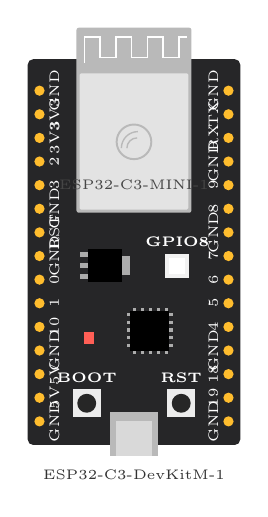
\begin{tikzpicture}
    \pic at (0,0) {esp32c3};
    \node[font=\tiny, text=gray!40!black, anchor=north] at (1.35,-0.2) {ESP32-C3-DevKitM-1};
  \end{tikzpicture}}

% ---------- Wokwi window (schematic; replace with a screenshot if you like) ----------
\newcommand{\wokwiwindow}{%
  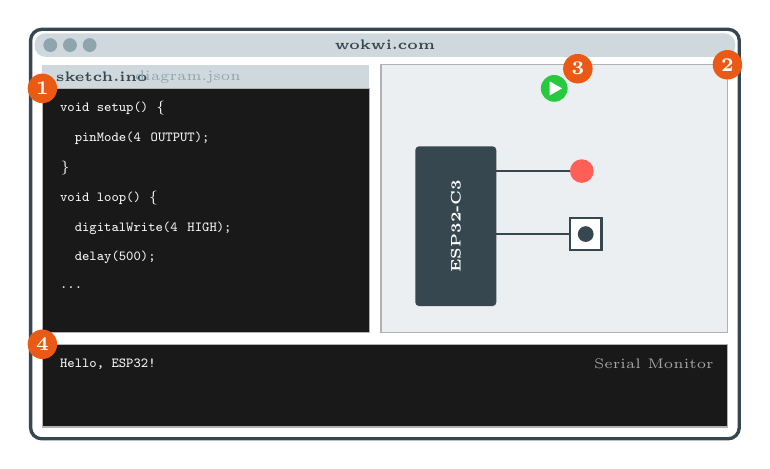
\begin{tikzpicture}[font=\tiny]
    \draw[nInk, very thick, fill=white, rounded corners=4pt] (0,0) rectangle (9,5.2);
    \fill[nLight, rounded corners=4pt] (0.05,4.85) rectangle (8.95,5.15);
    \fill[nLine] (0.25,5.0) circle (2.5pt); \fill[nLine] (0.5,5.0) circle (2.5pt); \fill[nLine] (0.75,5.0) circle (2.5pt);
    \node[font=\tiny\bfseries, text=nInk] at (4.5,5.0) {wokwi.com};
    % code editor
    \fill[nLight] (0.15,4.45) rectangle (4.3,4.75);
    \node[anchor=west, font=\tiny\bfseries, text=nInk] at (0.2,4.6) {sketch.ino};
    \node[anchor=west, font=\tiny, text=nLine] at (1.2,4.6) {diagram.json};
    \draw[gray!60, fill=VSDarkBg] (0.15,1.35) rectangle (4.3,4.45);
    \foreach \t [count=\j from 0] in {void setup() \{, \ \ pinMode(4\, OUTPUT);, \}, void loop() \{, \ \ digitalWrite(4\, HIGH);, \ \ delay(500);, \ldots}
      \node[anchor=west, text=VSText, font=\ttfamily\tiny] at (0.25,{4.2-0.38*\j}) {\t};
    % diagram
    \draw[gray!60, fill=nFill] (4.45,1.35) rectangle (8.85,4.75);
    \fill[MacGreen] (6.65,4.45) circle (0.17);
    \fill[white] (6.59,4.36) -- (6.59,4.54) -- (6.75,4.45) -- cycle;
    \draw[nInk, thick, fill=nInk, rounded corners=1pt] (4.9,1.7) rectangle (5.9,3.7);
    \node[font=\tiny\bfseries, text=white, rotate=90] at (5.4,2.7) {ESP32-C3};
    \fill[MacRed] (7.0,3.4) circle (0.15);
    \draw[nInk, thick] (5.9,3.4) -- (6.85,3.4);
    \draw[nInk, thick, fill=white] (6.85,2.4) rectangle (7.25,2.8);
    \fill[nInk] (7.05,2.6) circle (0.1);
    \draw[nInk, thick] (5.9,2.6) -- (6.85,2.6);
    % serial monitor
    \draw[gray!60, fill=VSDarkBg] (0.15,0.15) rectangle (8.85,1.2);
    \node[anchor=west, text=VSText, font=\ttfamily\tiny] at (0.25,0.95) {Hello, ESP32!};
    \node[anchor=east, font=\tiny, text=gray!70] at (8.8,0.95) {Serial Monitor};
    % badges
    \foreach \x/\y/\n in {0.15/4.45/1, 8.85/4.75/2, 6.95/4.7/3, 0.15/1.2/4}
      \node[circle, fill=AccentOrange, text=white, font=\bfseries\scriptsize, inner sep=1.5pt] at (\x,\y) {\n};
  \end{tikzpicture}}

% ---------- our circuit for today ----------
\newcommand{\ourcircuit}{%
  \begin{tikzpicture}[>=Stealth, font=\scriptsize]
    \node[draw=nInk, very thick, fill=nInk, text=white, rounded corners=3pt, minimum width=2.0cm,
      minimum height=3.2cm, font=\scriptsize\bfseries, align=center] (esp) at (0,0) {ESP32-C3};
    \node[lbox, draw=nLine, fill=nFill, text=nInk, minimum width=1.9cm] (led) at (4.2,1.2) {\faLightbulb\ LED};
    \node[lbox, draw=nInk, fill=nFill, minimum width=1.9cm] (ba) at (4.2,0.4) {\faDotCircle\ Button A};
    \node[lbox, draw=nInk, fill=nFill, minimum width=1.9cm] (bb) at (4.2,-0.4) {\faDotCircle\ Button B};
    \node[lbox, draw=nLine, fill=nFill, text=nInk, minimum width=1.9cm] (lcd) at (4.2,-1.25) {\faTv\ LCD 16$\times$2};
    \draw[very thick, nInk] (esp.east |- led) -- node[above, font=\tiny] {GPIO 4} (led);
    \draw[very thick, nInk] (esp.east |- ba) -- node[above, font=\tiny] {GPIO 5} (ba);
    \draw[very thick, nInk] (esp.east |- bb) -- node[above, font=\tiny] {GPIO 6} (bb);
    \draw[very thick, nInk] (esp.east |- lcd) -- node[above, font=\tiny] {GPIO 8, 9 (I2C)} (lcd);
  \end{tikzpicture}}

% ---------- Wokwi-style parts for the "Build it" slides ----------
\definecolor{PcbBlack}{RGB}{38,38,40}
\definecolor{ResBody}{RGB}{214,184,140}
\definecolor{LcdScreen}{RGB}{131,190,40}
\definecolor{WireGreen}{RGB}{0,140,40}
\newcommand{\pinfont}{\fontsize{3.4}{3.6}\selectfont}
\tikzset{
  % a wire; the white edge makes crossings easy to see
  wire/.style={line width=1.1pt, rounded corners=1.5pt, preaction={draw, white, line width=2.6pt}},
  % ESP32-C3-DevKitM-1 as in Wokwi (USB at the bottom); pins (-L0)..(-L14), (-R0)..(-R14), 0 = top
  pics/esp32c3/.style={code={
    \fill[PcbBlack, rounded corners=2pt] (0,0) rectangle (2.7,4.9);
    % module ESP32-C3-MINI-1: the antenna part sticks out above the board
    \fill[gray!55, rounded corners=0.8pt] (0.62,2.95) rectangle (2.08,5.3);
    \draw[white, line width=0.5pt] (0.72,4.85) -- (0.72,5.18)
      \foreach \i in {1,...,3} { -- ++(0.2,0) -- ++(0,-0.26) -- ++(0.2,0) -- ++(0,0.26) } -- ++(0.1,0);
    \fill[gray!22, rounded corners=0.5pt] (0.66,2.99) rectangle (2.04,4.72);
    \draw[gray!55, line width=0.7pt] (1.35,3.85) circle (0.22);
    \draw[gray!55, line width=0.5pt] (1.26,3.77) arc (180:90:0.13) (1.19,3.77) arc (180:90:0.21);
    \node[font=\pinfont, text=gray!55!black] at (1.35,3.3) {ESP32-C3-MINI-1};
    % voltage regulator: 3 small legs on the left, a wide tab on the right
    \foreach \y in {2.14,2.28,2.42} \fill[gray!65] (0.66,\y-0.03) rectangle (0.76,\y+0.03);
    \fill[gray!65] (1.18,2.16) rectangle (1.3,2.4);
    \fill[black] (0.76,2.07) rectangle (1.2,2.49);
    % RGB LED on GPIO 8
    \fill[gray!10] (1.75,2.12) rectangle (2.05,2.42);
    \fill[white] (1.8,2.17) rectangle (2.0,2.37);
    \node[font=\pinfont\bfseries\rmfamily, text=white] at (1.9,2.58) {GPIO8};
    % USB-to-serial chip with pins on all sides
    \foreach \i in {0,...,4} {
      \fill[gray!65] ({1.34+0.1*\i},1.16) rectangle ++(0.04,0.05);
      \fill[gray!65] ({1.34+0.1*\i},1.69) rectangle ++(0.04,0.05);
      \fill[gray!65] (1.26,{1.24+0.1*\i}) rectangle ++(0.05,0.04);
      \fill[gray!65] (1.79,{1.24+0.1*\i}) rectangle ++(0.05,0.04);
    }
    \fill[black] (1.3,1.2) rectangle (1.8,1.7);
    % power LED
    \fill[MacRed] (0.72,1.28) rectangle (0.84,1.44);
    % BOOT and RST buttons
    \foreach \x/\t in {0.75/BOOT,1.95/RST} {
      \fill[gray!15] (\x-0.18,0.35) rectangle (\x+0.18,0.71);
      \fill[black!85] (\x,0.53) circle (0.12);
      \node[font=\pinfont\bfseries\rmfamily, text=white] at (\x,0.86) {\t};
    }
    % USB connector, sticks out below the board
    \fill[gray!55] (1.05,-0.14) rectangle (1.65,0.42);
    \fill[gray!30] (1.12,-0.14) rectangle (1.58,0.3);
    \foreach \n [count=\k from 0] in {GND,3V3,3V3,2,3,GND,RST,GND,0,1,10,GND,5V,5V,GND} {
      \fill[MacYellow] (0.15,{4.5-0.3*\k}) circle (0.065);
      \node[rotate=90, font=\pinfont, text=white] at (0.34,{4.5-0.3*\k}) {\n};
      \coordinate (-L\k) at (0.15,{4.5-0.3*\k});
    }
    \foreach \n [count=\k from 0] in {GND,TX,RX,GND,9,8,GND,7,6,5,4,GND,18,19,GND} {
      \fill[MacYellow] (2.55,{4.5-0.3*\k}) circle (0.065);
      \node[rotate=90, font=\pinfont, text=white] at (2.36,{4.5-0.3*\k}) {\n};
      \coordinate (-R\k) at (2.55,{4.5-0.3*\k});
    }
  }},
  % red LED, origin = middle of the rim; legs (-C) straight, (-A) bent
  pics/wled/.style={code={
    \draw[gray!60, line width=0.9pt] (-0.09,0) -- (-0.09,-0.42);
    \draw[gray!60, line width=0.9pt] (0.09,0) -- (0.09,-0.12) -- (0.17,-0.2) -- (0.17,-0.42);
    \fill[MacRed!80!black] (-0.24,0) rectangle (0.24,0.07);
    \fill[MacRed] (-0.2,0.07) -- (-0.2,0.32) arc (180:0:0.2) -- (0.2,0.07) -- cycle;
    \fill[white, opacity=0.45] (-0.1,0.38) ellipse (0.04 and 0.1);
    \node[font=\pinfont, text=black, anchor=east] at (-0.1,-0.3) {C};
    \node[font=\pinfont, text=black, anchor=west] at (0.18,-0.3) {A};
    \coordinate (-C) at (-0.09,-0.42);
    \coordinate (-A) at (0.17,-0.42);
  }},
  % 220 ohm resistor, vertical; origin = bottom lead (-2), top lead (-1)
  pics/wres/.style={code={
    \draw[gray!60, line width=0.9pt] (0,0) -- (0,0.85);
    \fill[ResBody, rounded corners=0.8pt] (-0.09,0.15) rectangle (0.09,0.7);
    \foreach \y/\c in {0.6/red, 0.52/red, 0.44/brown!80!black, 0.24/MacYellow!70!brown}
      \fill[\c] (-0.09,\y) rectangle (0.09,\y+0.05);
    \coordinate (-1) at (0,0.85);
    \coordinate (-2) at (0,0);
  }},
  % pushbutton, origin = centre; legs (-1l), (-2l), (-1r), (-2r); argument = colour of the cap
  pics/wbutton/.style={code={
    \foreach \x in {-1,1} \foreach \y in {-1,1}
      \draw[gray!60, line width=0.9pt] (0.3*\x,0.13*\y) -- (0.4*\x,0.13*\y);
    \fill[black!80, rounded corners=1pt] (-0.3,-0.25) rectangle (0.3,0.25);
    \fill[gray!35] (-0.25,-0.2) rectangle (0.25,0.2);
    \fill[#1] (0,0) circle (0.14);
    \node[font=\pinfont, text=black, anchor=south east] at (-0.33,0.13) {1.l};
    \node[font=\pinfont, text=black, anchor=north west] at (0.33,-0.13) {2.r};
    \node[font=\pinfont, text=black, anchor=north east] at (-0.33,-0.13) {2.l};
    \node[font=\pinfont, text=black, anchor=south west] at (0.33,0.13) {1.r};
    \coordinate (-1l) at (-0.4,0.13);  \coordinate (-2l) at (-0.4,-0.13);
    \coordinate (-1r) at (0.4,0.13);   \coordinate (-2r) at (0.4,-0.13);
  }},
  % LCD 16x2 with I2C, origin = bottom left; pins (-GND), (-VCC), (-SDA), (-SCL) on the left edge
  pics/wlcd/.style={code={
    \fill[mygreen!55!black, rounded corners=1.5pt] (0,0) rectangle (3.0,1.2);
    \fill[black!85] (0.55,0.12) rectangle (2.9,1.08);
    \fill[LcdScreen] (0.62,0.2) rectangle (2.83,1.0);
    \foreach \r in {0,1} \foreach \c in {0,...,15}
      \fill[LcdScreen!85!black] ({0.66+0.135*\c},{0.26+0.38*\r}) rectangle ++(0.11,0.3);
    \foreach \n [count=\k from 0] in {GND,VCC,SDA,SCL} {
      \fill[MacYellow] (0.14,{1.0-0.2*\k}) circle (0.055);
      \node[font=\pinfont, text=white, anchor=west] at (0.2,{1.0-0.2*\k}) {\n};
      \coordinate (-\n) at (0.14,{1.0-0.2*\k});
    }
  }},
}

% the circuit of the day, built in 4 steps: #1 = step (1 LED, 2 button A, 3 LCD, 4 button B)
% parts of the current step are drawn normally, parts of earlier steps are faded
\newcommand{\buildopacity}[2]{\ifnum#1>#2 0.3\else 1\fi}
\newcommand{\buildpic}[1]{%
  \begin{tikzpicture}[font=\tiny]
    \useasboundingbox (-0.45,-0.2) rectangle (7.3,5.7);
    \pic (esp) at (0,0) {esp32c3};
    % step 1: LED and resistor, GND along the bottom
    \begin{scope}[opacity=\buildopacity{#1}{1}]
      \pic (res) at (4.91,0.65) {wres};
      \pic (led) at (5.0,1.95) {wled};
      \draw[wire, black] (esp-R14) -- (4.91,0.3) -- (res-2);
      \draw[wire, WireGreen] (res-1) -- (led-C);
      \draw[wire, WireGreen] (esp-R10) -| (4.25,0.48) -| (led-A);
      \node[font=\fontsize{5.5}{6}\selectfont\bfseries, anchor=east] at (4.83,1.05) {220\,$\Omega$};
    \end{scope}
    % step 2: button A
    \ifnum#1>1
    \begin{scope}[opacity=\buildopacity{#1}{2}]
      \pic (ba) at (4.9,2.85) {wbutton=MacGreen};
      \node[font=\scriptsize\bfseries, anchor=south] at (4.9,3.1) {A};
      \draw[wire, black] (ba-2r) -| (5.75,0.3) -- (4.91,0.3);
      \draw[wire, WireGreen] (esp-R9) -| ([xshift=-0.35cm]ba-1l) -- (ba-1l);
    \end{scope}
    \fi
    % step 3: LCD (I2C)
    \ifnum#1>2
    \begin{scope}[opacity=\buildopacity{#1}{3}]
      \pic (lcd) at (4.2,4.2) {wlcd};
      \draw[wire, black] (esp-R0) -| ([xshift=-1.09cm]lcd-GND) -- (lcd-GND);
      \draw[wire, StorageBlue] (esp-R5) -| ([xshift=-0.59cm]lcd-SDA) -- (lcd-SDA);
      \draw[wire, ProgramPurple] (esp-R4) -| ([xshift=-0.79cm]lcd-SCL) -- (lcd-SCL);
      \draw[wire, MacRed] (esp-L12) -- (-0.35,0.9) -- (-0.35,5.6) -- (4.0,5.6) |- (lcd-VCC);
    \end{scope}
    \fi
    % step 4: button B
    \ifnum#1>3
    \begin{scope}[opacity=\buildopacity{#1}{4}]
      \pic (bb) at (4.9,3.75) {wbutton=StorageBlue};
      \node[font=\scriptsize\bfseries, anchor=south] at (4.9,4.0) {B};
      \draw[wire, black] (bb-2r) -| (5.75,2.72);
      \fill (5.75,2.72) circle (0.05);
      \draw[wire, WireGreen] (esp-R8) -| ([xshift=-0.55cm]bb-1l) -- (bb-1l);
    \end{scope}
    \fi
  \end{tikzpicture}}

% ---------- power: VCC, GND and a closed loop ----------
\newcommand{\powerexplain}{%
  \begin{tikzpicture}[font=\scriptsize, >=Stealth]
    % rails
    \draw[line width=2pt, nInk] (0,2.0) -- (4.6,2.0);
    \node[anchor=west, font=\scriptsize\bfseries, text=nInk, align=left] at (4.7,2.0) {VCC (+)\\[-1pt]{\tiny 3V3 = 3.3\,V, 5V = 5\,V}};
    \draw[line width=2pt, black] (0,-1.0) -- (4.6,-1.0);
    \node[anchor=west, font=\scriptsize\bfseries, align=left] at (4.7,-1.0) {GND ($-$)\\[-1pt]{\tiny 0\,V}};
    % voltage between the rails
    \draw[<->, thick, DeepBlue] (-0.4,-1.0) -- node[left, font=\scriptsize\bfseries, align=center] {voltage\\3.3\,V} (-0.4,2.0);
    % a part between the rails: resistor + LED
    \draw[thick] (1.2,2.0) -- (1.2,1.55);
    \draw[thick, fill=ResBody] (1.08,1.55) rectangle (1.32,0.85);
    \draw[thick] (1.2,0.85) -- (1.2,0.6);
    \draw[thick, fill=nFill] (0.95,0.6) -- (1.45,0.6) -- (1.2,0.15) -- cycle;
    \draw[very thick] (0.95,0.15) -- (1.45,0.15);
    \foreach \d in {0,0.15} \draw[->, nInk, thick] (1.5,{0.45-\d}) -- ++(0.28,0.16);
    \draw[thick] (1.2,0.15) -- (1.2,-1.0);
    \fill[nInk] (1.2,2.0) circle (0.06);  \fill (1.2,-1.0) circle (0.06);
    \draw[->, line width=1.4pt, AccentOrange] (0.65,1.8) -- node[sloped, above, font=\tiny\bfseries] {current} (0.65,-0.8);
    \node[font=\tiny\bfseries, aExec, align=center] at (1.2,-1.4) {\faCheck\ closed loop:\\+ $\to$ part $\to$ GND};
    % a short circuit
    \draw[line width=1.4pt, aWrite] (3.6,2.0) -- (3.6,-1.0);
    \fill[nInk] (3.6,2.0) circle (0.06);  \fill (3.6,-1.0) circle (0.06);
    \node[font=\Large\bfseries, text=aWrite, fill=white, inner sep=1pt] at (3.6,0.5) {\faTimes};
    \node[font=\tiny\bfseries, aWrite, align=center] at (3.6,-1.4) {\faTimes\ short circuit:\\VCC straight to GND};
  \end{tikzpicture}}

% ---------- how an LED works: the part and its circuit ----------
\newcommand{\ledexplain}{%
  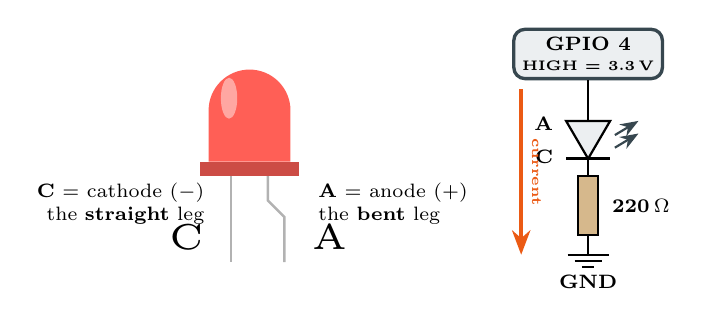
\begin{tikzpicture}[font=\scriptsize, >=Stealth]
    \begin{scope}[scale=2.6, transform shape]
      \pic (bl) at (0,0) {wled};
    \end{scope}
    \node[anchor=west, align=left] (la) at (0.75,-0.35) {\textbf{A} = anode (+)\\the \textbf{bent} leg};
    \node[anchor=east, align=right] (lc) at (-0.45,-0.35) {\textbf{C} = cathode ($-$)\\the \textbf{straight} leg};
    % the circuit
    \begin{scope}[xshift=4.3cm, yshift=-0.2cm]
      \node[lbox, draw=nInk, fill=nFill] (gpio) at (0,1.75) {GPIO 4\\[-1pt]{\tiny HIGH = 3.3\,V}};
      \draw[thick] (gpio.south) -- (0,0.9);
      \draw[thick, fill=nFill] (-0.28,0.9) -- (0.28,0.9) -- (0,0.42) -- cycle;
      \draw[very thick] (-0.28,0.42) -- (0.28,0.42);
      \foreach \d in {0,0.16} \draw[->, nInk, thick] (0.34,{0.72-\d}) -- ++(0.3,0.18);
      \node[anchor=east, font=\scriptsize\bfseries] at (-0.32,0.86) {A};
      \node[anchor=east, font=\scriptsize\bfseries] at (-0.32,0.44) {C};
      \draw[thick] (0,0.42) -- (0,0.2);
      \draw[thick, fill=ResBody] (-0.13,0.2) rectangle (0.13,-0.55);
      \node[anchor=west, font=\scriptsize\bfseries] at (0.18,-0.18) {220\,$\Omega$};
      \draw[thick] (0,-0.55) -- (0,-0.8);
      \foreach \w/\y in {0.26/-0.8, 0.17/-0.88, 0.08/-0.96} \draw[thick] (-\w,\y) -- (\w,\y);
      \node[font=\scriptsize\bfseries] at (0,-1.15) {GND};
      \draw[->, line width=1.3pt, AccentOrange] (-0.85,1.3) -- node[sloped, above, font=\tiny\bfseries] {current} (-0.85,-0.8);
    \end{scope}
  \end{tikzpicture}}

% ---------- how a pushbutton works: 4 legs, 2 pairs ----------
% #1 = 0 not pressed, 1 pressed
\newcommand{\buttoninside}[1]{%
  \begin{tikzpicture}[font=\tiny, >=Stealth]
    \foreach \x/\y/\n in {0/0.8/1.l, 1.6/0.8/1.r, 0/0/2.l, 1.6/0/2.r} {
      \fill[gray!60] (\x,\y) circle (0.06);
      \node[font=\tiny\bfseries, anchor=\ifdim\x pt<1pt east\else west\fi] at (\x,\y) {\n};
    }
    \draw[thick] (0,0.8) -- (1.6,0.8);
    \draw[thick] (0,0) -- (1.6,0);
    \fill (0.8,0.8) circle (0.04);  \fill (0.8,0) circle (0.04);
    \ifnum#1=0
      \draw[thick] (0.8,0.8) -- (0.8,0.62) -- (1.1,0.22);
      \draw[thick] (0.8,0) -- (0.8,0.18);
    \else
      \draw[line width=1.6pt, nInk] (0.8,0.8) -- (0.8,0);
    \fi
  \end{tikzpicture}}
\newcommand{\buttonexplain}{%
  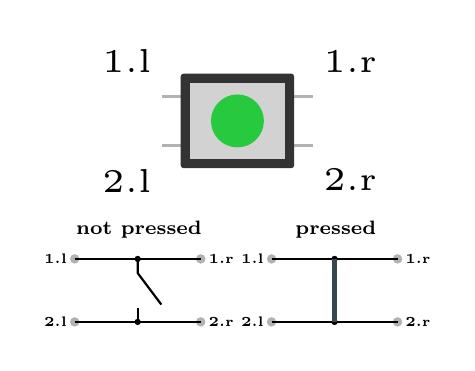
\begin{tikzpicture}[font=\scriptsize]
    \begin{scope}[scale=2.4, transform shape]
      \pic (bx) at (0,0) {wbutton=MacGreen};
    \end{scope}
    \node[anchor=north, align=center] at (-1.25,-1.15) {\textbf{not pressed}\\[2pt]\buttoninside{0}};
    \node[anchor=north, align=center] at (1.25,-1.15) {\textbf{pressed}\\[2pt]\buttoninside{1}};
  \end{tikzpicture}}

% ---------- I2C: one controller, many devices on 2 wires ----------
\newcommand{\itwocbus}{%
  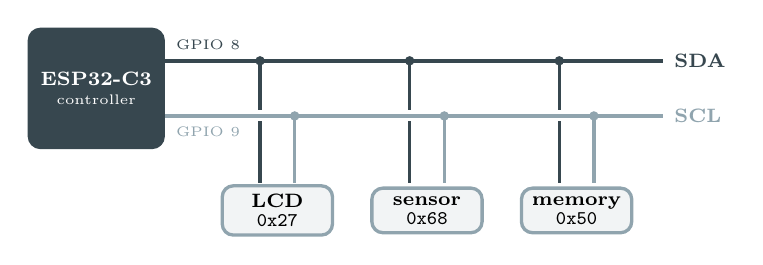
\begin{tikzpicture}[font=\scriptsize, >=Stealth]
    \node[lbox, draw=nInk, fill=nInk, text=white, minimum width=1.7cm, minimum height=1.5cm]
      (cpu) at (0,0) {ESP32-C3\\[-1pt]{\tiny\mdseries controller}};
    \draw[line width=1.5pt, nInk] (cpu.east |- 0,0.35) node[above right, font=\tiny] {GPIO 8} -- (7.2,0.35)
      node[right, font=\scriptsize\bfseries] {SDA};
    \foreach \x/\n/\a/\c in {2.3/LCD/0x27/nLine, 4.2/sensor/0x68/nLine, 6.1/memory/0x50/nLine} {
      \draw[line width=1.2pt, nInk] (\x-0.22,0.35) -- (\x-0.22,-1.2);
      \fill[nInk] (\x-0.22,0.35) circle (0.06);
      \node[lbox, draw=\c, fill=\c!12, minimum width=1.4cm] at (\x,-1.55) {\n\\[-1pt]\texttt{\a}};
    }
    \draw[line width=1.5pt, nLine, preaction={draw, white, line width=4pt}] (cpu.east |- 0,-0.35)
      node[below right, font=\tiny] {GPIO 9} -- (7.2,-0.35) node[right, font=\scriptsize\bfseries] {SCL};
    \foreach \x in {2.3,4.2,6.1} {
      \draw[line width=1.2pt, nLine] (\x+0.22,-0.35) -- (\x+0.22,-1.2);
      \fill[nLine] (\x+0.22,-0.35) circle (0.06);
    }
  \end{tikzpicture}}

% ---------- one I2C message on the wires: #1 = the step to highlight (1..6) ----------
\newcommand{\itwoctiming}[1]{%
  \begin{tikzpicture}[font=\scriptsize, >=Stealth]
    % the steps: highlighted band and a label on top
    \foreach \n/\a/\b/\t/\c in {1/0.3/1.0/START/AccentOrange, 2/1.0/5.0/{address \texttt{0x27} + write}/AccentOrange,
        3/5.0/5.5/ACK/AccentOrange, 4/5.5/9.5/{data byte}/AccentOrange, 5/9.5/10.0/ACK/AccentOrange, 6/10.0/10.75/STOP/AccentOrange} {
      \ifnum\n=#1
        \fill[\c!18, rounded corners=2pt] (\a,-1.55) rectangle (\b,1.45);
        \node[font=\scriptsize\bfseries, text=\c!80!black] at ({(\a+\b)/2},1.25) {\t};
      \else
        \node[font=\tiny, text=gray] at ({(\a+\b)/2},1.25) {\t};
      \fi
      \draw[gray!40, densely dotted] (\a,-1.55) -- (\a,1.1);
    }
    \node[anchor=east, font=\scriptsize\bfseries, text=nInk] at (-0.1,0.6) {SCL};
    \node[anchor=east, font=\scriptsize\bfseries, text=nInk] at (-0.1,-0.6) {SDA};
    % SCL: high, falls after START, 18 clock ticks, high again before STOP
    \draw[thick, nInk] (0,0.9) -- (0.8,0.9) -- (0.8,0.3) -- (1.25,0.3)
      \foreach \k in {0,...,17} { -- ({1.25+0.5*\k},0.9) -- ({1.5+0.5*\k},0.9) -- ({1.5+0.5*\k},0.3) -- ({1.75+0.5*\k},0.3) }
      -- (10.2,0.3) -- (10.2,0.9) -- (10.9,0.9);
    % SDA: falls at START, one bit per tick, rises at STOP
    \draw[thick, nInk] (0,-0.3) -- (0.5,-0.3) -- (0.5,-0.9) -- (1.0,-0.9);
    \foreach \x/\p/\v/\c in {1.0/0/0/nInk, 1.5/0/1/nInk, 2.0/1/0/nInk, 2.5/0/0/nInk, 3.0/0/1/nInk, 3.5/1/1/nInk, 4.0/1/1/nInk, 4.5/1/0/nInk, 5.0/0/0/nInk, 5.5/0/0/nInk, 6.0/0/1/nInk, 6.5/1/0/nInk, 7.0/0/0/nInk, 7.5/0/1/nInk, 8.0/1/0/nInk, 8.5/0/0/nInk, 9.0/0/0/nInk, 9.5/0/0/nInk}
      \draw[thick, \c] (\x,{-0.9+0.6*\p}) -- (\x,{-0.9+0.6*\v}) -- (\x+0.5,{-0.9+0.6*\v});
    \draw[thick, nInk] (10.0,-0.9) -- (10.45,-0.9) -- (10.45,-0.3) -- (10.9,-0.3);
    \foreach \x/\v in {1.25/0, 1.75/1, 2.25/0, 2.75/0, 3.25/1, 3.75/1, 4.25/1, 4.75/0, 5.25/0, 5.75/0, 6.25/1, 6.75/0, 7.25/0, 7.75/1, 8.25/0, 8.75/0, 9.25/0, 9.75/0} \node[font=\tiny, text=gray!70!black] at (\x,-1.2) {\v};
    \node[font=\tiny, text=gray!70!black] at (4.75,-1.42) {W};
  \end{tikzpicture}}

% ---------- showcase: Snake on a Nokia 5110 screen with a joystick ----------
\newcommand{\snakeshowcase}{%
  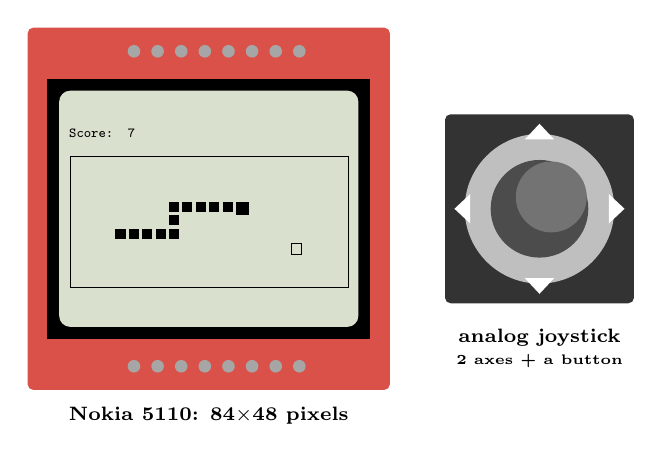
\begin{tikzpicture}[font=\scriptsize]
    % the Nokia 5110 module
    \fill[MacRed!85!black, rounded corners=2pt] (0,0) rectangle (4.6,4.6);
    \foreach \i in {0,...,7} {
      \fill[gray!70] ({1.35+0.3*\i},0.3) circle (0.08);
      \fill[gray!70] ({1.35+0.3*\i},4.3) circle (0.08);
    }
    \fill[black] (0.25,0.65) rectangle (4.35,3.95);
    \fill[LcdScreen!40!gray!30, rounded corners=4pt] (0.4,0.8) rectangle (4.2,3.8);
    % the game: 84 x 48 pixels drawn at 0.0425 cm per pixel
    \begin{scope}[shift={(0.52,3.32)}, x=0.0425cm, y=-0.0425cm]
      \node[anchor=north west, inner sep=0, font=\ttfamily\bfseries\tiny] at (0,0) {Score: 7};
      \draw[line width=0.3pt] (0.5,8.5) rectangle (83.5,47.5);
      \foreach \x/\y in {3/5,4/5,5/5,6/5,7/5,7/4,7/3,8/3,9/3,10/3,11/3} \fill ({2+4*\x},{10+4*\y}) rectangle ++(3,3);
      \fill ({2+4*12},{10+4*3}) rectangle ++(4,4);
      \draw[line width=0.3pt] ({2+4*16+0.5},{10+4*6+0.5}) rectangle ++(3,3);
    \end{scope}
    \node[font=\scriptsize\bfseries, anchor=north] at (2.3,-0.1) {Nokia 5110: 84$\times$48 pixels};
    % the joystick
    \begin{scope}[shift={(5.3,1.1)}]
      \fill[black!80, rounded corners=2pt] (0,0) rectangle (2.4,2.4);
      \fill[gray!50] (1.2,1.2) circle (0.95);
      \fill[black!70] (1.2,1.2) circle (0.62);
      \fill[black!55] (1.35,1.35) circle (0.45);
      \foreach \a in {0,90,180,270} \fill[white] ([shift={(\a:1.08)}]1.2,1.2) -- ([shift={(\a+12:0.9)}]1.2,1.2) -- ([shift={(\a-12:0.9)}]1.2,1.2) -- cycle;
      \node[font=\scriptsize\bfseries, anchor=north, align=center] at (1.2,-0.2) {analog joystick\\{\tiny 2 axes + a button}};
    \end{scope}
  \end{tikzpicture}}

% ---------- inside the ESP32-C3: CPU, internal bus, controllers; pins and wires outside ----------
% #1 = 0 overview, 1 address on the bus, 2 GPIO recognises it, 3 data written: the LED lights up
\newcommand{\chipbus}[1]{%
  \begin{tikzpicture}[>=Stealth, font=\scriptsize]
    % the chip
    \draw[nLine, very thick, dashed, rounded corners=6pt] (-1.3,-1.6) rectangle (11.9,2.5);
    \node[anchor=north west, font=\scriptsize\bfseries, text=nInk] at (-1.2,2.45) {\faMicrochip\ inside the ESP32-C3 chip};
    \node[cpubox, minimum width=1.8cm, minimum height=0.9cm] (cpu) at (0.4,1.45) {CPU};
    % the internal bus
    \ifnum#1>0 \def\buswidth{1.5pt}\else \def\buswidth{2pt}\fi
    \foreach \y/\c/\t in {0.75/nInk/address, 0.45/nLine/data, 0.15/nLight/control} {
      \draw[line width=\buswidth, \c] (0.4,\y) -- (10.4,\y);
      \node[anchor=west, font=\tiny\bfseries, text=\c] at (10.45,\y) {\t};
    }
    \node[font=\tiny\bfseries, text=nInk, anchor=south] at (5.4,0.78) {internal bus};
    \draw[very thick, nInk] (cpu.south) -- (0.4,0.15);
    % memory and controllers
    \node[rambox, minimum width=2.0cm, minimum height=0.85cm] (mem) at (2.9,-0.75) {Memory\\[-1pt]{\tiny\mdseries RAM, flash}};
    \node[iobox, minimum width=2.0cm, minimum height=0.85cm] (gpio) at (6.0,-0.75) {GPIO controller\\[-1pt]{\tiny\mdseries \texttt{0x6000\,4000}}};
    \node[iobox, minimum width=2.0cm, minimum height=0.85cm] (i2c) at (9.1,-0.75) {I2C controller\\[-1pt]{\tiny\mdseries \texttt{0x6001\,3000}}};
    \foreach \n in {mem,gpio,i2c} \draw[very thick, nInk] (\n.north) -- (\n.north |- 0,0.75);
    % every connection reaches all three groups of lines: address, data and control
    \foreach \x in {0.4,2.9,6.0,9.1}
      \foreach \y/\c in {0.75/nInk, 0.45/nLine, 0.15/nLight}
        \fill[\c] (\x,\y) circle (0.075);
    % pins on the edge of the chip, wires on the board
    \foreach \x/\l/\n in {5.6/4/gpio, 6.4/5/gpio, 8.7/8/i2c, 9.5/9/i2c} {
      \draw[thick, gray!70!black] (\x,-1.175) -- (\x,-1.6);
      \fill[MacYellow] (\x-0.09,-1.69) rectangle (\x+0.09,-1.51);
      \node[font=\tiny\bfseries, anchor=west] at (\x+0.08,-1.4) {\l};
    }
    \draw[line width=1.2pt, WireGreen] (5.6,-1.69) -- (5.6,-2.25);
    \draw[line width=1.2pt, WireGreen] (6.4,-1.69) -- (6.4,-2.25);
    \draw[line width=1.2pt, nInk] (8.7,-1.69) -- (8.7,-2.2);
    \draw[line width=1.2pt, nLine] (9.5,-1.69) -- (9.5,-2.2);
    \ifnum#1=3
      \fill[nLight] (5.6,-2.5) circle (0.38);
      \fill[nInk] (5.6,-2.5) circle (0.24);
      \node[font=\tiny\bfseries, text=nInk, anchor=east] at (5.5,-1.95) {3.3\,V};
    \else
      \fill[white] (5.6,-2.5) circle (0.24); \draw[nLine] (5.6,-2.5) circle (0.24);
    \fi
    \node[font=\tiny, anchor=north] at (5.6,-2.78) {LED};
    \fill[black!75, rounded corners=1pt] (6.2,-2.7) rectangle (6.6,-2.3);  \fill[MacGreen] (6.4,-2.5) circle (0.12);
    \node[font=\tiny, anchor=north] at (6.4,-2.78) {button};
    \node[lbox, draw=nLine, fill=nFill, text=nInk, minimum width=1.6cm] (lcd) at (9.1,-2.55) {LCD\\[-1pt]{\tiny\mdseries I2C address \texttt{0x27}}};
    \node[font=\tiny, text=gray!40!black, anchor=west, align=left] at (10.05,-1.95) {SDA, SCL:\\2 wires};
    \node[font=\scriptsize\bfseries, text=gray!40!black, anchor=west] at (-1.2,-2.2) {on the board: real wires};
    % the steps of one store: sw to 0x6000 4008
    \ifnum#1>0
      \node[font=\tiny\ttfamily, fill=white, draw=nInk, rounded corners=1pt, anchor=west] at (1.5,1.45) {sw a4, 8(a5)};
      \node[font=\tiny\bfseries\ttfamily, fill=white, draw=nLine, rounded corners=1pt] at (1.8,0.75) {0x6000\,4008};
    \fi
    \ifnum#1>1
      \draw[line width=1.6pt, AccentOrange, rounded corners=3pt] ([shift={(-0.08,-0.08)}]gpio.south west) rectangle ([shift={(0.08,0.08)}]gpio.north east);
      \node[font=\tiny\bfseries, text=AccentOrange, anchor=south west] at ([xshift=0.05cm]gpio.north east) {mine!};
      \node[font=\tiny, text=gray, anchor=south west] at ([xshift=0.05cm]mem.north east) {not mine};
      \node[font=\tiny, text=gray, anchor=south west] at ([xshift=0.05cm]i2c.north east) {not mine};
    \fi
    \ifnum#1>2
      \node[font=\tiny\bfseries\ttfamily, fill=white, draw=nLine, rounded corners=1pt] at (1.8,0.45) {0x10 = bit 4};
      \node[font=\tiny\bfseries, fill=white, awrite, rounded corners=1pt] at (1.8,0.15) {write};
    \fi
  \end{tikzpicture}}

% ---------- lcd.print: CPU -> I2C controller (internal bus) -> LCD (2 wires) ----------
\newcommand{\twobuses}{%
  \begin{tikzpicture}[>=Stealth, font=\scriptsize]
    \draw[nLine, very thick, dashed, rounded corners=6pt] (-0.3,-0.75) rectangle (5.3,1.2);
    \node[anchor=north west, font=\tiny\bfseries, text=nInk] at (-0.25,1.17) {\faMicrochip\ inside the chip};
    \node[cpubox, minimum width=1.4cm, minimum height=0.8cm] (cpu) at (0.6,0.1) {CPU};
    \node[iobox, minimum width=1.8cm, minimum height=0.8cm] (ctl) at (4.1,0.1) {I2C\\[-1pt]controller};
    \draw[->, line width=1.8pt, nInk] (cpu.east) -- node[above, font=\tiny\bfseries] {internal bus} node[below, font=\tiny\ttfamily] {sw \ldots\ 0x6001\,3xxx} (ctl.west);
    \node[lbox, draw=nLine, fill=nFill, text=nInk, minimum width=1.4cm, minimum height=0.8cm] (lcd) at (7.3,0.1) {LCD\\[-1pt]{\tiny\mdseries \texttt{0x27}}};
    \draw[->, line width=1.2pt, nInk] ([yshift=0.12cm]ctl.east) -- ([yshift=0.12cm]lcd.west);
    \draw[line width=1.2pt, nLine] ([yshift=-0.12cm]ctl.east) -- ([yshift=-0.12cm]lcd.west);
    \node[font=\tiny\bfseries, anchor=south] at (6.05,0.25) {SDA, SCL};
    \node[font=\tiny, anchor=north, align=center] at (6.05,-0.05) {START, \texttt{0x27},\\data, STOP};
    \node[font=\tiny\bfseries, text=gray!40!black] at (6.05,-0.95) {on the board};
    \node[font=\tiny\ttfamily, anchor=north] at (0.6,-0.32) {lcd.print("K")};
  \end{tikzpicture}}

% ---------- memory-mapped I/O: one address space, the device part zoomed in ----------
\newcommand{\mmiomap}{%
  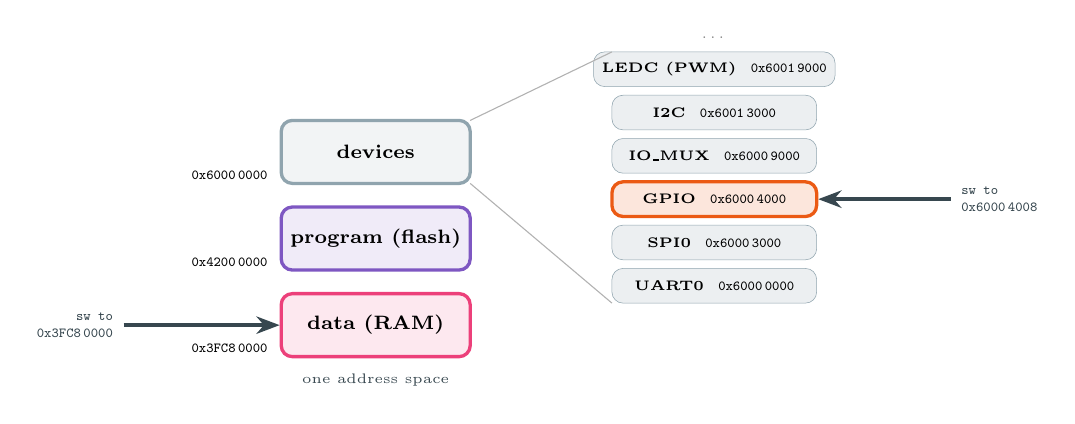
\begin{tikzpicture}[>=Stealth, font=\scriptsize]
    \foreach \y/\n/\a/\c in {2.3/devices/0x6000\,0000/nLine, 1.2/program (flash)/0x4200\,0000/sViolet, 0.1/data (RAM)/0x3FC8\,0000/sPink} {
      \node[lbox, draw=\c, fill=\c!12, minimum width=2.4cm, minimum height=0.8cm] (\n) at (0,\y) {\n};
      \node[font=\ttfamily\tiny, anchor=east] at (-1.25,\y-0.3) {\a};
    }
    \node[font=\tiny, text=nInk, anchor=north] at (0,-0.4) {one address space};
    % the device part, zoomed in: one window per controller
    \foreach \y/\n/\a/\h in {3.35/LEDC (PWM)/0x6001\,9000/0, 2.8/I2C/0x6001\,3000/0, 2.25/IO\_MUX/0x6000\,9000/0,
                             1.7/GPIO/0x6000\,4000/1, 1.15/SPI0/0x6000\,3000/0, 0.6/UART0/0x6000\,0000/0} {
      \ifnum\h=1
        \node[lbox, draw=AccentOrange, fill=AccentOrange!15, minimum width=2.6cm, minimum height=0.44cm, font=\tiny\bfseries] at (4.3,\y) {\n\ \ \texttt{\mdseries\a}};
      \else
        \node[lbox, draw=nLine, fill=nFill, minimum width=2.6cm, minimum height=0.44cm, font=\tiny\bfseries, very thin] at (4.3,\y) {\n\ \ \texttt{\mdseries\a}};
      \fi
    }
    \draw[gray!60, thin] (1.2,2.7) -- (3.0,3.57);
    \draw[gray!60, thin] (1.2,1.9) -- (3.0,0.38);
    \node[font=\tiny, text=gray] at (4.3,3.75) {\ldots};
    % two stores
    \draw[->, very thick, nInk] (7.3,1.7) node[right, font=\tiny\bfseries\ttfamily, align=left] {sw to\\0x6000\,4008} -- (5.62,1.7);
    \draw[->, very thick, nInk] (-3.2,0.1) node[left, font=\tiny\bfseries\ttfamily, align=right] {sw to\\0x3FC8\,0000} -- (-1.22,0.1);
  \end{tikzpicture}}

% ---------- small arrow "program flow" pieces ----------
\tikzset{
  instr/.style={draw=DeepBlue!60, fill=white, minimum width=1.9cm, minimum height=0.38cm, inner sep=1pt,
    font=\ttfamily\tiny},
  isrinstr/.style={instr, draw=cISR, fill=cISR!15},
}

% =====================================================================
%  Day 6 helpers
% =====================================================================

% ---------- names that may still change: Wokwi projects and the simulator ----------
\newcommand{\projCircuit}{\textbf{Circuit}}       % the circuit from Lecture 5
\newcommand{\projLeds}{\textbf{Three LEDs}}       % the circuit with LEDs on GPIO 4, 7 and 3
\newcommand{\projRace}{\textbf{Race}}             % starter code for Task 5
\newcommand{\simname}{\textbf{ComputerHardwareSimulators}}
\newcommand{\simbase}{https://ksawerym.github.io/ComputerHardwareSimulators/}
\newcommand{\simurl}{\href{\simbase}{\texttt{ksawerym.github.io/ComputerHardwareSimulators}}}
% a topic of the simulator: the name links to its section of the page
\expandafter\def\csname simhash@Polling vs interrupt\endcsname{cc-poll}
\expandafter\def\csname simhash@Interrupt step by step\endcsname{cc-irq}
\expandafter\def\csname simhash@Timer and tick\endcsname{cc-tick}
\expandafter\def\csname simhash@Time slice\endcsname{cc-slice}
\expandafter\def\csname simhash@Context switch\endcsname{cc-ctx}
\expandafter\def\csname simhash@States and priorities\endcsname{cc-states}
\expandafter\def\csname simhash@Shared counter\endcsname{cc-shared}
\expandafter\def\csname simhash@Race step by step\endcsname{cc-race}
\expandafter\def\csname simhash@Mutex\endcsname{cc-mutex}
\expandafter\def\csname simhash@Deadlock\endcsname{cc-dead}
\expandafter\def\csname simhash@Producer-consumer\endcsname{cc-pc}
\newcommand{\simhash}[1]{\csname simhash@#1\endcsname}
\newcommand{\simtab}[1]{\href{\simbase\#\simhash{#1}}{\textcolor{DeepBlue}{\textbf{#1}}}}
% the address of a topic, shown at the bottom of a simulator task
\newcommand{\simaddr}[1]{\href{\simbase\#\simhash{#1}}{\texttt{ksawerym.github.io/ComputerHardwareSimulators/\#\simhash{#1}}}}
\newcommand{\simfoot}[1]{\par\vfill{\hfill\scriptsize\textcolor{gray}{\faLink\ #1}\par}}

% ---------- colours used all day ----------
\colorlet{cTaskA}{sViolet}
\colorlet{cTaskB}{sAmber}
\colorlet{cTaskC}{sTeal}
\colorlet{cTaskH}{sBrown}
\colorlet{cSched}{sPink}   % the scheduler runs in the tick interrupt
\colorlet{cLed}{nInk}      % a LED that is on

% ---------- listings ----------
% C++ in Wokwi with the FreeRTOS functions
\lstdefinestyle{rtos}{style=ino,
  morekeywords={TickType_t},
  emph={pinMode,digitalWrite,digitalRead,delay,millis,attachInterrupt,digitalPinToInterrupt,
    timerBegin,timerAttachInterrupt,timerAlarm,xTaskCreate,vTaskDelay,vTaskDelayUntil,vTaskDelete,
    pdMS_TO_TICKS,pcTaskGetName,uxTaskPriorityGet,xTaskGetTickCount}}
% FreeRTOS source code (C)
\lstdefinestyle{frc}{style=cc, morekeywords={StackType_t,ListItem_t,UBaseType_t,TCB_t}}
% RISC-V with the instructions used today
\lstdefinestyle{rv6}{style=rv, morekeywords={j,mret,csrr,csrw}}

% ---------- an interrupt on a timeline ----------
\newcommand{\irqtimeline}{%
  \begin{tikzpicture}[>=Stealth, font=\scriptsize]
    \node[anchor=east, font=\scriptsize\bfseries, text=nInk] at (-0.15,0) {main program};
    \node[anchor=east, font=\scriptsize\bfseries, text=cISR] at (-0.15,-1.0) {ISR};
    \fill[cWork] (0,-0.21) rectangle (3.6,0.21);
    \fill[cWork] (4.8,-0.21) rectangle (9.2,0.21);
    \node[font=\tiny\bfseries, text=white] at (1.8,0) {main program};
    \node[font=\tiny\bfseries, text=white] at (7.0,0) {main program continues};
    \draw[cWork, thick, dashed] (3.6,0) -- (4.8,0);
    \fill[cISR] (3.6,-1.21) rectangle (4.8,-0.79);
    \node[font=\tiny\bfseries, text=white] at (4.2,-1.0) {ISR};
    \draw[->, very thick, DeepBlue] (3.6,-0.25) -- (3.6,-0.75);
    \draw[->, very thick, DeepBlue] (4.8,-0.75) -- (4.8,-0.25);
    \node[anchor=east, font=\scriptsize] at (3.5,-0.5) {\badge{1}\ suspend};
    \node[font=\scriptsize, anchor=north] at (4.2,-1.3) {\badge{2}\ run the ISR};
    \node[anchor=west, font=\scriptsize] at (4.9,-0.5) {\badge{3}\ return};
    % the signal from the button
    \node[font=\Large, text=cIO] at (3.6,1.45) {\faDotCircle};
    \node[anchor=west, font=\scriptsize\bfseries, text=cIO] at (3.95,1.45) {button A is pressed};
    \draw[->, very thick, cIO] (3.6,1.15) -- (3.6,0.3);
    \draw[->, thick, DeepBlue] (0,-1.95) -- (9.4,-1.95) node[right, font=\tiny] {time};
  \end{tikzpicture}}

% ---------- inside the processor: one interrupt in 4 steps ----------
% #1 = step (1 signal, 2 save and jump, 3 the ISR runs, 4 return)
\newcommand{\irqsteps}[1]{%
  \begin{tikzpicture}[>=Stealth, font=\scriptsize,
      hotinstr/.style={instr, fill=AccentOrange!35, draw=AccentOrange, very thick}]
    \useasboundingbox (-1.75,-1.1) rectangle (7.65,2.65);
    % the main program
    \node[font=\scriptsize\bfseries, text=nInk] at (1.6,2.4) {main program};
    \foreach \a/\t [count=\k from 0] in {0x0100/{li\ \ \ t0, 0}, 0x0104/{addi t0, t0, 1},
        0x0108/{sw\ \ \ t0, 0(a0)}, 0x010C/{j\ \ \ \ 0x0104}} {
      \node[addr, font=\ttfamily\tiny, anchor=east] at (0.45,{1.95-0.45*\k}) {\a};
      \node[instr, minimum width=2.2cm] (m\k) at (1.6,{1.95-0.45*\k}) {\t};
    }
    % the ISR
    \node[font=\scriptsize\bfseries, text=cISR] at (5.75,2.4) {ISR: \texttt{onButtonA}};
    \foreach \a/\t [count=\k from 0] in {0x0200/{save t0}, 0x0204/{presses++}, 0x0208/{restore t0},
        0x020C/{return}} {
      \node[addr, font=\ttfamily\tiny, anchor=west] at (6.9,{1.95-0.45*\k}) {\a};
      \node[isrinstr, minimum width=2.2cm] (i\k) at (5.75,{1.95-0.45*\k}) {\t};
    }
    % highlighted instructions
    \ifnum#1=1 \node[hotinstr, minimum width=2.2cm] at (m1) {addi t0, t0, 1}; \fi
    \ifnum#1=3
      \foreach \k in {0,...,3} \draw[cISR, line width=1.6pt] (i\k.south west) rectangle (i\k.north east);
    \fi
    \ifnum#1=4 \node[hotinstr, minimum width=2.2cm] at (m2) {sw\ \ \ t0, 0(a0)}; \fi
    % the signal
    \ifnum#1=1
      \node[font=\scriptsize\bfseries, text=cIO, align=center] (sig) at (-1.05,1.5) {\faDotCircle\\interrupt!};
      \draw[->, very thick, cIO] (sig.east) -- ([xshift=-0.75cm]m1.west);
    \fi
    % jump and return
    \ifnum#1=2 \draw[->, very thick, DeepBlue] (m1.east) to[out=0, in=180] node[pos=0.3, above, font=\tiny\bfseries] {jump} (i0.west); \fi
    \ifnum#1=4 \draw[->, very thick, DeepBlue] (i3.west) to[out=180, in=0] node[pos=0.75, below, font=\tiny\bfseries] {return} (m2.east); \fi
    % registers
    \ifcase#1 \or \def\pcv{0x0104}\def\spcv{--}%
      \or \def\pcv{0x0200}\def\spcv{0x0108}%
      \or \def\pcv{0x0204}\def\spcv{0x0108}%
      \or \def\pcv{0x0108}\def\spcv{0x0108}\fi
    \node[reg, minimum width=2.2cm] (pc) at (1.6,-0.55) {\textbf{PC}\ \ \pcv};
    \node[reg, minimum width=2.2cm, fill=gray!10, draw=gray] (spc) at (5.75,-0.55) {\textbf{saved PC}\ \ \spcv};
    \ifnum#1=2 \draw[WriteRed, line width=1.6pt, rounded corners=2pt] (spc.south west) rectangle (spc.north east); \fi
    \ifnum#1=4
      \draw[ReadBlue, line width=1.6pt, rounded corners=2pt] (spc.south west) rectangle (spc.north east);
      \draw[->, very thick, DeepBlue] (spc.west) -- (pc.east);
    \fi
  \end{tikzpicture}}

% ---------- the button with an interrupt (figure 1 of the course plan) ----------
\newcommand{\figbuttonisr}{%
  \begin{tikzpicture}[>=Stealth, font=\scriptsize]
    \draw[nInk, very thick, rounded corners=6pt, fill=nFill] (0,-0.3) rectangle (4.8,2.75);
    \node[anchor=north west, font=\scriptsize\bfseries, text=nInk] at (0.1,2.7) {\faMicrochip\ ESP32-C3};
    \node[lbox, draw=cISR, fill=cISR!15, minimum width=4.1cm, minimum height=0.85cm] (isr) at (2.4,1.6)
      {interrupt handler (ISR)\\[-1pt]{\ttfamily\mdseries presses++}};
    \node[lbox, draw=cWork, fill=cWork!12, minimum width=4.1cm, minimum height=0.85cm] (main) at (2.4,0.3)
      {main program\\[-1pt]{\mdseries does not check the button}};
    \draw[->, thick, dashed, DeepBlue] (isr.south) -- node[right, font=\tiny] {\texttt{presses}} (main.north);
    \node[lbox, draw=nInk, fill=nFill, minimum width=2.0cm] (btn) at (-2.3,1.6)
      {\faDotCircle\ Button A\\[-1pt]{\tiny\mdseries GPIO 5}};
    \draw[->, very thick, cISR] (btn.east) -- node[above, font=\tiny\bfseries] {interrupt} (isr.west);
    \node[draw=mygreen!60!black, fill=mygreen!55!black, rounded corners=2pt, minimum width=2.5cm,
      minimum height=0.8cm] (lcd) at (7.9,0.3) {};
    \node[fill=LcdScreen!45, minimum width=2.2cm, minimum height=0.5cm, font=\ttfamily\scriptsize] at (lcd) {Presses: 3};
    \node[font=\tiny, anchor=north] at (lcd.south) {LCD 16$\times$2};
    \draw[->, very thick, DeepBlue] (main.east) -- node[pos=0.62, above, font=\tiny] {GPIO 8, 9 (I2C)} (lcd.west);
  \end{tikzpicture}}

% ---------- a timer interrupt every 500 ms ----------
\newcommand{\timertimeline}{%
  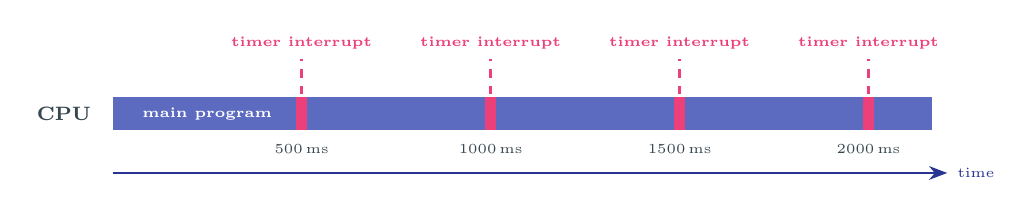
\begin{tikzpicture}[>=Stealth, font=\scriptsize]
    \node[anchor=east, font=\scriptsize\bfseries, text=nInk] at (-0.15,0) {CPU};
    \fill[cWork] (0,-0.21) rectangle (10.4,0.21);
    \node[font=\tiny\bfseries, text=white] at (1.2,0) {main program};
    \foreach \k in {1,...,4} {
      \fill[cISR] ({2.4*\k-0.07},-0.21) rectangle ({2.4*\k+0.07},0.21);
      \draw[cISR, thick, dashed] ({2.4*\k},0.25) -- ({2.4*\k},0.7);
      \node[font=\tiny\bfseries, text=cISR] at ({2.4*\k},0.9) {timer interrupt};
      \node[font=\tiny, text=nInk] at ({2.4*\k},-0.45) {\the\numexpr 500*\k\relax\,ms};
    }
    \draw[->, thick, DeepBlue] (0,-0.75) -- (10.6,-0.75) node[right, font=\tiny] {time};
  \end{tikzpicture}}

% ---------- one tick, three LEDs: #1 = number of ticks ----------
\newcommand{\tickleds}[1]{%
  \begin{tikzpicture}[font=\scriptsize]
    \pgfmathtruncatemacro{\tklast}{#1-1}
    \node[anchor=east, font=\scriptsize\bfseries, text=cISR] at (-0.15,0.55) {tick};
    \foreach \k in {1,...,#1} {
      \draw[cISR, very thick] ({0.42*\k},0.35) -- ({0.42*\k},0.75);
      \node[font=\tiny, text=nInk] at ({0.42*\k},0.95) {\k};
    }
    \foreach \p/\r/\n in {3/1/LED 1, 5/2/LED 2, 7/3/LED 3} {
      \pgfmathsetmacro{\yy}{-0.6*\r+0.3}
      \node[anchor=east, font=\scriptsize\bfseries] at (-0.15,\yy+0.08) {\n};
      \node[anchor=east, font=\tiny, text=gray!40!black] at (-0.15,\yy-0.16) {every \p\ ticks};
      \foreach \k in {0,...,\tklast} {
        \pgfmathtruncatemacro{\s}{mod(floor(\k/\p),2)}
        \ifnum\s=1
          \fill[cLed!75] ({0.42*\k},\yy-0.17) rectangle ({0.42*(\k+1)},\yy+0.17);
        \else
          \fill[gray!12] ({0.42*\k},\yy-0.17) rectangle ({0.42*(\k+1)},\yy+0.17);
        \fi
      }
      \foreach \k in {1,...,#1} {
        \pgfmathtruncatemacro{\rr}{mod(\k,\p)}
        \ifnum\rr=0 \draw[cISR, very thick] ({0.42*\k},\yy-0.24) -- ({0.42*\k},\yy+0.24); \fi
      }
    }
    \draw[decorate, decoration={brace, amplitude=3pt, mirror}, thick, nInk] (0.42,-1.8) -- (0.84,-1.8)
      node[midway, below=3pt, font=\tiny] {100 ms};
    \node[anchor=west, font=\tiny] at (2.0,-1.95) {\textcolor{cLed!75}{\rule{0.25cm}{0.2cm}}\ LED on
      \quad\textcolor{gray!25}{\rule{0.25cm}{0.2cm}}\ LED off
      \quad\textcolor{cISR}{\rule{0.06cm}{0.25cm}}\ the ISR changes the LED};
  \end{tikzpicture}}

% ---------- build it: two more LEDs (GPIO 7 and GPIO 3) ----------
% the circuit of Lecture 5 is faded, the new parts are drawn normally
\newcommand{\buildpicleds}{%
  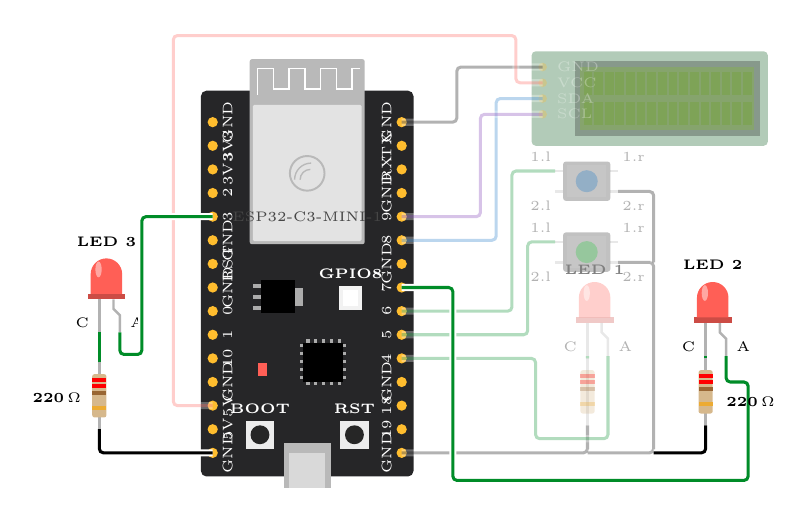
\begin{tikzpicture}[font=\tiny]
    \useasboundingbox (-2.2,-0.25) rectangle (7.3,5.7);
    \pic (esp) at (0,0) {esp32c3};
    \begin{scope}[opacity=0.3]
      % LED 1 and its resistor
      \pic (res) at (4.91,0.65) {wres};
      \pic (led) at (5.0,1.95) {wled};
      \draw[wire, black] (esp-R14) -- (4.91,0.3) -- (res-2);
      \draw[wire, WireGreen] (res-1) -- (led-C);
      \draw[wire, WireGreen] (esp-R10) -| (4.25,0.48) -| (led-A);
      % button A
      \pic (ba) at (4.9,2.85) {wbutton=MacGreen};
      \draw[wire, black] (ba-2r) -| (5.75,0.3) -- (4.91,0.3);
      \draw[wire, WireGreen] (esp-R9) -| ([xshift=-0.35cm]ba-1l) -- (ba-1l);
      % LCD
      \pic (lcd) at (4.2,4.2) {wlcd};
      \draw[wire, black] (esp-R0) -| ([xshift=-1.09cm]lcd-GND) -- (lcd-GND);
      \draw[wire, StorageBlue] (esp-R5) -| ([xshift=-0.59cm]lcd-SDA) -- (lcd-SDA);
      \draw[wire, ProgramPurple] (esp-R4) -| ([xshift=-0.79cm]lcd-SCL) -- (lcd-SCL);
      \draw[wire, MacRed] (esp-L12) -- (-0.35,0.9) -- (-0.35,5.6) -- (4.0,5.6) |- (lcd-VCC);
      % button B
      \pic (bb) at (4.9,3.75) {wbutton=StorageBlue};
      \draw[wire, black] (bb-2r) -| (5.75,2.72);
      \draw[wire, WireGreen] (esp-R8) -| ([xshift=-0.55cm]bb-1l) -- (bb-1l);
    \end{scope}
    \node[font=\fontsize{5.5}{6}\selectfont\bfseries, text=gray] at (5.0,2.62) {LED 1};
    % LED 2 on GPIO 7
    \pic (res2) at (6.41,0.65) {wres};
    \pic (led2) at (6.5,1.95) {wled};
    \draw[wire, black] (res2-2) -- (6.41,0.3) -- (5.75,0.3);
    \draw[wire, WireGreen] (res2-1) -- (led2-C);
    \draw[wire, WireGreen] (esp-R7) -- (3.2,2.4) -- (3.2,-0.05) -- (6.95,-0.05) -- (6.95,1.2) -- (6.67,1.2) -- (led2-A);
    \node[font=\fontsize{5.5}{6}\selectfont\bfseries, anchor=south] at (6.5,2.5) {LED 2};
    % LED 3 on GPIO 3
    \pic (res3) at (-1.29,0.6) {wres};
    \pic (led3) at (-1.2,2.25) {wled};
    \draw[wire, black] (res3-2) -- (-1.29,0.3) -- (esp-L14);
    \draw[wire, WireGreen] (res3-1) -- (led3-C);
    \draw[wire, WireGreen] (esp-L4) -- (-0.75,3.3) -- (-0.75,1.55) -- (-1.03,1.55) -- (led3-A);
    \node[font=\fontsize{5.5}{6}\selectfont\bfseries, anchor=south] at (-1.2,2.8) {LED 3};
    \node[font=\fontsize{5.5}{6}\selectfont\bfseries, anchor=east] at (-1.4,1.0) {220\,$\Omega$};
    \node[font=\fontsize{5.5}{6}\selectfont\bfseries, anchor=west] at (6.55,0.95) {220\,$\Omega$};
  \end{tikzpicture}}

% ---------- three LEDs, a button and the LCD (figure 2 of the course plan) ----------
\newcommand{\figthreeleds}{%
  \begin{tikzpicture}[>=Stealth, font=\scriptsize]
    \draw[nInk, very thick, rounded corners=6pt, fill=nFill] (0,-0.35) rectangle (4.0,3.75);
    \node[anchor=north west, font=\scriptsize\bfseries, text=nInk] at (0.1,3.7) {\faMicrochip\ ESP32-C3};
    \node[lbox, draw=cISR, fill=cISR!15, minimum width=3.5cm, minimum height=0.8cm] (tisr) at (2.0,2.6)
      {Timer ISR\\[-1pt]{\mdseries every 100 ms: 3 LEDs}};
    \node[lbox, draw=cISR, fill=cISR!15, minimum width=3.5cm, minimum height=0.8cm] (bisr) at (2.0,1.5)
      {Button ISR\\[-1pt]{\ttfamily\mdseries presses++}};
    \node[lbox, draw=cWork, fill=cWork!12, minimum width=3.5cm, minimum height=0.8cm] (main) at (2.0,0.4)
      {main loop\\[-1pt]{\mdseries counts}};
    \foreach \y/\g/\n in {3.3/4/1, 2.6/7/2, 1.9/3/3} {
      \draw[->, thick, cISR] (tisr.east) -- (5.35,\y);
      \fill[cLed] (5.55,\y) circle (0.15);
      \node[anchor=west, font=\scriptsize] at (5.8,\y) {LED \n\ (GPIO \g)};
    }
    \node[lbox, draw=nInk, fill=nFill, minimum width=1.9cm] (btn) at (-1.9,1.5)
      {\faDotCircle\ Button A\\[-1pt]{\mdseries GPIO 5}};
    \draw[->, very thick, cISR] (btn.east) -- (bisr.west);
    \node[draw=mygreen!60!black, fill=mygreen!55!black, rounded corners=2pt, minimum width=2.6cm,
      minimum height=1.05cm] (lcd) at (6.4,0.4) {};
    \node[fill=LcdScreen!45, minimum width=2.3cm, minimum height=0.8cm, font=\ttfamily\scriptsize, align=left] at (lcd)
      {Presses: 3\\Loop: 18452};
    \draw[->, very thick, DeepBlue] (main.east) -- (lcd.west);
  \end{tikzpicture}}

% ---------- three ways to keep a rhythm: #1 = 1 delay(), 2 millis() in loop(), 3 timer interrupt ----------
\newcommand{\rhythm}[1]{%
  \begin{tikzpicture}[>=Stealth, font=\tiny]
    \useasboundingbox (-0.1,-1.0) rectangle (4.6,0.95);
    \ifnum#1=1
      \node[draw=white, fill=cIdle, minimum width=0.9cm, minimum height=0.42cm, inner sep=0pt, anchor=west,
        font=\tiny\bfseries, text=white] at (0,0) {LED 1};
      \node[draw=white, fill=cIdle, minimum width=1.5cm, minimum height=0.42cm, inner sep=0pt, anchor=west,
        font=\tiny\bfseries, text=white] at (0.9,0) {wait for LED 2};
      \node[draw=white, fill=cIdle, minimum width=2.1cm, minimum height=0.42cm, inner sep=0pt, anchor=west,
        font=\tiny\bfseries, text=white] at (2.4,0) {wait for LED 3};
      \node[font=\tiny\bfseries, text=nInk, anchor=south] at (2.25,0.3) {\texttt{delay}: 300 + 500 + 700 ms, one after another};
      \draw[<->, thick, AccentOrange] (0,-0.45) -- node[below, font=\tiny\bfseries] {LED 1 changes again only after 1.5 s} (4.5,-0.45);
    \else
      \fill[cWork] (0,-0.21) rectangle (4.5,0.21);
      \foreach \a in {0.5,1.6,2.6,3.5} {
        \fill[cIdle] (\a,-0.21) rectangle (\a+0.6,0.21);
        \node[font=\tiny\bfseries, text=white] at (\a+0.3,0) {LCD};
      }
      \foreach \x in {0.9,1.8,2.7,3.6} \draw[nInk, dashed, thick] (\x,0.25) -- (\x,0.6);
      \node[font=\tiny, text=nInk, anchor=south] at (2.25,0.6) {when LED 1 should change};
    \fi
    \ifnum#1=2
      \foreach \x/\y in {0.9/1.1, 1.8/2.2, 2.7/3.2, 3.6/4.1} {
        \draw[AccentOrange, very thick] (\y,-0.28) -- (\y,-0.55);
        \draw[->, nInk, thick] (\x,-0.42) -- (\y-0.03,-0.42);
      }
      \node[font=\tiny\bfseries, text=AccentOrange, anchor=north] at (2.25,-0.6) {LED 1 changes late: after each LCD write};
    \fi
    \ifnum#1=3
      \foreach \x in {0.9,1.8,2.7,3.6} {
        \fill[cISR] (\x-0.04,-0.21) rectangle (\x+0.04,0.21);
        \draw[cISR, very thick] (\x,-0.28) -- (\x,-0.55);
      }
      \node[font=\tiny\bfseries, text=cISR, anchor=north] at (2.25,-0.6) {LED 1 changes on time, even during the LCD write};
    \fi
  \end{tikzpicture}}

% ---------- one core, three tasks ----------
\newcommand{\oneprocessor}{%
  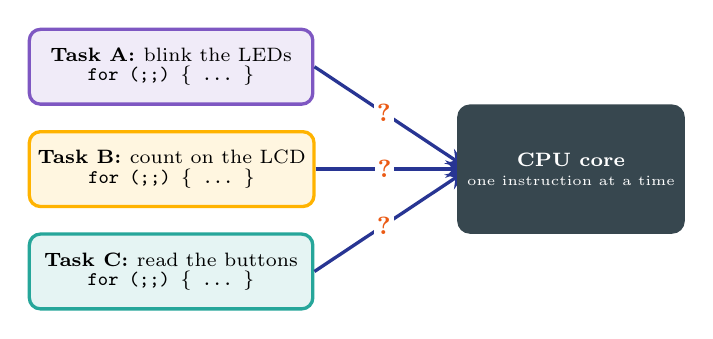
\begin{tikzpicture}[>=Stealth, font=\scriptsize]
    \foreach \n/\c/\w/\y in {A/cTaskA/blink the LEDs/1.3, B/cTaskB/count on the LCD/0, C/cTaskC/read the buttons/-1.3} {
      \node[lbox, draw=\c, fill=\c!12, minimum width=3.6cm, minimum height=0.95cm, anchor=west] (t\n) at (0,\y)
        {Task \n: {\mdseries \w}\\[-1pt]{\ttfamily\mdseries for (;;) \{ \ldots\ \}}};
      \draw[->, very thick, DeepBlue] (t\n.east) -- (5.6,0) node[pos=0.45, fill=white, font=\small\bfseries,
        text=AccentOrange, inner sep=1pt] {?};
    }
    \node[cpubox, minimum width=2.6cm, minimum height=1.6cm] at (6.9,0)
      {CPU core\\[-1pt]{\tiny\mdseries one instruction at a time}};
  \end{tikzpicture}}

% ---------- time slices, and how it looks to us ----------
\newcommand{\timeslices}{%
  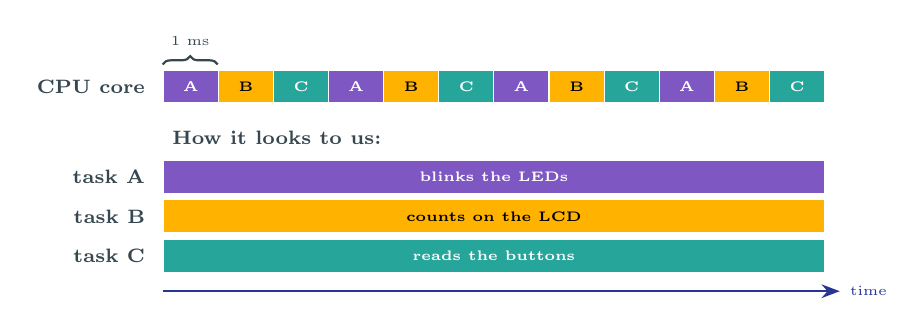
\begin{tikzpicture}[>=Stealth, font=\scriptsize]
    \tlbar{0}{CPU core}{0.7/cTaskA/A,0.7/cTaskB/B,0.7/cTaskC/C,0.7/cTaskA/A,0.7/cTaskB/B,0.7/cTaskC/C,
      0.7/cTaskA/A,0.7/cTaskB/B,0.7/cTaskC/C,0.7/cTaskA/A,0.7/cTaskB/B,0.7/cTaskC/C}
    \draw[decorate, decoration={brace, amplitude=3pt}, thick, nInk] (0,0.28) -- (0.7,0.28)
      node[midway, above=3pt, font=\tiny] {1 ms};
    \node[anchor=west, font=\scriptsize\bfseries, text=nInk] at (0,-0.65) {How it looks to us:};
    \tlbar{-1.15}{task A}{8.4/cTaskA/blinks the LEDs}
    \tlbar{-1.65}{task B}{8.4/cTaskB/counts on the LCD}
    \tlbar{-2.15}{task C}{8.4/cTaskC/reads the buttons}
    \draw[->, thick, DeepBlue] (0,-2.6) -- (8.6,-2.6) node[right, font=\tiny] {time};
  \end{tikzpicture}}

% ---------- the tick wakes the scheduler ----------
\newcommand{\tickscheduler}{%
  \begin{tikzpicture}[>=Stealth, font=\scriptsize]
    \node[lbox, draw=cISR, fill=cISR!15, minimum width=1.8cm, minimum height=0.9cm] (tim) at (0,0) {\faClock\ timer};
    \node[lbox, draw=cSched, fill=cSched!20, minimum width=2.3cm, minimum height=0.9cm] (sch) at (3.7,0)
      {scheduler\\[-1pt]{\tiny\mdseries which task next?}};
    \draw[->, very thick, cISR] (tim) -- node[above, font=\tiny\bfseries] {tick} node[below, font=\tiny] {every 1 ms} (sch);
    \node[lbox, draw=cTaskA, fill=cTaskA!12, minimum width=1.5cm] (a) at (7.0,1.0) {Task A};
    \node[lbox, draw=cTaskB, fill=cTaskB!25, minimum width=1.5cm, line width=2pt] (b) at (7.0,0) {Task B};
    \node[lbox, draw=cTaskC, fill=cTaskC!12, minimum width=1.5cm] (c) at (7.0,-1.0) {Task C};
    \draw[->, thick, DeepBlue!50] (sch.east) -- (a.west);
    \draw[->, line width=2pt, DeepBlue] (sch.east) -- (b.west);
    \draw[->, thick, DeepBlue!50] (sch.east) -- (c.west);
    \node[anchor=west, font=\tiny\bfseries, text=sAmberText] at (7.85,0) {runs now};
  \end{tikzpicture}}

% ---------- each task has its own stack ----------
\newcommand{\stackmem}{%
  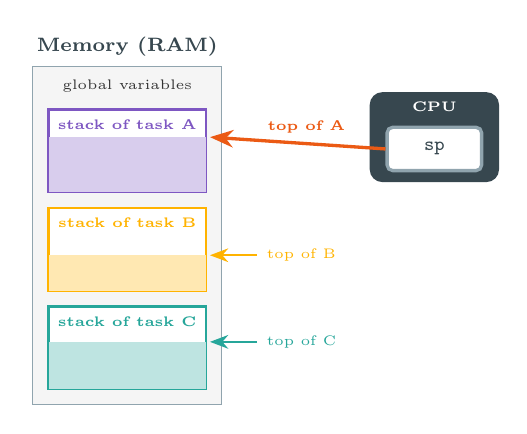
\begin{tikzpicture}[>=Stealth, font=\scriptsize]
    \node[font=\scriptsize\bfseries, text=nInk] at (1.2,4.55) {Memory (RAM)};
    \draw[nLine, fill=gray!8] (0,0) rectangle (2.4,4.3);
    \node[font=\tiny, text=gray!40!black] at (1.2,4.05) {global variables};
    \foreach \n/\c/\yb/\h in {A/cTaskA/2.7/0.7, B/cTaskB/1.45/0.45, C/cTaskC/0.2/0.6} {
      \draw[\c, thick, fill=white] (0.2,\yb) rectangle (2.2,\yb+1.05);
      \fill[\c!30] (0.2,\yb) rectangle (2.2,\yb+\h);
      \node[font=\tiny\bfseries, text=\c] at (1.2,\yb+0.86) {stack of task \n};
    }
    \foreach \n/\c/\t in {B/cTaskB/1.9, C/cTaskC/0.8} {
      \draw[->, thick, \c] (2.85,\t) -- (2.25,\t);
      \node[anchor=west, font=\tiny, text=\c] at (2.85,\t) {top of \n};
    }
    \node[cpubox, minimum width=1.6cm, minimum height=1.1cm] (cpu) at (5.1,3.4) {};
    \node[font=\tiny\bfseries, text=white, anchor=north] at (cpu.north) {CPU};
    \node[reg, minimum width=1.2cm] (sp) at (5.1,3.25) {\textbf{sp}};
    \draw[->, very thick, AccentOrange] (sp.west) -- (2.25,3.4) node[pos=0.45, above, font=\tiny\bfseries] {top of A};
  \end{tikzpicture}}

% ---------- context switch in 4 steps ----------
% #1 = step (1 tick, 2 save A, 3 choose B, 4 restore B)
\newcommand{\ctxswitch}[1]{%
  \begin{tikzpicture}[>=Stealth, font=\scriptsize,
      cell/.style={draw=nLine, minimum width=1.8cm, minimum height=0.42cm, inner sep=0pt, font=\ttfamily\tiny},
      src/.style={aread},
      dst/.style={awrite},
      tcell/.style={draw=nLine, fill=white, minimum height=0.45cm, inner sep=0pt}]
    \useasboundingbox (-0.2,-0.7) rectangle (12.5,4.75);
    % ----- the CPU -----
    \draw[nInk, very thick, rounded corners=6pt, fill=nFill] (0,0) rectangle (3.0,3.6);
    \node[anchor=north west, font=\scriptsize\bfseries, text=nInk] at (0.08,3.55) {CPU};
    \ifcase#1 \or \def\running{task A}\or \def\running{scheduler}\or \def\running{scheduler}\or \def\running{task B}\fi
    \node[anchor=north east, font=\tiny] at (2.95,3.55) {running: \textbf{\running}};
    \ifnum#1<4 \colorlet{ctxc}{cTaskA}\def\who{A}\else \colorlet{ctxc}{cTaskB}\def\who{B}\fi
    \foreach \r/\y in {PC/2.75, t0/2.1, t1/1.45} {
      \node[draw=ctxc, very thick, fill=ctxc!12, rounded corners=2pt, minimum width=2.4cm, minimum height=0.48cm,
        font=\ttfamily\scriptsize] at (1.5,\y) {\textbf{\r}\ \ \who's \r};
    }
    \node[draw=ctxc, very thick, fill=ctxc!12, rounded corners=2pt, minimum width=2.4cm, minimum height=0.48cm,
      font=\ttfamily\scriptsize] at (1.5,0.55) {\textbf{sp}\ \ top of \who};
    \ifnum#1=2
      \draw[src, rounded corners=3pt] (0.22,1.14) rectangle (2.78,3.06);
      \draw[src, rounded corners=3pt] (0.22,0.24) rectangle (2.78,0.86);
    \fi
    \ifnum#1=4
      \draw[dst, rounded corners=3pt] (0.22,1.14) rectangle (2.78,3.06);
      \draw[dst, rounded corners=3pt] (0.22,0.24) rectangle (2.78,0.86);
    \fi
    % ----- the two stacks -----
    \foreach \sx/\n/\c in {4.9/A/cTaskA, 7.6/B/cTaskB} {
      \node[font=\scriptsize\bfseries, text=\c] at (\sx,3.3) {stack of \n};
      \draw[\c, thick] (\sx-0.95,0.15) rectangle (\sx+0.95,3.0);
      \node[cell, fill=\c!8, font=\tiny] at (\sx,0.45) {data of \n};
      \node[cell, fill=\c!8, font=\tiny] at (\sx,0.87) {data of \n};
    }
    \ifnum#1>1
      \foreach \r/\y in {t1/1.29, t0/1.71, PC/2.13} \node[cell, fill=cTaskA!30] at (4.9,\y) {A's \r};
    \else
      \foreach \y in {1.29,1.71,2.13} \node[cell, draw=nLight, dashed] at (4.9,\y) {};
    \fi
    \ifnum#1=2 \draw[dst, rounded corners=2pt] (3.98,1.06) rectangle (5.82,2.36); \fi
    \foreach \r/\y in {t1/1.29, t0/1.71, PC/2.13} \node[cell, fill=cTaskB!30] at (7.6,\y) {B's \r};
    \ifnum#1=4 \draw[src, rounded corners=2pt] (6.68,1.06) rectangle (8.52,2.36); \fi
    % top of each stack
    \ifnum#1>1 \def\topA{2.34}\else \def\topA{1.08}\fi
    \ifnum#1>3 \def\topB{1.08}\else \def\topB{2.34}\fi
    \draw[->, thick, cTaskA] (6.15,\topA) -- (5.88,\topA);
    \node[anchor=west, font=\tiny, text=cTaskA] at (6.12,\topA) {top};
    \draw[->, thick, cTaskB] (8.85,\topB) -- (8.58,\topB);
    \node[anchor=west, font=\tiny, text=sAmberText] at (8.82,\topB) {top};
    % ----- the table of saved stack pointers -----
    \node[draw=nInk, fill=nInk, text=white, font=\tiny\bfseries, minimum width=2.6cm, minimum height=0.42cm]
      at (10.7,3.0) {saved sp};
    \ifnum#1>1 \def\valA{top of A}\else \def\valA{--}\fi
    \node[tcell, minimum width=0.9cm, font=\tiny\bfseries, text=cTaskA] at (9.85,2.55) {task A};
    \node[tcell, minimum width=1.7cm, font=\ttfamily\tiny] (va) at (11.15,2.55) {\valA};
    \node[tcell, minimum width=0.9cm, font=\tiny\bfseries, text=sAmberText] at (9.85,2.1) {task B};
    \node[tcell, minimum width=1.7cm, font=\ttfamily\tiny] (vb) at (11.15,2.1) {top of B};
    \ifnum#1=2 \draw[dst] (va.south west) rectangle (va.north east); \fi
    \ifnum#1=3 \draw[cSched, line width=1.6pt] (9.4,1.875) rectangle (12.0,2.325); \fi
    \ifnum#1=4 \draw[src] (vb.south west) rectangle (vb.north east); \fi
    % ----- legend -----
    \node[font=\tiny, anchor=west] at (4.1,4.4) {\tikz[baseline=-0.6ex]\draw[aread] (0,-0.07) rectangle (0.32,0.11);\ read from here
      \quad\tikz[baseline=-0.6ex]\draw[awrite] (0,-0.07) rectangle (0.32,0.11);\ written here
      \quad\textcolor{cTaskA}{\rule{0.25cm}{0.2cm}}\ task A
      \quad\textcolor{cTaskB}{\rule{0.25cm}{0.2cm}}\ task B};
    % ----- what happens in this step -----
    \ifnum#1=1
      \node[lbox, draw=cISR, fill=cISR!15] (tick) at (1.5,4.3) {\faClock\ tick: timer interrupt};
      \draw[->, very thick, cISR] (tick) -- (1.5,3.62);
    \fi
    \ifnum#1=2
      \draw[->, very thick, DeepBlue] (2.8,2.1) -- (3.96,1.71);
      \draw[->, very thick, DeepBlue, rounded corners=3pt] (2.8,0.55) -- (3.4,0.55) -- (3.4,-0.45) -- (12.3,-0.45)
        -- (12.3,2.55) -- (12.02,2.55);
    \fi
    \ifnum#1=3
      \node[lbox, draw=cSched, fill=cSched!20] (sch) at (10.7,1.1) {scheduler: next task = B};
      \draw[->, very thick, cSched] (sch) -- (10.7,1.86);
    \fi
    \ifnum#1=4
      \draw[->, very thick, DeepBlue, rounded corners=3pt] (12.02,2.1) -- (12.3,2.1) -- (12.3,-0.45) -- (3.4,-0.45)
        -- (3.4,0.55) -- (2.82,0.55);
      \draw[->, very thick, DeepBlue, rounded corners=3pt] (8.54,1.71) -- (9.0,1.71) -- (9.0,3.75) -- (3.3,3.75)
        -- (3.3,2.1) -- (2.82,2.1);
    \fi
  \end{tikzpicture}}
\newcommand{\ctxlegend}{%
  {\tiny\tikz[baseline=-0.6ex]\draw[aread] (0,-0.07) rectangle (0.32,0.11);\ read from here
  \qquad\tikz[baseline=-0.6ex]\draw[awrite] (0,-0.07) rectangle (0.32,0.11);\ written here
  \qquad\textcolor{cTaskA}{\rule{0.25cm}{0.2cm}}\ task A
  \qquad\textcolor{cTaskB}{\rule{0.25cm}{0.2cm}}\ task B}}

% ---------- task states ----------
\newcommand{\taskstates}{%
  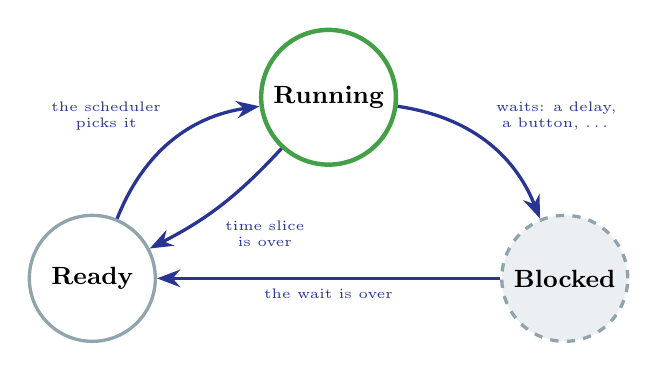
\begin{tikzpicture}[>=Stealth, font=\scriptsize,
      st/.style={circle, very thick, minimum size=1.6cm, font=\small\bfseries, align=center}]
    \node[st, aexec, fill=white] (run) at (0,2.3) {Running};
    \node[st, draw=nLine, fill=white] (rdy) at (-3.0,0) {Ready};
    \node[st, draw=nLine, dashed, fill=nFill] (blk) at (3.0,0) {Blocked};
    \draw[->, very thick, DeepBlue] (rdy) to[bend left=30] node[above left, font=\tiny, align=center] {the scheduler\\picks it} (run);
    \draw[->, very thick, DeepBlue] (run) to[bend left=10] node[below right, font=\tiny, align=center, pos=0.55] {time slice\\is over} (rdy);
    \draw[->, very thick, DeepBlue] (run) to[bend left=30] node[above right, font=\tiny, align=center] {waits: a delay,\\a button, \ldots} (blk);
    \draw[->, very thick, DeepBlue] (blk) -- node[below, font=\tiny] {the wait is over} (rdy);
  \end{tikzpicture}}

% ---------- round robin and priorities ----------
\newcommand{\rrqueue}{%
  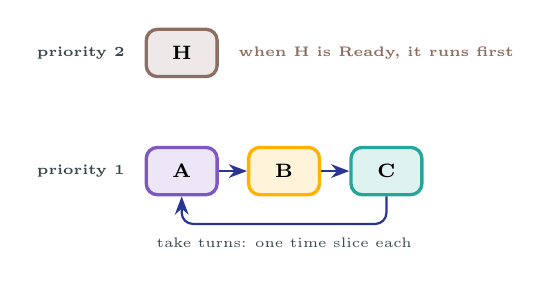
\begin{tikzpicture}[>=Stealth, font=\scriptsize, tk/.style={lbox, minimum width=0.9cm, minimum height=0.6cm}]
    \node[font=\tiny\bfseries, text=nInk, anchor=east] at (-0.6,1.5) {priority 2};
    \node[tk, draw=cTaskH, fill=cTaskH!15] (h) at (0,1.5) {H};
    \node[anchor=west, font=\tiny\bfseries, text=cTaskH] at (0.6,1.5) {when H is Ready, it runs first};
    \node[font=\tiny\bfseries, text=nInk, anchor=east] at (-0.6,0) {priority 1};
    \node[tk, draw=cTaskA, fill=cTaskA!15] (a) at (0,0) {A};
    \node[tk, draw=cTaskB, fill=cTaskB!15] (b) at (1.3,0) {B};
    \node[tk, draw=cTaskC, fill=cTaskC!15] (c) at (2.6,0) {C};
    \draw[->, thick, DeepBlue] (a) -- (b);
    \draw[->, thick, DeepBlue] (b) -- (c);
    \draw[->, thick, DeepBlue, rounded corners=4pt] (c.south) -- ++(0,-0.35) -| (a.south);
    \node[font=\tiny, text=nInk, anchor=north] at (1.3,-0.72) {take turns: one time slice each};
  \end{tikzpicture}}

% ---------- FreeRTOS on our ESP32-C3 ----------
\newcommand{\rtostasks}{%
  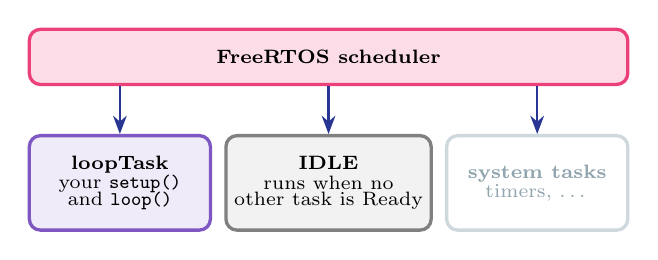
\begin{tikzpicture}[>=Stealth, font=\scriptsize]
    \node[lbox, draw=cSched, fill=cSched!18, minimum width=7.6cm, minimum height=0.7cm] (s) at (0,1.6) {FreeRTOS scheduler};
    \node[lbox, draw=cTaskA, fill=cTaskA!12, minimum width=2.3cm, minimum height=1.2cm] (l) at (-2.65,0)
      {loopTask\\[-1pt]{\mdseries your \texttt{setup()}}\\[-2pt]{\mdseries and \texttt{loop()}}};
    \node[lbox, draw=gray, fill=gray!10, minimum width=2.3cm, minimum height=1.2cm] (i) at (0,0)
      {IDLE\\[-1pt]{\mdseries runs when no}\\[-2pt]{\mdseries other task is Ready}};
    \node[greybox, minimum width=2.3cm, minimum height=1.2cm] (y) at (2.65,0)
      {system tasks\\[-1pt]{\mdseries timers, \ldots}};
    \foreach \t in {l,i,y} \draw[->, thick, DeepBlue] (s.south -| \t) -- (\t.north);
  \end{tikzpicture}}

% ---------- the Ready lists of FreeRTOS ----------
\newcommand{\readylists}{%
  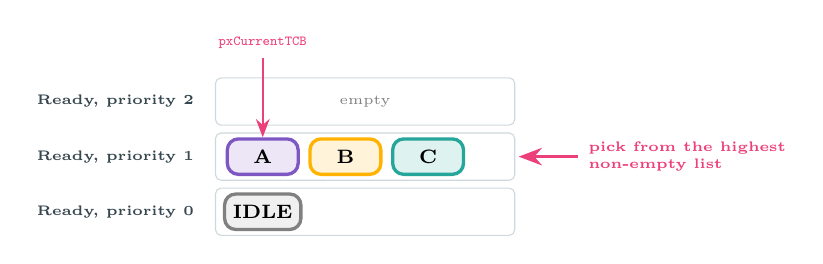
\begin{tikzpicture}[>=Stealth, font=\scriptsize, tk/.style={lbox, minimum width=0.9cm, minimum height=0.45cm}]
    \foreach \p/\y in {2/1.0, 1/0.3, 0/-0.4} {
      \node[font=\tiny\bfseries, text=nInk, anchor=east] at (-0.15,\y) {Ready, priority \p};
      \draw[nLight, rounded corners=2pt] (0,\y-0.3) rectangle (3.8,\y+0.3);
    }
    \node[font=\tiny, text=gray] at (1.9,1.0) {empty};
    \node[tk, draw=cTaskA, fill=cTaskA!15] (a) at (0.6,0.3) {A};
    \node[tk, draw=cTaskB, fill=cTaskB!15] at (1.65,0.3) {B};
    \node[tk, draw=cTaskC, fill=cTaskC!15] at (2.7,0.3) {C};
    \node[tk, draw=gray, fill=gray!12] at (0.6,-0.4) {IDLE};
    \draw[<-, very thick, cSched] (3.85,0.3) -- (4.6,0.3) node[right, font=\tiny\bfseries, align=left]
      {pick from the highest\\non-empty list};
    \node[font=\tiny\ttfamily, text=cSched, anchor=south] (cur) at (0.6,1.55) {pxCurrentTCB};
    \draw[->, thick, cSched] (cur.south) to[out=-90, in=90] (a.north);
  \end{tikzpicture}}

% ---------- two tasks, one counter ----------
\newcommand{\racetimeline}{%
  \begin{tikzpicture}[>=Stealth, font=\scriptsize]
    \node[anchor=east, font=\scriptsize\bfseries, text=cTaskA] at (-0.15,0.5) {Task A};
    \node[anchor=east, font=\scriptsize\bfseries, text=sAmberText] at (-0.15,0) {Task B};
    \foreach \k in {0,...,6} {
      \fill[cTaskA] ({1.2*\k},0.29) rectangle ({1.2*\k+0.6},0.71);
      \fill[cTaskB] ({1.2*\k+0.6},-0.21) rectangle ({1.2*\k+1.2},0.21);
    }
    \node[font=\tiny\bfseries, text=white] at (0.3,0.5) {\texttt{++}};
    \node[font=\tiny\bfseries, text=black] at (0.9,0) {\texttt{++}};
    \draw[AccentOrange, very thick, dashed] (3.0,-0.4) -- (3.0,1.1);
    \node[font=\large, text=AccentOrange] at (3.0,1.35) {\faBolt};
    \node[font=\tiny\bfseries, text=AccentOrange, anchor=west] at (3.25,1.35) {a switch at a bad moment: some updates are lost};
    \draw[->, thick, DeepBlue] (0,-0.55) -- (8.6,-0.55) node[right, font=\tiny] {time};
    \node[font=\tiny, anchor=north] at (4.2,-0.65) {one time slice = 1 ms: thousands of \texttt{counter++} each};
  \end{tikzpicture}}

% ---------- only one task at a time may update the counter ----------
\newcommand{\lockbox}{%
  \begin{tikzpicture}[>=Stealth, font=\scriptsize]
    \node[draw=AccentOrange, very thick, rounded corners=4pt, fill=AccentOrange!10, minimum width=3.8cm,
      minimum height=1.4cm, align=center] (cs) at (0,0)
      {{\Large\textcolor{AccentOrange}{\faLock}}\\[3pt]\texttt{counter++;}};
    \node[font=\tiny\bfseries, text=AccentOrange, anchor=north] at ([yshift=-2pt]cs.south) {must not be interrupted by the other task};
    \node[lbox, draw=cTaskA, fill=cTaskA!12, minimum width=1.6cm] (a) at (-4.2,0.45) {Task A};
    \node[lbox, draw=cTaskB, fill=cTaskB!12, minimum width=1.6cm] (b) at (-4.2,-0.45) {Task B};
    \draw[->, very thick, cTaskA] (a.east) -- (cs.west |- a.east) node[pos=0.5, above, font=\tiny] {inside};
    \draw[->, very thick, cTaskB] (b.east) -- (-2.45,-0.45);
    \node[font=\tiny, text=sAmberText, anchor=north] at (-2.75,-0.6) {\faHourglassHalf\ waits};
  \end{tikzpicture}}


% =====================================================================
%  Day 7 helpers
% =====================================================================

% ---------- the names of the starter files (on GitHub) ----------
\newcommand{\fileRace}{\texttt{race.cpp}}
\newcommand{\fileBank}{\texttt{bank.cpp}}

% ---------- colours used all day ----------
% threads use the task colours of Day 6: cTaskA, cTaskB, cTaskC, cTaskH
\colorlet{cLock}{nFill}    % lock / unlock: neutral, with the word inside
\colorlet{cWait}{nIdle}
\colorlet{cShared}{nLine}  % the shared counter, the accounts: data

% ---------- listings ----------
% C++ on the laptop (@...@ = part to change, shown in yellow)
\lstdefinestyle{cpp}{language=C++, basicstyle=\color{VSText}\ttfamily\scriptsize, numbers=none,
  keywordstyle=\color{VSBlue}\bfseries, commentstyle=\color{VSComment}\itshape, stringstyle=\color{VSString},
  columns=fixed, basewidth=0.52em, keepspaces=true, breaklines=false, showstringspaces=false, xleftmargin=6pt,
  morekeywords={std,thread,mutex,lock_guard,scoped_lock,atomic,vector,mt19937,uniform_int_distribution,
    chrono,steady_clock,duration,milli},
  emph={join,emplace_back,hardware_concurrency,now,count,ref,lock,unlock},
  emphstyle=\color{VSPurple},
  deletestring=[b]{'},
  moredelim=[is][\color{MacYellow}\bfseries]{@}{@}}
% RISC-V with the atomic instructions
\lstdefinestyle{rv7}{style=rv, morekeywords={lui,amoadd.w,lr.w,sc.w}}

% ---------- one core takes turns, four cores work at the same moment ----------
\newcommand{\concpar}{%
  \begin{tikzpicture}[>=Stealth, font=\scriptsize]
    % one core
    \node[font=\scriptsize\bfseries, text=nInk, anchor=west] at (-0.8,1.15) {\faMicrochip\ ESP32-C3: 1 core};
    \tlbar{-0.15}{core}{0.5/cTaskA/A,0.5/cTaskB/B,0.5/cTaskC/C,0.5/cTaskH/D,0.5/cTaskA/A,0.5/cTaskB/B,0.5/cTaskC/C,0.5/cTaskH/D}
    \draw[->, thick, DeepBlue] (0,-1.3) -- (4.2,-1.3) node[right, font=\tiny] {time};
    \node[font=\scriptsize\bfseries, text=AccentOrange] at (2.0,-1.75) {concurrency: taking turns};
    % four cores
    \begin{scope}[xshift=7.0cm]
      \node[font=\scriptsize\bfseries, text=nInk, anchor=west] at (-1.0,1.15) {\faLaptop\ laptop: 4 cores};
      \tlbar{0.6}{core 1}{4.0/cTaskA/A}
      \tlbar{0.1}{core 2}{4.0/cTaskB/B}
      \tlbar{-0.4}{core 3}{4.0/cTaskC/C}
      \tlbar{-0.9}{core 4}{4.0/cTaskH/D}
      \draw[->, thick, DeepBlue] (0,-1.3) -- (4.2,-1.3) node[right, font=\tiny] {time};
      \node[font=\scriptsize\bfseries, text=AccentOrange] at (2.0,-1.75) {parallelism: at the same moment};
    \end{scope}
  \end{tikzpicture}}

% ---------- a processor with 4 cores (as in Lecture 4) ----------
\newcommand{\multicore}{%
  \begin{tikzpicture}[>=Stealth, font=\scriptsize]
    \draw[nInk, very thick, rounded corners=6pt, fill=nFill] (-1.0,-0.6) rectangle (6.4,2.65);
    \node[anchor=north west, font=\scriptsize\bfseries, text=nInk] at (-0.95,2.6) {processor};
    \foreach \i in {1,...,4} {
      \pgfmathsetmacro{\xx}{1.8*(\i-1)}
      \node[cpubox, minimum width=1.5cm, minimum height=0.55cm] at (\xx,1.7) {core \i};
      \node[cachebox, minimum width=1.5cm, minimum height=0.32cm, font=\tiny\bfseries, inner sep=1pt] at (\xx,1.15) {L1};
      \node[cachebox, minimum width=1.5cm, minimum height=0.32cm, font=\tiny\bfseries, inner sep=1pt] at (\xx,0.72) {L2};
    }
    \node[cachebox, minimum width=6.9cm, minimum height=0.4cm] at (2.7,0.1) {L3: shared by all cores};
    \node[rambox, minimum width=6.9cm, minimum height=0.45cm] at (2.7,-1.15) {RAM: \texttt{counter} lives here};
    \draw[<->, very thick, DeepBlue] (2.7,-0.6) -- (2.7,-0.9);
  \end{tikzpicture}}

% ---------- processes and threads ----------
\newcommand{\procthreads}{%
  \begin{tikzpicture}[>=Stealth, font=\scriptsize]
    % process 1
    \draw[nInk, very thick, rounded corners=6pt, fill=nFill] (0,0) rectangle (7.2,3.6);
    \node[anchor=north west, font=\scriptsize\bfseries, text=nInk] at (0.1,3.55) {process 1: our program};
    \node[lbox, draw=nLine, fill=nFill, text=nInk, minimum width=6.6cm, minimum height=0.75cm] (sh) at (3.6,2.55)
      {shared memory\\[-1pt]{\mdseries code, global variables (\texttt{counter}), heap}};
    \foreach \i/\c/\x in {1/cTaskA/1.2, 2/cTaskB/3.6, 3/cTaskC/6.0} {
      \node[lbox, draw=\c, fill=\c!12, minimum width=2.1cm, minimum height=1.05cm] (t\i) at (\x,0.75)
        {thread \i\\[-1pt]{\mdseries own stack}\\[-2pt]{\mdseries own registers}};
      \draw[<->, very thick, \c] (t\i.north) -- (t\i.north |- sh.south);
    }
    % process 2
    \draw[nLight, very thick, rounded corners=6pt, fill=white] (7.8,0) rectangle (10.4,3.6);
    \node[anchor=north west, font=\scriptsize\bfseries, text=gray!40!black] at (7.9,3.55) {process 2};
    \node[greybox, minimum width=2.1cm, minimum height=0.75cm] (sh2) at (9.1,2.55) {its own\\[-1pt]memory};
    \node[greybox, minimum width=2.1cm, minimum height=1.05cm] (u1) at (9.1,0.75) {thread 1};
    \draw[<->, very thick, gray] (u1.north) -- (sh2.south);
    \node[font=\Large, text=aWrite] at (7.5,2.55) {\faTimes};
  \end{tikzpicture}}

% ---------- start a thread, then join it ----------
\newcommand{\forkjoin}{%
  \begin{tikzpicture}[>=Stealth, font=\scriptsize]
    \node[anchor=east, font=\scriptsize\bfseries, text=cWork] at (-0.1,0.8) {main};
    \node[anchor=east, font=\scriptsize\bfseries, text=sAmberText] at (-0.1,0) {\texttt{t}};
    \fill[cWork] (0,0.59) rectangle (3.2,1.01);
    \draw[cWork, dashed, line width=0.9pt, fill=cWork!30] (3.2,0.59) rectangle (4.6,1.01);
    \node[font=\tiny\bfseries, text=nInk] at (3.9,0.8) {waits};
    \fill[cWork] (4.6,0.59) rectangle (5.3,1.01);
    \fill[cTaskB] (1.1,-0.21) rectangle (4.6,0.21);
    \node[font=\tiny\bfseries, text=black] at (2.85,0) {\texttt{hello(1)}};
    \draw[->, very thick, DeepBlue] (1.1,0.57) -- (1.1,0.23);
    \node[font=\tiny\bfseries, text=nInk, anchor=south] at (1.1,1.05) {start};
    \node[font=\tiny\bfseries, text=nInk, anchor=south] at (3.2,1.05) {\texttt{join()}};
    \draw[->, very thick, DeepBlue] (4.6,0.23) -- (4.6,0.57);
    \node[font=\tiny\bfseries, text=nInk, anchor=north] at (4.6,-0.25) {\texttt{t} ends};
    \draw[->, thick, DeepBlue] (0,-0.75) -- (5.4,-0.75) node[right, font=\tiny, inner sep=1pt] {time};
  \end{tikzpicture}}

% ---------- a mutex on a timeline ----------
\newcommand{\mutexflow}{%
  \begin{tikzpicture}[>=Stealth, font=\scriptsize]
    \tlbar{0.55}{thread A}{0.75/cLock/lock,1.5/cTaskA/counter++,0.75/cLock/unlock,3.2/cTaskA!45/}
    \tlbar{0}{thread B}{1.0/cTaskB!45/,2.0/cTaskB!30/{Blocked: waits},0.75/cLock/lock,1.5/cTaskB/counter++,0.75/cLock/unlock}
    \draw[nInk, thick, dashed] (3.0,1.0) -- (3.0,-0.3);
    \node[font=\tiny\bfseries, text=nInk, anchor=south] at (3.0,1.0) {A gives the mutex back};
    \draw[->, thick, DeepBlue] (0,-0.5) -- (6.4,-0.5) node[right, font=\tiny] {time};
  \end{tikzpicture}}

% ---------- one lock for the bank, or one lock per account ----------
% #1 = 1 one lock, 2 a lock per account
\newcommand{\granularity}[1]{%
  \begin{tikzpicture}[>=Stealth, font=\scriptsize,
      acc/.style={draw=nLine, fill=nFill, text=nInk, thick, rounded corners=2pt, minimum width=0.5cm,
        minimum height=0.45cm, inner sep=0pt, font=\tiny\bfseries}]
    \useasboundingbox (-1.8,-0.75) rectangle (3.6,2.0);
    \ifnum#1=1
      \draw[nInk, very thick, rounded corners=5pt] (-0.15,0.0) rectangle (3.35,1.5);
      \node[font=\large, text=nInk, fill=white, inner sep=1pt] at (3.35,1.5) {\faLock};
    \fi
    \foreach \i in {0,...,9} {
      \pgfmathsetmacro{\xx}{0.35+0.62*mod(\i,5)}
      \pgfmathsetmacro{\yy}{\i<5 ? 1.05 : 0.45}
      \node[acc] (a\i) at (\xx,\yy) {\i};
      \ifnum#1=2 \node[font=\tiny, text=nInk] at (\xx+0.24,\yy+0.27) {\faLock}; \fi
    }
    \node[lbox, draw=cTaskA, fill=cTaskA!12, minimum width=0.9cm] (t1) at (-1.25,1.05) {T1};
    \node[lbox, draw=cTaskB, fill=cTaskB!12, minimum width=0.9cm] (t2) at (-1.25,0.45) {T2};
    \ifnum#1=1
      \draw[->, very thick, cTaskA] (t1.east) -- (-0.18,1.05);
      \node[font=\tiny, text=sAmberText, anchor=west] at (-0.72,0.45) {\faHourglassHalf};
      \node[font=\tiny\bfseries, text=AccentOrange] at (1.6,-0.45) {one transfer at a time};
    \else
      \draw[->, very thick, cTaskA] (t1.east) to[out=0, in=90] (a1.north);
      \draw[->, very thick, cTaskA] (t1.east) to[out=20, in=90] (a3.north);
      \draw[->, very thick, cTaskB] (t2.east) to[out=-10, in=-90] (a5.south);
      \draw[->, very thick, cTaskB] (t2.east) to[out=-20, in=-90] (a8.south);
      \node[font=\tiny\bfseries, text=AccentOrange] at (1.6,-0.45) {different accounts: at the same time};
    \fi
  \end{tikzpicture}}

% ---------- deadlock: two threads, two accounts ----------
\newcommand{\deadlockpic}{%
  \begin{tikzpicture}[>=Stealth, font=\scriptsize,
      acc/.style={draw=nLine, fill=nFill, text=nInk, very thick, rounded corners=3pt, minimum width=1.6cm,
        minimum height=0.7cm, align=center, font=\scriptsize\bfseries}]
    \node[lbox, draw=cTaskA, fill=cTaskA!12, minimum width=1.6cm, minimum height=0.8cm] (t1) at (0,0) {thread 1};
    \node[lbox, draw=cTaskB, fill=cTaskB!12, minimum width=1.6cm, minimum height=0.8cm] (t2) at (5.2,0) {thread 2};
    \node[acc] (a3) at (2.6,1.25) {\faLock\ account 3};
    \node[acc] (a7) at (2.6,-1.25) {\faLock\ account 7};
    \draw[->, very thick, nInk] (a3.west) to[out=180, in=90] node[above left=-1pt, font=\tiny\bfseries] {held by} (t1.north);
    \draw[->, very thick, nLine, dashed] (t1.south) to[out=-90, in=180] node[below left=-1pt, font=\tiny\bfseries] {waits for} (a7.west);
    \draw[->, very thick, nInk] (a7.east) to[out=0, in=-90] node[below right=-1pt, font=\tiny\bfseries] {held by} (t2.south);
    \draw[->, very thick, nLine, dashed] (t2.north) to[out=90, in=0] node[above right=-1pt, font=\tiny\bfseries] {waits for} (a3.east);
  \end{tikzpicture}}

% ---------- only one thread at a time may update the counter ----------
\newcommand{\lockthreads}{%
  \begin{tikzpicture}[>=Stealth, font=\scriptsize]
    \node[draw=nInk, very thick, rounded corners=4pt, fill=nFill, minimum width=3.8cm,
      minimum height=1.3cm, align=center] (cs) at (0,0)
      {{\Large\textcolor{nInk}{\faLock}}\\[3pt]\texttt{counter++;}};
    \node[font=\tiny\bfseries, text=nInk, anchor=north] at ([yshift=-2pt]cs.south) {critical section: one thread at a time};
    \node[lbox, draw=cTaskA, fill=cTaskA!12, minimum width=1.6cm] (a) at (-4.2,0.45) {thread A};
    \node[lbox, draw=cTaskB, fill=cTaskB!12, minimum width=1.6cm] (b) at (-4.2,-0.45) {thread B};
    \draw[->, very thick, cTaskA] (a.east) -- (cs.west |- a.east) node[pos=0.5, above, font=\tiny] {inside};
    \draw[->, very thick, cTaskB] (b.east) -- (-2.45,-0.45);
    \node[font=\tiny, text=sAmberText, anchor=north] at (-2.75,-0.6) {\faHourglassHalf\ waits};
  \end{tikzpicture}}

% =====================================================================
%  Day 8 helpers
% =====================================================================

% ---------- the names of the starter files (on GitHub) ----------
\newcommand{\filePhil}{\texttt{philosophers.cpp}}
\newcommand{\fileWait}{\texttt{waiting.cpp}}
\newcommand{\fileBuffer}{\texttt{buffer.cpp}}
\newcommand{\filePool}{\texttt{pool.cpp}}

% ---------- colours used all day ----------
\colorlet{cProd}{cTaskA}
\colorlet{cCons}{cTaskB}
\colorlet{cDead}{nLine}   % "waits for": dashed grey
\colorlet{cEat}{aExec}    % the philosopher who can eat now

% ---------- listings ----------
% C++ with the names used today
\lstdefinestyle{cpp8}{style=cpp,
  morekeywords={unique_lock,condition_variable,counting_semaphore,binary_semaphore,queue,function,this_thread,
    microseconds,milliseconds,seconds,size_t},
  emph={join,emplace_back,hardware_concurrency,now,count,ref,lock,unlock,wait,notify_one,notify_all,acquire,release,
    push,pop,front,empty,size,sleep_for,min,max},
  emphstyle=\color{VSPurple}}

% a highlighted piece of code inside a listing: (*\hlcode{...}*)
\newcommand{\hlcode}[1]{{\setlength{\fboxsep}{1pt}\colorbox{AccentOrange}{\textcolor{white}{\bfseries #1}}}}
% the end of the highlighted line, inside a listing: (*\eol*)
\newcommand{\eol}{\tikz[remember picture, overlay]\coordinate (eol) at (0,0.08);}
% one note with an arrow to the line that ends with \eol; #1 = vertical shift, #2 = title, #3 = text
\newcommand{\codenote}[3][0pt]{%
  \begin{tikzpicture}[remember picture, overlay, >=Stealth]
    \node[draw=AccentOrange, very thick, fill=AccentOrange!6, rounded corners=4pt, text width=0.33\paperwidth,
      align=left, inner sep=6pt, font=\footnotesize, anchor=west] (cal)
      at ([yshift=#1]eol -| {$(current page.west)!0.6!(current page.east)$}) {\textbf{\textcolor{AccentOrange}{#2}}\\[3pt]#3};
    \draw[->, very thick, AccentOrange] (eol -| cal.west) -- ([xshift=4pt]eol);
  \end{tikzpicture}}

% ---------- a wait-for graph with two threads and two locks ----------
% #1 = 1 a circle (deadlock), 2 the same order (no circle)
\newcommand{\waitgraph}[1]{%
  \begin{tikzpicture}[>=Stealth, font=\scriptsize,
      th/.style={lbox, minimum width=1.7cm, minimum height=0.75cm},
      lk/.style={draw=nLine, fill=nFill, text=nInk, very thick, rounded corners=3pt, minimum width=1.2cm,
        minimum height=0.65cm, font=\scriptsize\bfseries}]
    \node[th, draw=cTaskA, fill=cTaskA!12] (a) at (0,0) {thread A};
    \node[th, draw=cTaskB, fill=cTaskB!12] (b) at (5.0,0) {thread B};
    \node[lk] (x) at (2.5,1.15) {\faLock\ X};
    \node[lk] (y) at (2.5,-1.15) {\faLock\ Y};
    \ifnum#1=1
      \draw[->, very thick, nInk] (x.west) to[out=180, in=90] node[above left=-1pt, font=\tiny\bfseries] {held by} (a.north);
      \draw[->, very thick, cDead, dashed] (a.south) to[out=-90, in=180] node[below left=-1pt, font=\tiny\bfseries] {waits for} (y.west);
      \draw[->, very thick, nInk] (y.east) to[out=0, in=-90] node[below right=-1pt, font=\tiny\bfseries] {held by} (b.south);
      \draw[->, very thick, cDead, dashed] (b.north) to[out=90, in=0] node[above right=-1pt, font=\tiny\bfseries] {waits for} (x.east);
      \node[font=\scriptsize\bfseries, text=AccentOrange] at (2.5,0) {a circle};
    \else
      \draw[->, very thick, nInk] (x.west) to[out=180, in=90] node[above left=-1pt, font=\tiny\bfseries] {held by} (a.north);
      \draw[->, very thick, nInk] (y.west) to[out=180, in=-90] node[below left=-1pt, font=\tiny\bfseries] {held by} (a.south);
      \draw[->, very thick, nLine, dashed] (b.north) to[out=90, in=0] node[above right=-1pt, font=\tiny\bfseries] {waits for} (x.east);
      \node[font=\scriptsize\bfseries, text=aExec, align=center] at (2.5,0) {\faCheck\ no circle};
    \fi
  \end{tikzpicture}}

% ---------- the dining philosophers ----------
% #1 = 0 the table, 1 everybody holds the left fork (deadlock), 2 the lower number first
% philosopher i sits at angle 90-72i, fork i lies between philosophers i-1 and i;
% philosopher i uses fork i and fork i+1 (mod 5)
\newcommand{\philtable}[1]{%
  \begin{tikzpicture}[>=Stealth, font=\scriptsize,
      ph/.style={circle, very thick, minimum size=0.82cm, inner sep=0pt, font=\scriptsize\bfseries},
      fk/.style={font=\small}]
    \useasboundingbox (-2.75,-2.6) rectangle (2.75,2.6);
    \fill[nFill] (0,0) circle (1.45);
    \draw[nLine, thick] (0,0) circle (1.45);
    \node[font=\Large, text=nLine] at (0,0) {\faUtensils};
    \foreach \i/\c in {0/cTaskA, 1/cTaskB, 2/cTaskC, 3/cTaskH, 4/AccentOrange} {
      \pgfmathsetmacro{\ang}{90-72*\i}
      \pgfmathsetmacro{\fang}{90-72*\i+36}
      \node[ph, draw=nInk, fill=white, text=nInk] (p\i) at (\ang:2.05) {P\i};
      \coordinate (f\i) at (\fang:1.05);
      \coordinate (fl\i) at (\fang:1.45);
    }
    % the forks
    \foreach \i in {0,...,4} {
      \pgfmathsetmacro{\fang}{90-72*\i+36}
      \node[draw=nInk, fill=nLine, rounded corners=1pt, minimum width=0.1cm, minimum height=0.5cm,
        inner sep=0pt, rotate=\fang-90] (fork\i) at (f\i) {};
      \node[font=\tiny\bfseries, text=nInk] at (\fang:0.62) {F\i};
    }
    \ifnum#1=1
      \foreach \i/\c in {0/cTaskA, 1/cTaskB, 2/cTaskC, 3/cTaskH, 4/AccentOrange} {
        \pgfmathtruncatemacro{\n}{mod(\i+1,5)}
        \draw[very thick, nInk] (p\i) -- (fork\i);
        \draw[->, very thick, cDead, dashed, shorten >=2pt] (p\i) to[bend right=12] (fork\n);
      }
    \fi
    \ifnum#1=2
      % P0..P3 hold fork i, P4 wants fork 0 first and holds nothing, P3 can take fork 4 and eat
      \foreach \i/\c in {0/cTaskA, 1/cTaskB, 2/cTaskC, 3/cTaskH} \draw[very thick, nInk] (p\i) -- (fork\i);
      \draw[->, very thick, AccentOrange, dashed, shorten >=2pt] (p4) to[bend left=12] (fork0);
      \draw[very thick, cEat] (p3) -- (fork4);
      \node[font=\tiny\bfseries, text=cEat, anchor=north] at ([yshift=-1pt]p3.south) {eats};
      \node[font=\tiny\bfseries, text=AccentOrange, anchor=south, align=center] at ([yshift=1pt]p4.north)
        {takes F0 first,\\holds nothing};
    \fi
  \end{tikzpicture}}

% ---------- three ways to wait ----------
\newcommand{\waitways}{%
  \begin{tikzpicture}[>=Stealth, font=\scriptsize]
    \def\T{8.0}
    \tlbar{1.2}{busy waiting}{6.0/cPoll/{checks, checks, checks ... 100\% of a core},2.0/cWork/works}
    \tlbar{0.6}{sleep and check}{0.12/cPoll/,0.88/cIdle/sleeps,0.12/cPoll/,0.88/cIdle/sleeps,0.12/cPoll/,0.88/cIdle/sleeps,0.12/cPoll/,0.88/cIdle/sleeps,0.12/cPoll/,0.88/cIdle/sleeps,0.12/cPoll/,0.88/cIdle/sleeps,0.12/cPoll/,0.5/cIdle/,1.5/cWork/works}
    \tlbar{0}{condition variable}{6.0/cWork!30/{Blocked: 0\% CPU},2.0/cWork/works}
    \draw[nInk, very thick, dashed] (6.0,1.55) -- (6.0,-0.35);
    \node[font=\tiny\bfseries, text=nInk, anchor=south] at (6.0,1.55) {data ready};
    \draw[<->, thick, AccentOrange] (6.0,0.33) -- (6.62,0.33);
    \node[font=\tiny\bfseries, text=AccentOrange, anchor=west] at (6.62,0.33) {late};
    \draw[->, thick, DeepBlue] (0,-0.5) -- (8.2,-0.5) node[right, font=\tiny] {time};
  \end{tikzpicture}}

% ---------- producer, buffer, consumer ----------
% #1 = buffer size, #2 = number of items in it
\newcommand{\pcbuffer}[2]{%
  \begin{tikzpicture}[>=Stealth, font=\scriptsize]
    \node[lbox, draw=cProd, fill=cProd!12, minimum width=1.9cm, minimum height=0.9cm] (p) at (0,0)
      {\faIndustry\ producer\\[-1pt]{\mdseries\texttt{push}}};
    \pgfmathsetmacro{\bw}{0.6*#1}
    \foreach \k in {1,...,#1} {
      \pgfmathsetmacro{\xx}{1.8+0.6*\k}
      \ifnum\k>#2
        \node[draw=nLine, fill=white, minimum width=0.6cm, minimum height=0.6cm, inner sep=0pt] at (\xx,0) {};
      \else
        \node[draw=nLine, fill=nFill, text=nInk, minimum width=0.6cm, minimum height=0.6cm, inner sep=0pt,
          font=\tiny\bfseries] at (\xx,0) {\k};
      \fi
    }
    \node[font=\tiny\bfseries, text=nInk, anchor=south] at ({2.1+0.3*#1},0.35) {buffer: #1 places};
    \node[lbox, draw=cCons, fill=cCons!12, minimum width=1.9cm, minimum height=0.9cm] (c) at ({4.2+0.6*#1},0)
      {\faUser\ consumer\\[-1pt]{\mdseries\texttt{pop}}};
    \draw[->, very thick, cProd] (p.east) -- (2.08,0);
    \draw[->, very thick, cCons] ({2.12+0.6*#1},0) -- (c.west);
  \end{tikzpicture}}

% ---------- one mutex, two conditions ----------
\newcommand{\pcconditions}{%
  \begin{tikzpicture}[>=Stealth, font=\scriptsize]
    \node[lbox, draw=cProd, fill=cProd!12, minimum width=2.0cm, minimum height=0.9cm] (p) at (0,0) {producer};
    \node[lbox, draw=cCons, fill=cCons!12, minimum width=2.0cm, minimum height=0.9cm] (c) at (7.0,0) {consumer};
    \node[draw=nInk, very thick, rounded corners=4pt, fill=nFill, minimum width=2.4cm, minimum height=0.9cm,
      align=center, font=\scriptsize\bfseries] (b) at (3.5,0) {\faLock\ buffer\\[-1pt]{\mdseries one mutex}};
    \node[lbox, draw=nLine, fill=nFill, text=nInk, minimum width=1.6cm] (nf) at (1.6,1.55) {\texttt{notFull}};
    \node[lbox, draw=nLine, fill=nFill, text=nInk, minimum width=1.6cm] (ne) at (5.4,1.55) {\texttt{notEmpty}};
    \draw[->, very thick, cProd] (p.east) -- (b.west);
    \draw[->, very thick, cCons] (b.east) -- (c.west);
    \draw[->, thick, dashed, cProd] (p.north) |- node[pos=0.25, left, font=\tiny] {waits on} (nf.west);
    \draw[->, thick, dashed, cCons] (c.north) |- node[pos=0.25, right, font=\tiny] {waits on} (ne.east);
    \draw[->, thick, cProd] (p.north east) to[out=60, in=200] node[pos=0.75, below right=-1pt, font=\tiny] {wakes} (ne.south west);
    \draw[->, thick, cCons] (c.north west) to[out=120, in=-20] node[pos=0.75, below left=-1pt, font=\tiny] {wakes} (nf.south east);
  \end{tikzpicture}}

% ---------- a semaphore: a parking with 3 places ----------
\newcommand{\parkingpic}{%
  \begin{tikzpicture}[>=Stealth, font=\scriptsize]
    \draw[nLine, very thick, rounded corners=4pt, fill=nFill] (0,0) rectangle (4.2,1.5);
    \node[font=\tiny\bfseries, text=nInk, anchor=north west] at (0.05,1.48) {3 places};
    \foreach \k/\c in {0/cTaskA, 1/cTaskB, 2/cTaskC} {
      \draw[nLine, dashed] ({0.3+1.3*\k},0.15) rectangle ({1.3+1.3*\k},1.05);
      \node[font=\Large, text=\c] at ({0.8+1.3*\k},0.6) {\faCar};
    }
    \draw[nInk, line width=2pt] (-0.15,0.15) -- (-0.15,1.35);
    \node[font=\Large, text=cTaskH] at (-1.0,0.6) {\faCar};
    \node[font=\tiny\bfseries, text=cTaskH, anchor=north] at (-1.0,0.2) {waits};
    \node[lbox, draw=nInk, fill=nFill, text=nInk, minimum width=1.6cm] at (6.0,0.75)
      {free places\\[1pt]{\large 0}};
  \end{tikzpicture}}

% ---------- a thread pool ----------
\newcommand{\poolpic}{%
  \begin{tikzpicture}[>=Stealth, font=\scriptsize,
      tk/.style={draw=nLine, fill=nFill, text=nInk, minimum width=0.5cm, minimum height=0.55cm, inner sep=0pt,
        font=\tiny\bfseries}]
    \node[lbox, draw=cWork, fill=cWork!15, minimum width=1.6cm, minimum height=0.9cm] (m) at (0,0)
      {\texttt{main}\\[-1pt]{\mdseries\texttt{submit}}};
    \foreach \k in {1,...,6} \node[tk] at ({1.45+0.55*\k},0) {t\k};
    \draw[nInk, thick] (1.7,-0.4) -- (5.1,-0.4);
    \draw[nInk, thick] (1.7,0.4) -- (5.1,0.4);
    \node[font=\tiny\bfseries, text=nInk, anchor=south] at (3.4,0.42) {queue of tasks};
    \draw[->, very thick, DeepBlue] (m.east) -- (1.68,0);
    \foreach \w/\c/\y in {1/cTaskA/1.35, 2/cTaskB/0.45, 3/cTaskC/-0.45, 4/cTaskH/-1.35} {
      \node[lbox, draw=\c, fill=\c!12, minimum width=1.6cm] (w\w) at (7.2,\y) {\faCog\ worker \w};
      \draw[->, thick, \c] (5.15,0) -- (w\w.west);
    }
  \end{tikzpicture}}

% ---------- three days on one line ----------
\newcommand{\threedays}{%
  \begin{tikzpicture}[>=Stealth, font=\scriptsize,
      ev/.style={font=\tiny\bfseries, align=center, text width=1.25cm}]
    \fill[nFill] (-0.2,-0.35) rectangle (4.8,0.35);
    \fill[nLight] (4.8,-0.35) rectangle (10.8,0.35);
    \fill[nFill] (10.8,-0.35) rectangle (15.8,0.35);
    \node[font=\scriptsize\bfseries, text=nInk] at (2.3,0) {Monday};
    \node[font=\scriptsize\bfseries, text=nInk] at (7.8,0) {Tuesday};
    \node[font=\scriptsize\bfseries, text=nInk] at (13.3,0) {Wednesday};
    \foreach \x/\t [count=\k] in {0.3/button, 1.3/interrupt, 2.3/{inside the CPU: \texttt{mepc}, stack}, 3.3/{timer tick},
        4.3/{scheduler, tasks}, 5.3/{threads, cores}, 6.3/{race: \texttt{lw}, \texttt{addi}, \texttt{sw}}, 7.3/mutex,
        8.3/atomic, 9.3/bank, 10.3/{FreeRTOS mutex}, 11.3/deadlock, 12.3/{lock order}, 13.3/{wait and notify},
        14.3/semaphore, 15.3/{thread pool}} {
      \pgfmathtruncatemacro{\up}{mod(\k,2)}
      \ifnum\up=1
        \fill[nInk] (\x,0.35) circle (1.6pt);
        \draw[nLine] (\x,0.35) -- (\x,0.65);
        \node[ev, anchor=south] at (\x,0.65) {\t};
      \else
        \fill[nInk] (\x,-0.35) circle (1.6pt);
        \draw[nLine] (\x,-0.35) -- (\x,-0.65);
        \node[ev, anchor=north] at (\x,-0.65) {\t};
      \fi
    }
  \end{tikzpicture}}

\title{Computer Hardware}
\subtitle{Deadlock and Cooperating Threads}
\author{Ksawery Możdżyński}
\date{}

% ---------- the starter files of the tasks, on GitHub: \ghlink{Task1} ----------
\newcommand{\ghlink}[1]{\href{https://github.com/KsaweryM/Computer-Hardware-Course/tree/main/Lecture_8_Deadlock_and_Cooperating_Threads/#1}{\textcolor{DeepBlue}{\textbf{GitHub}}}}

\begin{document}

\begin{frame}
  \titlepage
\end{frame}

% ---------- work in progress: yellow-black warning slide ----------
\begin{frame}[plain]
  \begin{tikzpicture}[remember picture,overlay]
    % white background
    \fill[white] (current page.south west) rectangle (current page.north east);
    % yellow-black stripes at the top and at the bottom
    \foreach \y in {north, south} {
      \begin{scope}
        \ifdefstring{\y}{north}
          {\clip ([yshift=-1.1cm]current page.north west) rectangle (current page.north east);}
          {\clip (current page.south west) rectangle ([yshift=1.1cm]current page.south east);}
        \fill[sAmber] (current page.south west) rectangle (current page.north east);
        \foreach \x in {-12,-11.2,...,18} {
          \fill[black] ([xshift=\x cm]current page.south west) -- ++(0.4,0) -- ++(10,10) -- ++(-0.4,0) -- cycle;
        }
      \end{scope}
    }
    % the warning
    \node[anchor=center] at ([yshift=1.0cm]current page.center)
      {\fontsize{60}{60}\selectfont\textcolor{sAmber}{\faExclamationTriangle}};
    \node[anchor=center] at ([yshift=-0.6cm]current page.center)
      {\fontsize{34}{34}\selectfont\bfseries WORK IN PROGRESS};
    \node[anchor=center, align=center] at ([yshift=-1.9cm]current page.center)
      {\large Warning: this presentation is still under construction.\\[2pt]
       \large It has not been run and tested yet.};
    \node[anchor=center] at ([yshift=-3.0cm]current page.center)
      {\Large\textcolor{nInk}{\faHardHat\quad\faTools\quad\faHardHat}};
  \end{tikzpicture}
\end{frame}

\begin{frame}{Agenda For Today}
  \begin{columns}[T,onlytextwidth]
    \column{0.5\textwidth}
      \large
      \begin{itemize}
        \item[\textcolor{DeepBlue}{\faLock}] \textbf{1. Deadlock} \\
        \textcolor{gray}{\small Why the bank stopped, and five hungry philosophers}
        \vspace{0.3cm}

        \item[\textcolor{DeepBlue}{\faCheck}] \textbf{2. Fixing it} \\
        \textcolor{gray}{\small A fixed lock order, \texttt{std::scoped\_lock}}
        \vspace{0.3cm}

        \item[\textcolor{DeepBlue}{\faHourglassHalf}] \textbf{3. Waiting} \\
        \textcolor{gray}{\small Condition variables: no busy waiting}
      \end{itemize}
    \column{0.5\textwidth}
      \large
      \begin{itemize}
        \item[\textcolor{DeepBlue}{\faIcon{exchange-alt}}] \textbf{4. Producer and consumer} \\
        \textcolor{gray}{\small Two threads and a buffer}
        \vspace{0.3cm}

        \item[\textcolor{DeepBlue}{\faParking}] \textbf{5. Semaphores} \\
        \textcolor{gray}{\small Up to N threads at the same time}
        \vspace{0.3cm}

        \item[\textcolor{DeepBlue}{\faCogs}] \textbf{6. A thread pool} \\
        \textcolor{gray}{\small Your own small scheduler}
      \end{itemize}
  \end{columns}
\end{frame}

\begin{frame}{From Tuesday: threads and the race}
  \begin{columns}[T,onlytextwidth]
    \column{0.48\textwidth}
      \stepbox{Threads}{A process has its own memory and one or more threads. The threads \textbf{share} the memory;
        each one has its own stack and registers. \texttt{std::thread} starts a thread, \texttt{join} waits for it.}
    \column{0.48\textwidth}
      \probbox{Race condition}{Two threads change shared data at the same time. The result depends on \textbf{when}
        each one runs, and some updates are lost.}
  \end{columns}
  \vfill
  \begin{center}
    \lockthreads
  \end{center}
  \vfill
  \defbox{A \textbf{critical section}: code that only \textbf{one thread at a time} may run.}
\end{frame}

\begin{frame}{From Tuesday: making it correct}
  \vfill
  \begin{columns}[T,onlytextwidth]
    \column{0.48\textwidth}
      \stepbox{Mutex}{\texttt{lock}: one thread goes in, the others are \textbf{Blocked} and use no CPU.
        \texttt{std::lock\_guard} unlocks at the end of the block, even after an early \texttt{return}.
        On the ESP32 the same: \texttt{xSemaphoreTake}, \texttt{xSemaphoreGive}.}
    \column{0.48\textwidth}
      \stepbox{Atomics and sharing less}{\texttt{std::atomic}: the CPU does read, add, write as \textbf{one} step.
        Local sum: each thread works on its own data, and the results are put together once, at the end.}
  \end{columns}
  \vfill
  \keymsg{Being correct costs time: every lock is a small queue. Share less, lock less.}
  \vfill
\end{frame}

\begin{frame}{From Tuesday: lock granularity and deadlock}
  \begin{columns}[c,onlytextwidth]
    \column{0.5\textwidth}
      \centering
      \deadlockpic
    \column{0.46\textwidth}
      \stepbox{One big lock}{Simple and correct, but only one thread at a time: a queue.}
      \stepbox{Many small locks}{More threads work at the same time. But a thread may need \textbf{two} locks\ldots}
      \probbox{Deadlock}{Threads wait for each other \textbf{forever}. The program hangs, and the CPU usage drops to 0\%.}
  \end{columns}
\end{frame}

\begin{frame}{The question}
  \vfill
  \begin{center}
    \Large How can a thread lock \textbf{two} accounts\\[0.2cm] without a deadlock?
  \end{center}
  \vfill
  \keymsg{Today: the answer. Then: threads that do not only stay out of each other's way, but \textbf{work together}.}
\end{frame}

% NOTE: 3 minutes. Everybody should have a hanging program in front of them and a working compiler.
%   Students who did not finish step 3 on Tuesday download bank.cpp (step 3) from GitHub (Task0).
\begin{frame}{Task 0: one more time}
  \taskhead{Task}{Run your \fileBank\ from step 3 (or the one from \ghlink{Task0}) three times, with 4 threads.}
  \footnotesize
  \begin{enumerate}\setlength{\itemsep}{6pt}
    \item How many runs finish?
    \item While it hangs: what does Task Manager, Activity Monitor or \texttt{top} show for the CPU usage?
  \end{enumerate}
\end{frame}

\begin{frame}{Solution: one more time}
  \vfill
  \stepbox{Question 1}{None: it never finishes.}
  \stepbox{Question 2}{About 0\%. The threads do not work: they are \textbf{Blocked}, they wait.}
  \vfill
  \keymsg{A program that hangs and uses no CPU: the typical sign of a deadlock.}
\end{frame}

% =====================================================================
\section{Deadlock}
% =====================================================================

\begin{frame}{Deadlock}
  \vfill
  \defbox{A \textbf{deadlock}: a group of threads where each one waits for something that \textbf{another one} in the group
    holds. Nobody can continue, ever.}
  \vfill
  \stepbox{Why nobody helps}{A Blocked thread gets no time slices (Lecture 6, task states). It waits for a mutex, and the
    mutex is never given back.}
  \vfill
\end{frame}

\begin{frame}{The wait-for graph}
  \begin{columns}[c,onlytextwidth]
    \column{0.52\textwidth}
      \centering
      \waitgraph{1}
    \column{0.44\textwidth}
      \stepbox{Two kinds of arrows}{From a lock to the thread that \textbf{holds} it, and from a thread to the lock
        it \textbf{waits for}.}
      \stepbox{A deadlock}{In the graph, a deadlock is a \textbf{circle}.}
  \end{columns}
  \vfill
  \keymsg{Thread A holds X and waits for Y. Thread B holds Y and waits for X.}
\end{frame}

% NOTE: these are the Coffman conditions (1971); the name is not needed on the slide.
%   Ask the room: "Which of the four can we break in the bank?" Collect answers, come back to them on the slide "Which condition".
\begin{frame}{Four conditions for a deadlock}
  \vfill
  \begin{columns}[T,onlytextwidth]
    \column{0.48\textwidth}
      \stepbox{\badge{1}\ Mutual exclusion}{}
      \stepbox{\badge{2}\ Hold and wait}{}
    \column{0.48\textwidth}
      \stepbox{\badge{3}\ No preemption}{}
      \stepbox{\badge{4}\ Circular wait}{}
  \end{columns}
  \vfill
  \keymsg{A deadlock needs \textbf{all four}. Break \textbf{one} of them, and a deadlock is impossible.
    One by one, in the bank:}
\end{frame}

\begin{frame}{Condition 1: mutual exclusion}
  \begin{columns}[c,onlytextwidth]
    \column{0.5\textwidth}
      \centering
      \deadlockpic
    \column{0.46\textwidth}
      \defbox{\badge{1}\ A lock has only \textbf{one} owner at a time.}
      \stepbox{In the bank}{\texttt{m[3]} is held by thread 1. Nobody else can have it now.}
  \end{columns}
\end{frame}

\begin{frame}{Condition 2: hold and wait}
  \begin{columns}[c,onlytextwidth]
    \column{0.5\textwidth}
      \centering
      \deadlockpic
    \column{0.46\textwidth}
      \defbox{\badge{2}\ A thread \textbf{holds} one lock and \textbf{waits} for another.}
      \stepbox{In the bank}{Thread 1 holds \texttt{m[3]} and waits for \texttt{m[7]}.}
  \end{columns}
\end{frame}

\begin{frame}{Condition 3: no preemption}
  \begin{columns}[c,onlytextwidth]
    \column{0.5\textwidth}
      \centering
      \deadlockpic
    \column{0.46\textwidth}
      \defbox{\badge{3}\ Nobody can take a lock \textbf{away} from a thread. Only its owner gives it back.}
      \stepbox{In the bank}{Nobody can take \texttt{m[3]} from thread 1.}
  \end{columns}
\end{frame}

\begin{frame}{Condition 4: circular wait}
  \begin{columns}[c,onlytextwidth]
    \column{0.5\textwidth}
      \centering
      \deadlockpic
    \column{0.46\textwidth}
      \defbox{\badge{4}\ There is a \textbf{circle}: each thread waits for the next one.}
      \stepbox{In the bank}{Thread 1 $\to$ \texttt{m[7]} $\to$ thread 2 $\to$ \texttt{m[3]} $\to$ thread 1.}
  \end{columns}
\end{frame}

\begin{frame}{Which condition can we break?}
  \vfill
  \begin{columns}[T,onlytextwidth]
    \column{0.48\textwidth}
      \stepbox{\badge{1}\ and \badge{3}: we keep them}{They are what a mutex \textbf{is}: one owner, and nobody takes it away.}
    \column{0.48\textwidth}
      \stepbox{\badge{2}\ and \badge{4}: we can break them}{They are about \textbf{how} the threads take their locks.
        That is up to us.}
  \end{columns}
  \vfill
  \keymsg{Next: try it in the simulator, then two ways to break \badge{2} or \badge{4}.}
\end{frame}

% SIMULATOR (topic "Deadlock"): two threads A and B, two mutexes X and Y. The program of each thread:
%   lock, lock, work, unlock, unlock. A switch for thread B: "X then Y" or "Y then X" (default: Y then X).
%   The student clicks which thread runs the next step. Beside it: the wait-for graph, arrows "holds" (solid)
%   and "waits for" (dashed). When a circle appears: a red message "Deadlock", the thread buttons are disabled.
%   A counter "orders tried", a button "Reset". Same screen layout as the topic "Mutex" from Tuesday.
\begin{frame}{Simulator 10: deadlock}
  \taskhead{Simulator task}{Topic \simtab{Deadlock}: thread A locks X, then Y. Thread B locks Y, then X.
    You choose which thread runs the next step.}
  \footnotesize
  \begin{enumerate}\setlength{\itemsep}{6pt}
    \item Find an order of steps that ends in a \textbf{deadlock}. How many steps does it take?
    \item Find an order that finishes \textbf{without} a deadlock.
    \item Switch thread B to \emph{X then Y}. Can you still make a deadlock?
  \end{enumerate}
  \simfoot{\simaddr{Deadlock}}
\end{frame}

\begin{frame}{Solution: Simulator 10}
  \begin{columns}[c,onlytextwidth]
    \column{0.5\textwidth}
      \stepbox{Question 1}{\textbf{Two} steps are enough: A locks X, B locks Y. Now A waits for Y and B waits for X:
        a circle.}
      \stepbox{Question 2}{One thread takes \textbf{both} locks before the other one starts.}
      \stepbox{Question 3}{No. Whoever gets X first also gets Y. The other one waits for X and holds
        \textbf{nothing}.}
    \column{0.46\textwidth}
      \centering
      \resizebox{\linewidth}{!}{\waitgraph{2}}
  \end{columns}
  \vfill
  \keymsg{The same order of locks in every thread $\Rightarrow$ no circle $\Rightarrow$ no deadlock.}
\end{frame}

% NOTE: the problem of Dijkstra (1965). Let the room answer the question before the next slide.
\begin{frame}[fragile]{The dining philosophers}
  \begin{columns}[c,onlytextwidth]
    \column{0.46\textwidth}
      \centering
      \philtable{0}
    \column{0.5\textwidth}
      \stepbox{Five philosophers, five forks}{They think, get hungry and eat. To eat, a philosopher needs \textbf{both}
        forks on either side. A fork is a \textbf{mutex}.}
      {\scriptsize\textbf{Each philosopher} (not C++ yet)\par}
\begin{lstlisting}[style=term]
for (;;) {
    think();
    take the left fork;
    take the right fork;
    eat();
    put both forks down;
}
\end{lstlisting}
  \end{columns}
  \vfill
  \begin{alertblock}{The question}
    \small Everybody gets hungry at the same moment. What happens?
  \end{alertblock}
\end{frame}

\begin{frame}{Everybody takes the left fork}
  \begin{columns}[c,onlytextwidth]
    \column{0.46\textwidth}
      \centering
      \philtable{1}
    \column{0.5\textwidth}
      \stepbox{Each one holds a fork\ldots}{P0 holds F0, P1 holds F1, \ldots, P4 holds F4.}
      \probbox{\ldots and waits for the next one}{P0 waits for F1, which P1 holds. P1 waits for F2, \ldots,
        and P4 waits for F0, which P0 holds.}
      {\tiny\textcolor{nInk}{\rule{0.4cm}{1.2pt}}\ holds\quad\textcolor{nLine}{\rule{0.15cm}{1.2pt}\,\rule{0.15cm}{1.2pt}}\ waits for\par}
  \end{columns}
  \vfill
  \keymsg{Five philosophers, five forks, nobody eats. The same circle as in the bank, only bigger.}
\end{frame}

% CHECK before class: without the pause the program should (almost) never hang, with a 10 us pause it should hang every time.
%   On the test machine (2 cores): 0 hangs without the pause, hangs every time with it. On a laptop with 8 cores
%   it hung without the pause in 5 of 5 runs (-O0). Both results are on the solution slide.
\begin{frame}[fragile]{Task 1: the philosophers in C++}
  \begin{columns}[T,onlytextwidth]
    \column{0.55\textwidth}
      {\scriptsize\textbf{\filePhil} (a part)\par}
\begin{lstlisting}[style=cpp8, escapeinside={(*}{*)}]
const int P = 5, MEALS = 1000;
std::mutex fork_[P];
int meals[P];

void philosopher(int i) {
    int left = i, right = (i + 1) % P;
    for (int k = 0; k < MEALS; k++) {
        std::lock_guard<std::mutex> a(fork_[left]);
        (*\hlcode{// look around}*)
        std::lock_guard<std::mutex> b(fork_[right]);
        meals[i]++;                       // eat
    }
}
// main(): start 5 philosophers, join, print meals
\end{lstlisting}
      {\scriptsize\textcolor{gray}{\texttt{fork\_} has an underscore because \texttt{fork} is already the name of a
        function of the operating system.}\par}
    \column{0.41\textwidth}
      \taskhead{Task}{Download \filePhil\ from \ghlink{Task1}. Compile it with \texttt{-O0}.}
      \footnotesize
      \begin{enumerate}\setlength{\itemsep}{5pt}
        \item Run it 5 times. Does it ever hang?
        \item Replace the comment \texttt{look around} with a short pause:\\[2pt]
          {\scriptsize\texttt{std::this\_thread::sleep\_for(}\\
          \texttt{\ \ std::chrono::microseconds(10));}}\\[2pt]
          It stops this thread for 10\,$\mu$s. Run it again.
      \end{enumerate}
  \end{columns}
\end{frame}

\begin{frame}{Solution: the philosophers in C++}
  \begin{columns}[T,onlytextwidth]
    \column{0.48\textwidth}
      \stepbox{Question 1}{It depends on the machine. With 2 cores it \textbf{never} hung: the time between the two
        locks is so short that the circle almost never closes. With 8 cores it hung in 5 of 5 runs.}
      \stepbox{Question 2}{Now it hangs \textbf{every} time: all five hold the left fork while they look around.}
    \column{0.48\textwidth}
      \probbox{A deadlock can hide}{The program passes every test, and one day it hangs at a customer.
        \textbf{Testing cannot prove that there is no deadlock.}}
  \end{columns}
  \vfill
  \keymsg{We need a rule that makes the circle \textbf{impossible}, not just unlikely.}
\end{frame}

% =====================================================================
\section{Fixing it}
% =====================================================================

\begin{frame}{Rule: always lock in the same order}
  \begin{columns}[c,onlytextwidth]
    \column{0.44\textwidth}
      \centering
      \philtable{2}
    \column{0.52\textwidth}
      \defbox{Give every lock a \textbf{number}. Every thread takes its locks in \textbf{increasing} order.}
      \stepbox{Why there is no circle}{In a circle, the thread that holds the \textbf{highest} lock would wait for a
        \textbf{lower} one. The rule forbids that.}
  \end{columns}
  \vfill
  \keymsg{Only P4 changes: it takes F0 first. One philosopher is enough to break the circle.}
\end{frame}

\begin{frame}[fragile]{Rule: always lock in the same order, in C++}
  \begin{minipage}[c][0.7\textheight][c]{0.55\textwidth}
\begin{lstlisting}[style=cpp8, escapeinside={(*}{*)}]
void philosopher(int i) {
    int left = i, right = (i + 1) % P;
    (*\hlcode{int first  = std::min(left, right);}*)(*\eol*)
    (*\hlcode{int second = std::max(left, right);}*)
    for (int k = 0; k < MEALS; k++) {
        std::lock_guard<std::mutex> a(fork_[first]);
        std::lock_guard<std::mutex> b(fork_[second]);
        meals[i]++;                       // eat
    }
}
\end{lstlisting}
  \end{minipage}
  \codenote[0.2cm]{The lower number first}{\texttt{std::min} and \texttt{std::max} give the smaller and the bigger
    number (\texttt{\#include <algorithm>}).\\[3pt] P0 to P3: \texttt{first} is still the left fork.
    P4: left = 4, right = 0, so it takes F0 first.}
\end{frame}

% NOTE: scoped_lock locks, then tries the others with try_lock; if one is busy, it unlocks and tries again.
%   In practice it breaks "hold and wait". The details of the algorithm are not needed.
\begin{frame}[fragile]{Two locks at once: \texttt{std::scoped\_lock}}
  \begin{minipage}[c][0.7\textheight][c]{0.55\textwidth}
\begin{lstlisting}[style=cpp8, escapeinside={(*}{*)}]
void transfers(int id) {
    // ... rng, acc, amount as on Tuesday ...
    for (int i = 0; i < TRANSFERS; i++) {
        int from = acc(rng), to = acc(rng);
        if (from == to) continue;
        int x = amount(rng);
        (*\hlcode{std::scoped\_lock both(m[from], m[to]);}*)(*\eol*)
        balance[from] -= x;
        balance[to]   += x;
    }   // both are unlocked here
}
\end{lstlisting}
  \end{minipage}
  \codenote[0.2cm]{Lock several mutexes together}{Like \texttt{lock\_guard}, but for \textbf{several} mutexes.
    It locks them all \textbf{without a deadlock}, in any order you write them, and unlocks them at the end of the
    block.\\[3pt] No \texttt{<std::mutex>}: the compiler finds the types itself (C++17).}
\end{frame}

\begin{frame}{\texttt{std::scoped\_lock}: how does it do it?}
  \vfill
  \stepbox{It never waits while it holds a lock}{It takes one lock and only \textbf{tries} the others. If one is busy,
    it gives back what it has, waits for the busy one, and tries again.}
  \vfill
  \keymsg{So it breaks \badge{2}\ hold and wait.}
\end{frame}

\begin{frame}{Which condition do we break?}
  \begin{center}
    \footnotesize
    \renewcommand{\arraystretch}{1.35}
    \begin{tabular}{ll}
      \toprule
      \textbf{Method} & \textbf{Breaks} \\
      \midrule
      Lock order (by number) & \badge{4}\ circular wait \\
      \texttt{std::scoped\_lock} & \badge{2}\ hold and wait: it never waits while it holds a lock \\
      One big lock (Tuesday, step 2) & only one lock: a circle is impossible \\
      \bottomrule
    \end{tabular}
  \end{center}
  \vfill
  \keymsg{Two tools: \textbf{your own order} (works everywhere, also on the ESP32), or \texttt{scoped\_lock}
    (the simplest in C++).}
\end{frame}

\begin{frame}[fragile]{Task 2: fix the philosophers and the bank}
  \begin{columns}[T,onlytextwidth]
    \column{0.52\textwidth}
      \taskhead{Task}{Fix both programs. Both are on \ghlink{Task2}.}
      \footnotesize
      \begin{enumerate}\setlength{\itemsep}{4pt}
        \item \textbf{Philosophers} (with the pause): take the forks in increasing order. Do they always finish?
          Does everybody eat 1000 times?
        \item \textbf{Bank, step 4}: lock the two accounts in increasing order. Is the sum always 10\,000?
        \item \textbf{Bank, step 5}: use \texttt{std::scoped\_lock} instead.
        \item Measure steps 2, 4 and 5 with 1, 2 and 4 threads.
      \end{enumerate}
    \column{0.44\textwidth}
      \begin{beamercolorbox}[rounded=true,sep=0.1cm,wd=\linewidth]{block body}
        \raggedright\scriptsize\textbf{If you finish early:} set \texttt{ACCOUNTS = 1000} and add slow work inside the lock.
        Compare step 2 and step 4 again, with 2 threads.
      \end{beamercolorbox}
\begin{lstlisting}[style=cpp8]
volatile int sink;
void slowWork() {
    for (int k = 0; k < 500; k++)
        sink = k;
}
\end{lstlisting}
      {\scriptsize\textcolor{gray}{\texttt{volatile}, as on Monday: the compiler may not remove the loop.}\par}
  \end{columns}
\end{frame}

% CHECK: replace the times with the results from your own laptop.
%   Test machine (2 cores), 10 accounts: steps 2, 4 and 5 all 60-200 ms, much noise, scoped_lock a bit slower.
%   1000 accounts, slowWork with 500 iterations, 2 threads: step 2 about 1190 ms, step 4 about 470 ms.
\begin{frame}[fragile]{Solution: fix the philosophers and the bank}
  \begin{columns}[T,onlytextwidth]
    \column{0.5\textwidth}
      {\scriptsize\textbf{Step 4}\par}
\begin{lstlisting}[style=cpp8]
int first  = std::min(from, to);
int second = std::max(from, to);
std::lock_guard<std::mutex> a(m[first]);
std::lock_guard<std::mutex> b(m[second]);
\end{lstlisting}
      \stepbox{Questions 1 to 3}{Always finishes, everybody eats 1000 times, the sum is always 10\,000.}
    \column{0.46\textwidth}
      \stepbox{Question 4}{With 10 accounts: no real gain over one big lock. Transfers often meet on the same account,
        and the work under the lock is tiny.}
      \stepbox{If you finished early}{1000 accounts, longer work, 2 threads (a test machine):
        one big lock $\approx$ 1200 ms, a lock per account $\approx$ 470 ms.}
  \end{columns}
  \vfill
  \keymsg{Small locks pay off when threads \textbf{rarely} meet and the work under the lock is \textbf{long}.
    Always measure.}
\end{frame}

% =====================================================================
\section{Waiting}
% =====================================================================

\begin{frame}{A new problem: wait until something is ready}
  \begin{beamercolorbox}[rounded=true,sep=0.12cm,wd=\textwidth]{block body}
    \centering\small So far: \emph{do not disturb me} (a mutex). Now: \emph{wake me up when it is ready}.
  \end{beamercolorbox}
  \vfill
  \begin{columns}[T,onlytextwidth]
    \column{0.31\textwidth}
      \qcard{\faIcon{sync-alt}}{\textbf{Busy waiting}\\[3pt]\texttt{while (!ready) \{ \}}}
    \column{0.31\textwidth}
      \qcard{\faBed}{\textbf{Sleep and check}\\[3pt]\texttt{while (!ready)}\\\texttt{\ \ sleep\_for(100ms);}}
    \column{0.31\textwidth}
      \qcard{\faBell}{\textbf{Wait until told}\\[3pt]a condition variable}
  \end{columns}
  \vfill
  \keymsg{Remember polling and interrupts from Lecture 6? The same story again.}
\end{frame}

\begin{frame}{Busy waiting is polling}
  \vfill
  \begin{columns}[T,onlytextwidth]
    \column{0.48\textwidth}
      \stepbox{On Monday: polling}{\emph{Polling is like checking your mailbox}: the CPU asks the button again and
        again. ``Check all the time: we waste the CPU.'' ``Check from time to time: we miss presses.''}
    \column{0.48\textwidth}
      \stepbox{Today: waiting for a thread}{Busy waiting = check all the time: one core at 100\%.\\
        Sleep and check = check from time to time: we react late.}
  \end{columns}
  \vfill
  \keymsg{On Monday the answer was an \textbf{interrupt}: the button tells the CPU. Today: another thread tells you.}
\end{frame}

\begin{frame}{Three ways to wait}
  \begin{center}
    \waitways
  \end{center}
  \vfill
  \begin{center}
    \footnotesize
    \begin{tabular}{lcc}
      \toprule
      & \textbf{CPU while waiting} & \textbf{Reacts} \\
      \midrule
      busy waiting & 100\% of a core & at once \\
      sleep and check & almost 0\% & up to 100 ms late \\
      condition variable & 0\% & at once \\
      \bottomrule
    \end{tabular}
  \end{center}
  \vfill
  \keymsg{A condition variable is the \textbf{interrupt} of threads: the waiting thread is Blocked until it is woken up.}
\end{frame}

\begin{frame}[fragile]{A condition variable in C++}
  \vspace{-0.2cm}
  \begin{columns}[c,onlytextwidth]
    \column{0.52\textwidth}
\begin{lstlisting}[style=cpp8]
#include <condition_variable>
std::mutex m;
std::condition_variable cv;
bool ready = false;
void worker() {
    std::unique_lock<std::mutex> lock(m);
    cv.wait(lock, [] { return ready; });
    std::cout << "The data is ready\n";
}

int main() {
    std::thread w(worker);
    // ... prepare the data ...
    {
        std::lock_guard<std::mutex> lock(m);
        ready = true;
    }
    cv.notify_one();
    w.join();
}
\end{lstlisting}
    \column{0.45\textwidth}
      \stepbox{The whole program}{The worker waits until \texttt{main} has prepared the data and set \texttt{ready}.
        (Also \texttt{\#include} \texttt{<iostream>}, \texttt{<thread>} and \texttt{<mutex>}.)}
      \stepbox{Four new things}{\texttt{std::condition\_variable}, \texttt{std::unique\_lock}, \texttt{wait} and
        \texttt{notify\_one}. Let us look at them \textbf{one by one}.}
  \end{columns}
\end{frame}

\begin{frame}[fragile]{A condition variable: \texttt{std::condition\_variable}}
  \begin{minipage}[c][0.75\textheight][c]{0.55\textwidth}
\begin{lstlisting}[style=cpp8, escapeinside={(*}{*)}]
std::mutex m;
(*\hlcode{std::condition\_variable cv;}*)(*\eol*)
bool ready = false;

void worker() {
    std::unique_lock<std::mutex> lock(m);
    cv.wait(lock, [] { return ready; });
    std::cout << "The data is ready\n";
}
\end{lstlisting}
  \end{minipage}
  \codenote[0.2cm]{A place to wait}{Threads can sleep on \texttt{cv} until another thread wakes them up.\\[3pt]
    It holds \textbf{no} data. The condition itself is \texttt{ready}, a normal variable protected by the mutex
    \texttt{m}. (\texttt{\#include <condition\_variable>})}
\end{frame}

\begin{frame}[fragile]{A condition variable: \texttt{std::unique\_lock}}
  \begin{minipage}[c][0.75\textheight][c]{0.55\textwidth}
\begin{lstlisting}[style=cpp8, escapeinside={(*}{*)}]
std::mutex m;
std::condition_variable cv;
bool ready = false;

void worker() {
    (*\hlcode{std::unique\_lock<std::mutex> lock(m);}*)(*\eol*)
    cv.wait(lock, [] { return ready; });
    std::cout << "The data is ready\n";
}
\end{lstlisting}
  \end{minipage}
  \codenote[0.2cm]{Like \texttt{lock\_guard}, but more flexible}{It locks \texttt{m} and unlocks it at the end of the
    block, just like \texttt{lock\_guard}.\\[3pt] The difference: it can be \textbf{unlocked and locked again} in the
    middle. \texttt{wait} needs exactly that.}
\end{frame}

\begin{frame}[fragile]{A condition variable: \texttt{wait}}
  \begin{minipage}[c][0.75\textheight][c]{0.55\textwidth}
\begin{lstlisting}[style=cpp8, escapeinside={(*}{*)}]
std::mutex m;
std::condition_variable cv;
bool ready = false;

void worker() {
    std::unique_lock<std::mutex> lock(m);
    (*\hlcode{cv.wait(lock, [] \{ return ready; \});}*)(*\eol*)
    std::cout << "The data is ready\n";
}
\end{lstlisting}
  \end{minipage}
  \codenote[0.2cm]{Sleep until the condition is true}{\texttt{[] \{ return ready; \}}: a lambda that gives the
    condition.\\[3pt] If it is false: \textbf{unlock} \texttt{m} and sleep (\textbf{Blocked}).
    When woken up: lock \texttt{m} again and \textbf{check again}.\\[3pt] After \texttt{wait}: the condition is true,
    and we hold \texttt{m}.}
\end{frame}

\begin{frame}[fragile]{A condition variable: \texttt{notify\_one}}
  \begin{minipage}[c][0.75\textheight][c]{0.55\textwidth}
\begin{lstlisting}[style=cpp8, escapeinside={(*}{*)}]
int main() {
    std::thread w(worker);
    // ... prepare the data ...
    {
        std::lock_guard<std::mutex> lock(m);
        ready = true;
    }
    (*\hlcode{cv.notify\_one();}*)(*\eol*)
    w.join();
}
\end{lstlisting}
  \end{minipage}
  \codenote[0.2cm]{Wake up one thread}{It wakes up \textbf{one} thread that sleeps on \texttt{cv}. That thread checks
    \texttt{ready} again, sees \texttt{true}, and goes on.\\[3pt] \texttt{ready} is set \textbf{under the mutex}:
    the worker reads it under the mutex too.}
\end{frame}

\begin{frame}{\texttt{wait}: why the condition?}
  \vfill
  \begin{columns}[T,onlytextwidth]
    \column{0.48\textwidth}
      \stepbox{A notify can come too early}{If \texttt{main} calls \texttt{notify\_one} \textbf{before} the worker
        waits, nobody is woken up. With the condition, the worker sees \texttt{ready} = \texttt{true} and does not
        sleep at all.}
    \column{0.48\textwidth}
      \stepbox{A thread can wake up by itself}{The system may wake a thread \textbf{without} a notify
        (a \emph{spurious wakeup}). With the condition, it checks again and goes back to sleep.}
  \end{columns}
  \vfill
  \keymsg{Always give \texttt{wait} the condition.}
\end{frame}

% CHECK: waiting.cpp: main sleeps 3 s, then sets ready = true; the worker prints how late it reacted.
%   Version 1 (busy waiting with std::atomic<bool> ready) is given. On the test machine the condition variable
%   reacted after about 0.3 ms.
\begin{frame}{Task 3: three ways to wait}
  \taskhead{Task}{Download \fileWait\ from \ghlink{Task3}. \texttt{main} prepares the data for 3 seconds, then sets \texttt{ready}.
    The worker waits for it and prints how late it reacted. Version 1 is ready.}
  \footnotesize
  \begin{enumerate}\setlength{\itemsep}{5pt}
    \item Run version 1. Look at the CPU usage while it waits.
    \item Version 2: add \texttt{std::this\_thread::sleep\_for(std::chrono::milliseconds(100));} inside the loop.
      CPU usage? How late does the worker react?
    \item Version 3: use a condition variable. CPU usage? How late does it react?
  \end{enumerate}
  \vfill
  \begin{beamercolorbox}[rounded=true,sep=0.1cm,wd=\linewidth]{block body}
    \scriptsize\textbf{If you finish early:} start \textbf{4} workers and wake them all up with one call.
    Which function do you need?
  \end{beamercolorbox}
\end{frame}

\begin{frame}{Solution: three ways to wait}
  \begin{columns}[T,onlytextwidth]
    \column{0.48\textwidth}
      \stepbox{Question 1}{One core at \textbf{100\%} for 3 seconds, just to check one variable.}
      \stepbox{Question 2}{Almost 0\%, but it reacts up to \textbf{100 ms} late.}
    \column{0.48\textwidth}
      \stepbox{Question 3}{0\%, and it reacts \textbf{at once} (well below 1 ms).}
      \stepbox{If you finished early}{\texttt{cv.notify\_all()}.}
  \end{columns}
  \vfill
  \keymsg{Do not wait in a loop. Let another thread \textbf{wake you up}: \texttt{wait} and \texttt{notify}.}
\end{frame}

% =====================================================================
\section[Producer-consumer]{Producer and consumer}
% =====================================================================

\begin{frame}{Producer and consumer}
  \begin{center}
    \pcbuffer{5}{3}
  \end{center}
  \vfill
  \defbox{A \textbf{producer} puts data into a shared \textbf{buffer}, a \textbf{consumer} takes it out.
    They work at different speeds.}
  \vfill
  {\scriptsize\textcolor{gray}{Examples: a keyboard and a program; a network card and the network stack;
    a camera and a video encoder; a button ISR and the LCD task.}\par}
\end{frame}

\begin{frame}{Producer and consumer: when do they wait?}
  \begin{center}
    \pcbuffer{5}{3}
  \end{center}
  \vfill
  \begin{columns}[T,onlytextwidth]
    \column{0.48\textwidth}
      \probbox{The buffer is full}{The producer must \textbf{wait} until a place is free.}
    \column{0.48\textwidth}
      \probbox{The buffer is empty}{The consumer must \textbf{wait} until there is data.}
  \end{columns}
  \vfill
  \keymsg{Two things to wait for: two condition variables.}
\end{frame}

\begin{frame}{The buffer: one mutex, two conditions}
  \begin{center}
    \pcconditions
  \end{center}
  \vspace{0.15cm}
  \begin{center}
    \footnotesize
    \begin{tabular}{lcc}
      \toprule
      & \textbf{waits for} & \textbf{after its work, wakes up} \\
      \midrule
      \textcolor{cProd}{\textbf{producer}} & \texttt{notFull} & \texttt{notEmpty} \\
      \textcolor{sAmberText}{\textbf{consumer}} & \texttt{notEmpty} & \texttt{notFull} \\
      \bottomrule
    \end{tabular}
  \end{center}
  \vfill
  \keymsg{Each one waits for its own condition, and wakes up the \textbf{other} one.}
\end{frame}

% SIMULATOR (topic "Producer-consumer"): buffer size 1-8 (default 5), speed sliders for the producer and the consumer
%   (items per second), an option "random short pauses", the state of each thread (Running / Blocked) in the colours
%   of Monday, counters "produced / consumed", a chart of the buffer fill over time. Button "Pause".
\begin{frame}{Simulator 11: producer and consumer}
  \taskhead{Simulator task}{Topic \simtab{Producer-consumer}. Buffer size = 5.}
  \footnotesize
  \begin{enumerate}\setlength{\itemsep}{6pt}
    \item The producer is \textbf{faster} than the consumer. What happens to the buffer?
      In which state is the producer most of the time?
    \item The consumer is faster. And now?
    \item Same speed, with \emph{random short pauses} on. Change the buffer size from \textbf{1} to \textbf{8}.
      What does a bigger buffer give?
  \end{enumerate}
  \simfoot{\simaddr{Producer-consumer}}
\end{frame}

\begin{frame}{Solution: Simulator 11}
  \begin{columns}[T,onlytextwidth]
    \column{0.48\textwidth}
      \stepbox{Question 1}{The buffer fills up. Then the producer is \textbf{Blocked} most of the time:
        it runs at the speed of the consumer.}
      \stepbox{Question 2}{The buffer is almost always empty. The consumer is Blocked and waits for each item.}
    \column{0.48\textwidth}
      \stepbox{Question 3}{A bigger buffer \textbf{absorbs} short pauses. With size 1 they wait for each other
        all the time.}
  \end{columns}
  \vfill
  \keymsg{In the long run the whole system runs at the speed of the \textbf{slower} one.
    The buffer only smooths out short differences.}
\end{frame}

\begin{frame}[fragile]{The bounded buffer in C++}
  \begin{columns}[c,onlytextwidth]
    \column{0.56\textwidth}
\begin{lstlisting}[style=cpp8]
#include <queue>
#include <condition_variable>

const int SIZE = 5, ITEMS = 1000;
std::queue<int> buffer;
std::mutex m;
std::condition_variable notFull, notEmpty;

void producer() {
    for (int i = 1; i <= ITEMS; i++) {
        std::unique_lock<std::mutex> lock(m);
        notFull.wait(lock,
            [] { return buffer.size() < SIZE; });
        buffer.push(i);
        notEmpty.notify_one();
    }
}
\end{lstlisting}
    \column{0.4\textwidth}
      \stepbox{The producer}{It puts the numbers 1 to 1000 into a buffer with 5 places.}
      \stepbox{One new thing}{\texttt{std::queue}. The rest you know: a mutex, \texttt{wait} and \texttt{notify}.}
  \end{columns}
\end{frame}

\begin{frame}[fragile]{The bounded buffer: \texttt{std::queue}}
  \begin{minipage}[c][0.75\textheight][c]{0.55\textwidth}
\begin{lstlisting}[style=cpp8, escapeinside={(*}{*)}]
#include <queue>
#include <condition_variable>

const int SIZE = 5, ITEMS = 1000;
(*\hlcode{std::queue<int> buffer;}*)(*\eol*)
std::mutex m;
std::condition_variable notFull, notEmpty;

void producer() {
    for (int i = 1; i <= ITEMS; i++) {
        std::unique_lock<std::mutex> lock(m);
        notFull.wait(lock,
            [] { return buffer.size() < SIZE; });
        buffer.push(i);
        notEmpty.notify_one();
    }
}
\end{lstlisting}
  \end{minipage}
  \codenote[0.2cm]{A queue: first in, first out}{\texttt{push(x)} adds at the back.\\
    \texttt{front()} reads the first one, \texttt{pop()} removes it.\\
    \texttt{size()}, \texttt{empty()}: how many, or none?\\[3pt] It has no limit: the limit \texttt{SIZE} is ours.}
\end{frame}

\begin{frame}[fragile]{The bounded buffer: wait and notify}
  \begin{minipage}[c][0.75\textheight][c]{0.55\textwidth}
\begin{lstlisting}[style=cpp8, escapeinside={(*}{*)}]
#include <queue>
#include <condition_variable>

const int SIZE = 5, ITEMS = 1000;
std::queue<int> buffer;
std::mutex m;
std::condition_variable notFull, notEmpty;

void producer() {
    for (int i = 1; i <= ITEMS; i++) {
        std::unique_lock<std::mutex> lock(m);
        (*\hlcode{notFull.wait}*)(lock,(*\eol*)
            [] { return buffer.size() < SIZE; });
        buffer.push(i);
        (*\hlcode{notEmpty.notify\_one();}*)
    }
}
\end{lstlisting}
  \end{minipage}
  \codenote[0.2cm]{Wait for a place, wake the consumer}{\texttt{notFull.wait}: sleep while the buffer is full.\\[3pt]
    \texttt{notEmpty.notify\_one}: there is a new item, so wake up the consumer if it sleeps.\\[3pt]
    All of it under \textbf{one} mutex \texttt{m}.}
\end{frame}

\begin{frame}{Task 4: the bounded buffer}
  \taskhead{Task}{Download \fileBuffer\ from \ghlink{Task4}. It has the producer from the slide before. Write \texttt{consumer()}.}
  \footnotesize
  \begin{enumerate}\setlength{\itemsep}{5pt}
    \item The consumer takes \texttt{ITEMS} numbers from the buffer and adds them up.
      Expected sum: $1 + 2 + \ldots + 1000 = \mathbf{500\,500}$. Is your sum correct?
    \item In the producer, print a message when it has to wait (the buffer is full). How often does it wait?
      Try \texttt{SIZE = 1} and \texttt{SIZE = 100}.
    \item What happens if you forget \texttt{notFull.notify\_one()} in the consumer?
  \end{enumerate}
  \vfill
  \begin{beamercolorbox}[rounded=true,sep=0.1cm,wd=\linewidth]{block body}
    \scriptsize\textbf{If you finish early:} two producers (1 \ldots 1000 each) and two consumers. Expected sum: 1\,001\,000.
    How does each consumer know when to stop?
  \end{beamercolorbox}
\end{frame}

\begin{frame}[fragile]{Solution: the bounded buffer}
  \begin{columns}[T,onlytextwidth]
    \column{0.5\textwidth}
\begin{lstlisting}[style=cpp8]
long long consumer() {
    long long sum = 0;
    for (int i = 1; i <= ITEMS; i++) {
        std::unique_lock<std::mutex> lock(m);
        notEmpty.wait(lock,
            [] { return !buffer.empty(); });
        sum += buffer.front();
        buffer.pop();
        notFull.notify_one();
    }
    return sum;
}
\end{lstlisting}
    \column{0.46\textwidth}
      \stepbox{Questions 1 and 2}{500\,500. The smaller the buffer, the more often the producer waits.}
      \stepbox{Question 3}{Once the buffer is full, the producer sleeps and \textbf{nobody wakes it up}: the program
        hangs. No circle of locks, but the same effect: a thread waits forever.}
      \stepbox{If you finished early}{Each consumer takes 1000 items. Or: at the end, the producers put a special value
        (e.g.\ \texttt{-1}, a \emph{poison pill}) for each consumer.}
  \end{columns}
\end{frame}

% =====================================================================
\section{Semaphores}
% =====================================================================

% NOTE: the name comes from the railway signal (Dijkstra, 1965). std::binary_semaphore is a semaphore with one place.
\begin{frame}{Semaphores}
  \begin{center}
    \parkingpic
  \end{center}
  \vfill
  \defbox{A \textbf{semaphore} counts free places. \texttt{acquire()}: take a place, or wait if there is none.
    \texttt{release()}: give a place back and wake up one waiting thread.}
  \vfill
  \keymsg{A parking with 3 places: 3 cars inside, the fourth waits at the gate.}
\end{frame}

\begin{frame}[fragile]{A semaphore in C++}
  \begin{columns}[c,onlytextwidth]
    \column{0.52\textwidth}
\begin{lstlisting}[style=cpp8]
#include <semaphore>                   // C++20

std::counting_semaphore<3> parking(3);

void car(int id) {
    parking.acquire();     // wait for a place
    // ... park ...
    parking.release();     // leave
}
\end{lstlisting}
    \column{0.45\textwidth}
      \stepbox{The whole program}{Each car is a thread. At most 3 of them are parked at the same time.}
      \stepbox{Three new things}{\texttt{std::counting\_semaphore}, \texttt{acquire} and \texttt{release}.
        Let us look at them \textbf{one by one}.}
  \end{columns}
\end{frame}

\begin{frame}[fragile]{A semaphore in C++: \texttt{std::counting\_semaphore}}
  \begin{minipage}[c][0.7\textheight][c]{0.55\textwidth}
\begin{lstlisting}[style=cpp8, escapeinside={(*}{*)}]
#include <semaphore>                   // C++20

(*\hlcode{std::counting\_semaphore<3> parking(3);}*)(*\eol*)

void car(int id) {
    parking.acquire();     // wait for a place
    // ... park ...
    parking.release();     // leave
}
\end{lstlisting}
  \end{minipage}
  \codenote[0.2cm]{A counter of free places}{\texttt{<3>}: the counter can never be more than 3.\\[3pt]
    \texttt{(3)}: it starts at 3, so all places are free.\\[3pt] New in C++20, \texttt{\#include <semaphore>}.}
\end{frame}

\begin{frame}[fragile]{A semaphore in C++: \texttt{acquire}}
  \begin{minipage}[c][0.7\textheight][c]{0.55\textwidth}
\begin{lstlisting}[style=cpp8, escapeinside={(*}{*)}]
#include <semaphore>                   // C++20

std::counting_semaphore<3> parking(3);

void car(int id) {
    (*\hlcode{parking.acquire();}*)     // wait for a place(*\eol*)
    // ... park ...
    parking.release();     // leave
}
\end{lstlisting}
  \end{minipage}
  \codenote[0.2cm]{Take a place}{If the counter is more than 0: subtract 1 and go on.\\[3pt]
    If it is 0: wait, \textbf{Blocked}, until another thread calls \texttt{release()}.}
\end{frame}

\begin{frame}[fragile]{A semaphore in C++: \texttt{release}}
  \begin{minipage}[c][0.7\textheight][c]{0.55\textwidth}
\begin{lstlisting}[style=cpp8, escapeinside={(*}{*)}]
#include <semaphore>                   // C++20

std::counting_semaphore<3> parking(3);

void car(int id) {
    parking.acquire();     // wait for a place
    // ... park ...
    (*\hlcode{parking.release();}*)     // leave(*\eol*)
}
\end{lstlisting}
  \end{minipage}
  \codenote[0.2cm]{Give a place back}{Add 1 to the counter. If a thread waits in \texttt{acquire()}, it wakes up.}
\end{frame}

\begin{frame}{A mutex and a semaphore}
  \vfill
  \begin{columns}[T,onlytextwidth]
    \column{0.48\textwidth}
      \stepbox{A mutex}{\textbf{One} owner. Only the thread that locked it may unlock it.}
    \column{0.48\textwidth}
      \stepbox{A semaphore}{Up to \textbf{N} threads at the same time. \textbf{Any} thread may call \texttt{release()},
        also one that did not call \texttt{acquire()}.}
  \end{columns}
  \vfill
  \stepbox{You saw a semaphore on Tuesday}{In FreeRTOS a mutex is a kind of semaphore: \texttt{xSemaphoreCreateMutex},
    \texttt{xSemaphoreTake}, \texttt{xSemaphoreGive}. A plain FreeRTOS semaphore is how an ISR wakes up a task.}
  \vfill
\end{frame}

\begin{frame}[fragile]{The buffer with two semaphores}
  \begin{columns}[T,onlytextwidth]
    \column{0.48\textwidth}
      {\scriptsize\textbf{\textcolor{cProd}{Producer}}\par}
\begin{lstlisting}[style=cpp8]
std::counting_semaphore<SIZE> freeSlots(SIZE);
std::counting_semaphore<SIZE> fullSlots(0);

// for each item:
freeSlots.acquire();          // a free place
{
    std::lock_guard<std::mutex> lock(m);
    buffer.push(i);
}
fullSlots.release();          // one more item
\end{lstlisting}
    \column{0.48\textwidth}
      {\scriptsize\textbf{\textcolor{sAmberText}{Consumer}}\par}
\begin{lstlisting}[style=cpp8]
// for each item:
fullSlots.acquire();          // an item
{
    std::lock_guard<std::mutex> lock(m);
    sum += buffer.front();
    buffer.pop();
}
freeSlots.release();          // one more place
\end{lstlisting}
  \end{columns}
  \vfill
  \keymsg{The semaphores count the places and the items. The mutex protects the queue itself.}
\end{frame}

% CHECK: <semaphore> needs g++ 11+, MSVC 2019 16.10+, and on macOS a recent Xcode. Plan B: skip question 1 for those
%   students, they do the semaphore with a mutex and a condition variable.
\begin{frame}{Task 5: a semaphore}
  \taskhead{Task}{A print room with \textbf{2} printers. Template: \ghlink{Task5}.}
  \footnotesize
  \begin{enumerate}\setlength{\itemsep}{5pt}
    \item Start \textbf{8} threads. Each one prints a document: \texttt{sleep\_for(500ms)}.
      At most \textbf{2} threads may print at the same time: use a \texttt{std::counting\_semaphore}.
    \item Count in a \texttt{std::atomic<int> inside} how many threads are printing right now, and print it.
      Is it ever more than 2?
    \item How long does the whole program take? \textbf{Calculate first}, then measure.
  \end{enumerate}
  \vfill
  \begin{beamercolorbox}[rounded=true,sep=0.1cm,wd=\linewidth]{block body}
    \scriptsize\textbf{If you finish early:} change Task 4 to the version with two semaphores. Is the sum still 500\,500?
  \end{beamercolorbox}
\end{frame}

\begin{frame}[fragile]{Solution: a semaphore}
  \begin{columns}[T,onlytextwidth]
    \column{0.56\textwidth}
\begin{lstlisting}[style=cpp8]
std::counting_semaphore<2> printers(2);
std::atomic<int> inside{0};

void print(int id) {
    printers.acquire();
    int now = ++inside;
    std::cout << id << " prints, inside: "
              << now << "\n";
    std::this_thread::sleep_for(
        std::chrono::milliseconds(500));
    --inside;
    printers.release();
}
\end{lstlisting}
    \column{0.4\textwidth}
      \stepbox{Question 2}{Never more than 2.}
      \stepbox{Question 3}{8 documents, 2 at a time, 0.5 s each: 4 rounds, \textbf{about 2 s}.}
      \stepbox{If you finished early}{Yes, 500\,500.}
  \end{columns}
\end{frame}

% =====================================================================
\section[Thread pool]{A thread pool}
% =====================================================================

\begin{frame}{A thread pool}
  \begin{center}
    \resizebox{!}{0.35\textheight}{\poolpic}
  \end{center}
  \vfill
  \defbox{A \textbf{thread pool}: a fixed group of threads (\emph{workers}) that take tasks from a shared queue.}
  \vfill
  \keymsg{On Monday the scheduler gave tasks to \textbf{one core}. A thread pool gives tasks to \textbf{threads}:
    your own small scheduler.}
\end{frame}

\begin{frame}{A thread pool: why?}
  \vfill
  \begin{columns}[T,onlytextwidth]
    \column{0.48\textwidth}
      \stepbox{Threads are expensive}{Starting a thread costs time. Thousands of small tasks do not need thousands of
        threads, only as many as there are \textbf{cores}.}
    \column{0.48\textwidth}
      \stepbox{Nothing new inside}{A producer and consumers: \texttt{main} produces tasks, the workers consume them.
        A queue, a mutex and a condition variable.}
  \end{columns}
  \vfill
\end{frame}

% NOTE: the skeleton is given and only two functions are to be written.
\begin{frame}[fragile]{The pool in C++}
  \vspace{-0.25cm}
  \begin{columns}[c,onlytextwidth]
    \column{0.56\textwidth}
\begin{lstlisting}[style=cpp8]
class ThreadPool {
public:
    explicit ThreadPool(int n) {
        for (int i = 0; i < n; i++)
            workers.emplace_back([this] { work(); });
    }
    void submit(std::function<void()> task) {
        { std::lock_guard<std::mutex> lock(m);
          tasks.push(task); }
        cv.notify_one();
    }
    ~ThreadPool();   // TODO: stop and join
private:
    void work();     // TODO: take a task, run it
    std::vector<std::thread> workers;
    std::queue<std::function<void()>> tasks;
    std::mutex m;
    std::condition_variable cv;
    bool stop = false;
};
\end{lstlisting}
    \column{0.41\textwidth}
      \stepbox{The whole class}{The skeleton of the pool. You write the two \texttt{TODO} functions in Task 6.}
      \stepbox{Three new things}{\texttt{std::function}, the lambda \texttt{[this]}, and the destructor
        \texttt{\textasciitilde ThreadPool}. Let us look at them \textbf{one by one}.}
  \end{columns}
\end{frame}

\begin{frame}[fragile]{The pool in C++: \texttt{std::function}}
  \begin{minipage}[c][0.8\textheight][c]{0.55\textwidth}
\begin{lstlisting}[style=cpp8, escapeinside={(*}{*)}]
class ThreadPool {
public:
    explicit ThreadPool(int n) {
        for (int i = 0; i < n; i++)
            workers.emplace_back([this] { work(); });
    }
    void submit(std::function<void()> task) {
        { std::lock_guard<std::mutex> lock(m);
          tasks.push(task); }
        cv.notify_one();
    }
    ~ThreadPool();   // TODO: stop and join
private:
    void work();     // TODO: take a task, run it
    std::vector<std::thread> workers;
    std::queue<(*\hlcode{std::function<void()>}*)> tasks;(*\eol*)
    std::mutex m;
    std::condition_variable cv;
    bool stop = false;
};
\end{lstlisting}
  \end{minipage}
  \codenote[0.2cm]{A task}{\texttt{std::function<void()>}: \textbf{any} function without arguments that returns
    nothing, for example a lambda.\\[3pt] The queue \texttt{tasks} holds such functions. A worker takes one and
    calls it: \texttt{task()}. (\texttt{\#include <functional>})}
\end{frame}

\begin{frame}[fragile]{The pool in C++: the lambda \texttt{[this]}}
  \begin{minipage}[c][0.8\textheight][c]{0.55\textwidth}
\begin{lstlisting}[style=cpp8, escapeinside={(*}{*)}]
class ThreadPool {
public:
    explicit ThreadPool(int n) {
        for (int i = 0; i < n; i++)
            workers.emplace_back((*\hlcode{[this] \{ work(); \}}*));(*\eol*)
    }
    void submit(std::function<void()> task) {
        { std::lock_guard<std::mutex> lock(m);
          tasks.push(task); }
        cv.notify_one();
    }
    ~ThreadPool();   // TODO: stop and join
private:
    void work();     // TODO: take a task, run it
    std::vector<std::thread> workers;
    std::queue<std::function<void()>> tasks;
    std::mutex m;
    std::condition_variable cv;
    bool stop = false;
};
\end{lstlisting}
  \end{minipage}
  \codenote[0.2cm]{Each worker runs \texttt{work()}}{A lambda, as in \texttt{hello.cpp}. Between \texttt{[ ]}:
    what it takes from outside. \texttt{this}: this pool, so it can call \texttt{work()} of this pool.\\[3pt]
    \texttt{n} workers start in the constructor, all running \texttt{work()}.}
\end{frame}

\begin{frame}[fragile]{The pool in C++: the destructor}
  \begin{minipage}[c][0.8\textheight][c]{0.55\textwidth}
\begin{lstlisting}[style=cpp8, escapeinside={(*}{*)}]
class ThreadPool {
public:
    explicit ThreadPool(int n) {
        for (int i = 0; i < n; i++)
            workers.emplace_back([this] { work(); });
    }
    void submit(std::function<void()> task) {
        { std::lock_guard<std::mutex> lock(m);
          tasks.push(task); }
        cv.notify_one();
    }
    (*\hlcode{\textasciitilde ThreadPool();}*)   // TODO: stop and join(*\eol*)
private:
    void work();     // TODO: take a task, run it
    std::vector<std::thread> workers;
    std::queue<std::function<void()>> tasks;
    std::mutex m;
    std::condition_variable cv;
    bool stop = false;
};
\end{lstlisting}
  \end{minipage}
  \codenote[0.2cm]{When the pool ends}{The destructor runs when the pool goes out of scope, as with
    \texttt{lock\_guard} on Tuesday.\\[3pt] Our pool's destructor must stop the workers and \textbf{join} them,
    after they have done all tasks.}
\end{frame}

% CHECK: replace the times with the results from your own laptop. Test machine (2 cores), -O2:
%   1 worker about 2050 ms, 2 workers about 960 ms, 4 workers about 1020 ms; 348 513 primes below 5 000 000.
\begin{frame}[fragile]{Task 6: count primes with a pool}
  \begin{columns}[T,onlytextwidth]
    \column{0.52\textwidth}
      {\scriptsize\textbf{\texttt{main()} in \filePool}\par}
\begin{lstlisting}[style=cpp8]
const int LIMIT = 5'000'000, CHUNK = 100'000;
std::atomic<int> primes{0};
{
    ThreadPool pool(WORKERS);
    for (int start = 0; start < LIMIT;
         start += CHUNK)
        pool.submit([start, &primes] {
            int c = 0;
            for (int n = start;
                 n < start + CHUNK; n++)
                if (isPrime(n)) c++;
            primes += c;
        });
}   // the destructor waits for all tasks
\end{lstlisting}
      {\scriptsize\textcolor{gray}{\texttt{[start, \&primes]}: the lambda takes a \textbf{copy} of \texttt{start} and a
        \textbf{reference} to \texttt{primes}.}\par}
    \column{0.44\textwidth}
      \taskhead{Task}{Download \filePool\ from \ghlink{Task6}. Write \texttt{work()} and the destructor. Compile with \texttt{-O2}.}
      \footnotesize
      \begin{enumerate}\setlength{\itemsep}{3pt}
        \item \texttt{work()}: wait for a task \textbf{or} for \texttt{stop}; take the task, \textbf{unlock}, run it.
        \item The destructor: set \texttt{stop}, wake up \textbf{all} workers, join them.
        \item Measure with 1, 2, 4 and \texttt{hardware\_concurrency()} workers. Expected: \textbf{348\,513} primes.
      \end{enumerate}
      \vspace{0.05cm}
      \begin{beamercolorbox}[rounded=true,sep=0.1cm,wd=\linewidth]{block body}
        \scriptsize\textbf{If you finish early:} why must the task run \textbf{after} the unlock?
      \end{beamercolorbox}
  \end{columns}
\end{frame}

\begin{frame}[fragile]{Solution: count primes with a pool}
  \begin{columns}[T,onlytextwidth]
    \column{0.55\textwidth}
\begin{lstlisting}[style=cpp8, basicstyle=\color{VSText}\ttfamily\fontsize{6.4}{7.2}\selectfont]
void ThreadPool::work() {
    while (true) {
        std::function<void()> task;
        {
            std::unique_lock<std::mutex> lock(m);
            cv.wait(lock, [this] {
                return stop || !tasks.empty(); });
            if (stop && tasks.empty()) return;
            task = tasks.front();
            tasks.pop();
        }                   // unlock here
        task();             // run without the lock
    }
}
ThreadPool::~ThreadPool() {
    { std::lock_guard<std::mutex> lock(m);
      stop = true; }
    cv.notify_all();
    for (auto &w : workers) w.join();
}
\end{lstlisting}
    \column{0.41\textwidth}
      {\scriptsize\textbf{Time} (a test machine, 2 cores)\par}
      \vspace{0.05cm}
      \centering\footnotesize
      \begin{tabular}{cr}
        \toprule
        \textbf{Workers} & \textbf{Time} \\
        \midrule
        1 & 2050 ms \\
        2 & 960 ms \\
        4 & 1020 ms \\
        \bottomrule
      \end{tabular}
      \vspace{0.1cm}
      \raggedright
      \stepbox{Question 3}{Up to the number of cores: \textbf{2$\times$} faster on 2 cores. More workers than cores:
        no gain.}
      \stepbox{If you finished early}{Under the lock, the other workers could not take tasks: they would run one after
        another again.}
  \end{columns}
\end{frame}

% =====================================================================
\section{Summary}
% =====================================================================

\begin{frame}{What we saw today}
  \vfill
  \begin{center}
    \resizebox{\textwidth}{!}{%
    \begin{tikzpicture}[>=Stealth,
        sbox/.style={very thick, rounded corners=5pt, minimum width=2.9cm, minimum height=1.9cm,
          align=center, font=\scriptsize, text width=2.7cm, drop shadow}]
      \node[sbox, draw=nLine, fill=nFill] (a) at (0,0)
        {\textbf{Deadlock}\\[2pt] four conditions; a circle in the wait-for graph};
      \node[sbox, draw=nLine, fill=nFill] (b) at (3.6,0)
        {\textbf{Fixes}\\[2pt] a fixed lock order, \texttt{std::scoped\_lock}};
      \node[sbox, draw=nLine, fill=nFill] (c) at (7.2,0)
        {\textbf{Waiting}\\[2pt] a condition variable: \texttt{wait} and \texttt{notify}, no busy waiting};
      \node[sbox, draw=nLine, fill=nFill] (d) at (10.8,0)
        {\textbf{Producer and consumer}\\[2pt] a bounded buffer; semaphores count places};
      \node[sbox, draw=nLine, fill=nFill] (e) at (14.4,0)
        {\textbf{Thread pool}\\[2pt] a few workers, many tasks: your own scheduler};
      \draw[->, very thick, DeepBlue] (a) -- (b);
      \draw[->, very thick, DeepBlue] (b) -- (c);
      \draw[->, very thick, DeepBlue] (c) -- (d);
      \draw[->, very thick, DeepBlue] (d) -- (e);
    \end{tikzpicture}}
  \end{center}
  \vfill
  \keymsg{Threads must not only stay out of each other's way. They must also \textbf{work together}.}
\end{frame}

\begin{frame}{Three days: from a button to a thread pool}
  \vfill
  \begin{center}
    \resizebox{\textwidth}{!}{\threedays}
  \end{center}
  \vfill
  \keymsg{A few ideas, from a small microcontroller to a laptop with many cores.}
\end{frame}

\begin{frame}{Three days: the same ideas, twice}
  \vfill
  \begin{columns}[T,onlytextwidth]
    \column{0.48\textwidth}
      \stepbox{Waiting}{polling $\leftrightarrow$ busy waiting\\
        an interrupt $\leftrightarrow$ \texttt{notify}\\
        a Blocked task in FreeRTOS $\leftrightarrow$ a thread in \texttt{wait}}
    \column{0.48\textwidth}
      \stepbox{Sharing and scheduling}{\texttt{presses++} in an ISR $\leftrightarrow$ \texttt{counter++} in a thread\\
        \texttt{xSemaphoreTake} $\leftrightarrow$ \texttt{std::mutex}\\
        the scheduler $\leftrightarrow$ a thread pool}
  \end{columns}
  \vfill
\end{frame}

% NOTE: the three mini-projects have templates (and local solutions) in Project1, Project2 and Project3.
\begin{frame}{Mini-project (if there is time)}
  \vfill
  \begin{columns}[T,onlytextwidth]
    \column{0.32\textwidth}
      \stepbox{\badge{1}\ The auditor}{C++, the bank.}
    \column{0.32\textwidth}
      \stepbox{\badge{2}\ A pipeline}{C++, two bounded buffers.}
    \column{0.32\textwidth}
      \stepbox{\badge{3}\ Back to the ESP32}{Wokwi, a FreeRTOS queue.}
  \end{columns}
  \vfill
  \keymsg{Choose one. Each one has a template on GitHub.}
\end{frame}

\begin{frame}{Mini-project 1: the auditor}
  \vfill
  \stepbox{The task}{Today's bank (step 4, the lock order), plus one more thread, the \textbf{auditor}. While the
    transfers run, it checks the sum \textbf{every 100 ms} and prints it. It must lock \textbf{all} accounts, without a
    deadlock. Template: \ghlink{Project1}.}
  \vfill
  \stepbox{Hint}{The lock order: the auditor takes \texttt{m[0]}, \texttt{m[1]}, \ldots, \texttt{m[9]}, in this order.
    Why can it not deadlock with the transfers?}
  \vfill
\end{frame}

\begin{frame}{Mini-project 2: a pipeline}
  \vfill
  \stepbox{The task}{Three threads connected by two bounded buffers:\\[2pt]
    \emph{generate the numbers 1 to 1000 $\to$ square them $\to$ add them up}.\\[2pt] Template: \ghlink{Project2}.}
  \vfill
  \stepbox{Check the result}{$1^2 + 2^2 + \ldots + n^2 = \frac{n(n+1)(2n+1)}{6}$. For $n = 1000$: \textbf{333\,833\,500}.}
  \vfill
\end{frame}

% CHECKED: the template and the solution compile for the ESP32-C3 (Arduino core 3.3.x).
\begin{frame}{Mini-project 3: back to the ESP32}
  \vfill
  \stepbox{The task}{Button A's ISR puts each press into a FreeRTOS \textbf{queue} (\texttt{xQueueSendFromISR}).
    A task takes them out (\texttt{xQueueReceive}) and shows the count on the LCD. Template: \ghlink{Project3}.}
  \vfill
  \stepbox{A ready bounded buffer}{A FreeRTOS queue is the bounded buffer of today: \texttt{xQueueCreate(10, \ldots)}
    makes one with 10 places. A producer and a consumer on the microcontroller.}
  \vfill
\end{frame}

\begin{frame}{Check yourself}
  \vfill
  \footnotesize
  \begin{enumerate}\setlength{\itemsep}{6pt}
    \item What are the four conditions for a deadlock? Which one does a fixed lock order break?
    \item Why did the philosophers' program hang only with the pause? What does it tell you about testing?
    \item Why is busy waiting bad? What does \texttt{cv.wait(lock, condition)} do with the mutex?
    \item When does the producer wait, and when does the consumer wait?
    \item What is the difference between a mutex and a semaphore?
    \item Why does a pool with more workers than cores not get faster?
  \end{enumerate}
  \vfill
  \keymsg{Try to answer each question in \textbf{2 or 3 sentences}.}
\end{frame}

\end{document}
